\section{Further corrections and systematic studies}
\label{sec:sysStudies}

This section describes the various systematic studies and corrections performed. 
Section~\ref{sec:backgroundcorrection} discusses the correction for the BG contribution to the $\pi^0$ and $\eta$ sample. 
Section~\ref{sec:smearingcorrection} discusses the correction for smearing effects introduced by the thrust-axis reconstruction. 
Lastly, we discuss the contribution of charm to the asymmetries (Section~\ref{sec:charmcontribution}).

%%%%%%%%%%
\subsection{Background Correction}
\label{sec:backgroundcorrection}

Not all reconstructed photon pairs in the $\pi^0$ and $\eta$ mass windows are coming from the decay of the respective mesons. We thus have to estimate the contribution of the background to the measured asymmetries and correct for it.
To determine the asymmetry carried on average by the background in real data, we measure the asymmetry in the sidebands and extrapolate into the signal region.
For that we choose two sideband regions on either side of the signal and assume a linear relation between background asymmetry and invariant mass. 
The unknown background asymmetry $A_{bkg}$ under the peak range thus equals $f(x_0)$, in which $x_0$ is the average mass in the signal range and \(f\) a linear fit to the side-band asymmetries.
The uncertainty of the background asymmetry is calculated according to 
\begin{equation}
%\Delta A_{bkg}= (\sigma_0)^2 + (x_0\sigma_1)^2 + 2x_0\sigma_0\sigma_1\rho_{0,1}
\Delta A^2_{bkg}= (\sigma_0)^2 + (x_0\sigma_1)^2 + 2x_0\sigma_{0,1} \, , 
\label{eqn:asybkgerr}
\end{equation}
where $\sigma_0$ and $\sigma_1$ are the uncertainty of intersection and slope, respectively, and where $\sigma_{0,1}$ is the covariance between slope and interception.

For the signal asymmetry not only $A_{bkg}$ but also the purity \(P\) of the signal, i.e., the ratio of signal yield to total yield in the signal invariant-mass window, is needed. 
For that, as mentioned before, the signal is fitted using both the MC background method and the Crystal Ball method and the discrepancy is taken as a source of systematic uncertainty, while the latter method is use for the general results,
%
%For combined kinematic bins, an assumption is made that the chance of neutral meson belongs to first hemisphere is the same with the chance it belongs to second hemisphere. For example, the second $(z_1,z_2)$ bins contains one hadron from first hemisphere with $0.1$~GeV$<z_1<0.3$~GeV. The other one with $0.3$~GeV$<z_2<0.5$~GeV comes from second hemisphere. The possibilities that $\pi^0$ is first hadron or second hadron are the same. If signal purity for $0.1$~GeV$<\pi^0_z<0.3$~GeV is $P_1$, purity for $0.3$~GeV$<\pi^0_z<0.5$~GeV is $P_2$. The purity of 2nd $(z_1,z_2)$ bins equals the average of $P_1$ and $P_2$. 
%
determined from  
\begin{equation}
A_{measured}=P\, A_{signal}+(1-P )\, A_{bkg} \, .
\label{eqn:bkgcorr}
\end{equation}


We observe that the background asymmetry is actually close to the asymmetry measured in the  signal range. This means that the effect of the background correction on the central values of the asymmetries is small and it mainly leads to an increase in the uncertainties. One possible explanation is that the measured asymmetries are dominated by the charged-pion asymmetries in the denominator which are the same in the sideband and the signal region.
 %referring to the decomposition in Fig.~\ref{fig:pi0_component}, is that the combinatorial background from different $\pi^0$ mesons in the same jet carries a significant Collins asymmetry.






\subsubsection{\texorpdfstring {$\pi^0$ Background Correction}{pi0 background correction}}
\label{sec:pi0bkgcorrection}

\begin{figure}[t]
  \centering     
  \subfigure[$\pi^0$ components for $0.2<z<0.3$ ]{\label{fig:mc_singlez_component}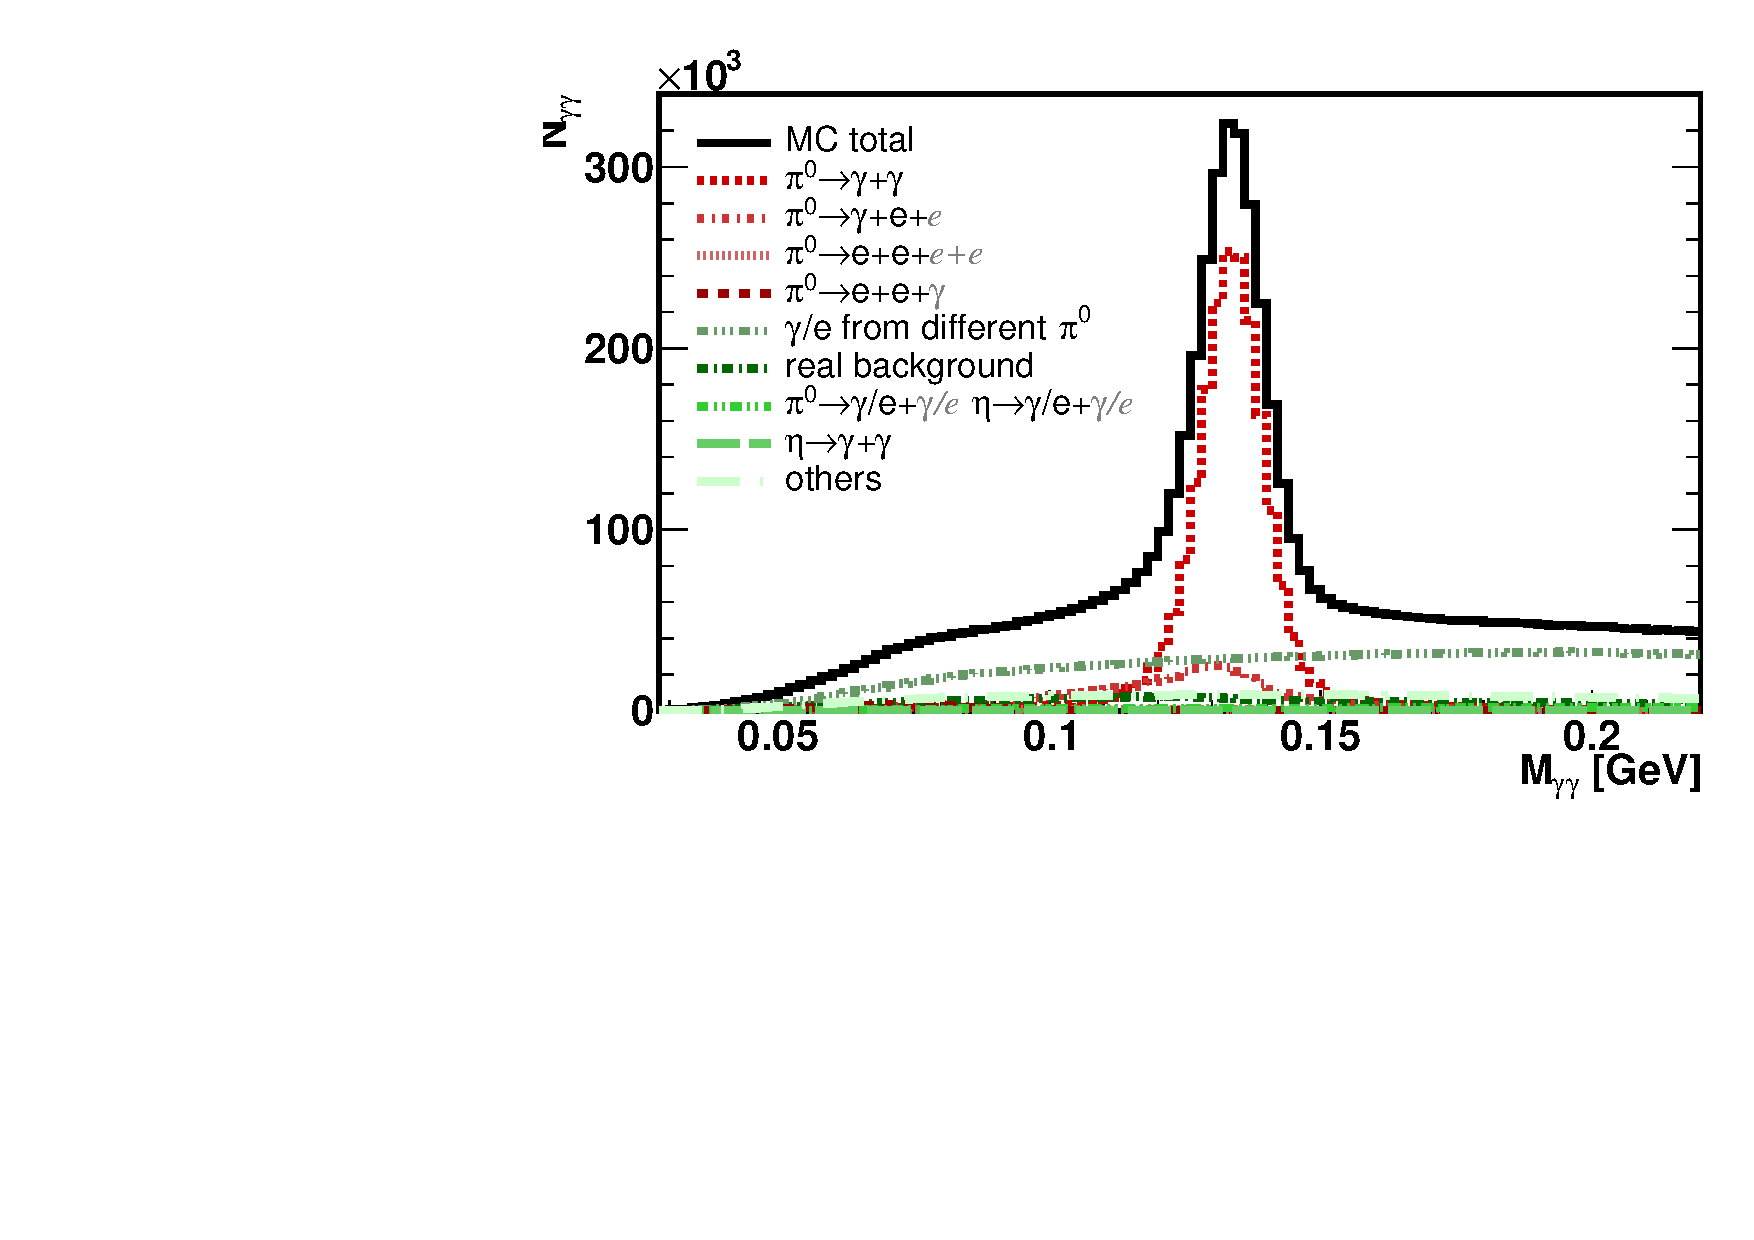
\includegraphics[width=0.60\textwidth,natwidth=600,natheight=400]{figure_dataselection/pi0_component_Z_1.pdf}}
  \subfigure[$\pi^0$ components for $0.4<z<0.5$ ]{\label{fig:mc_singlept_component}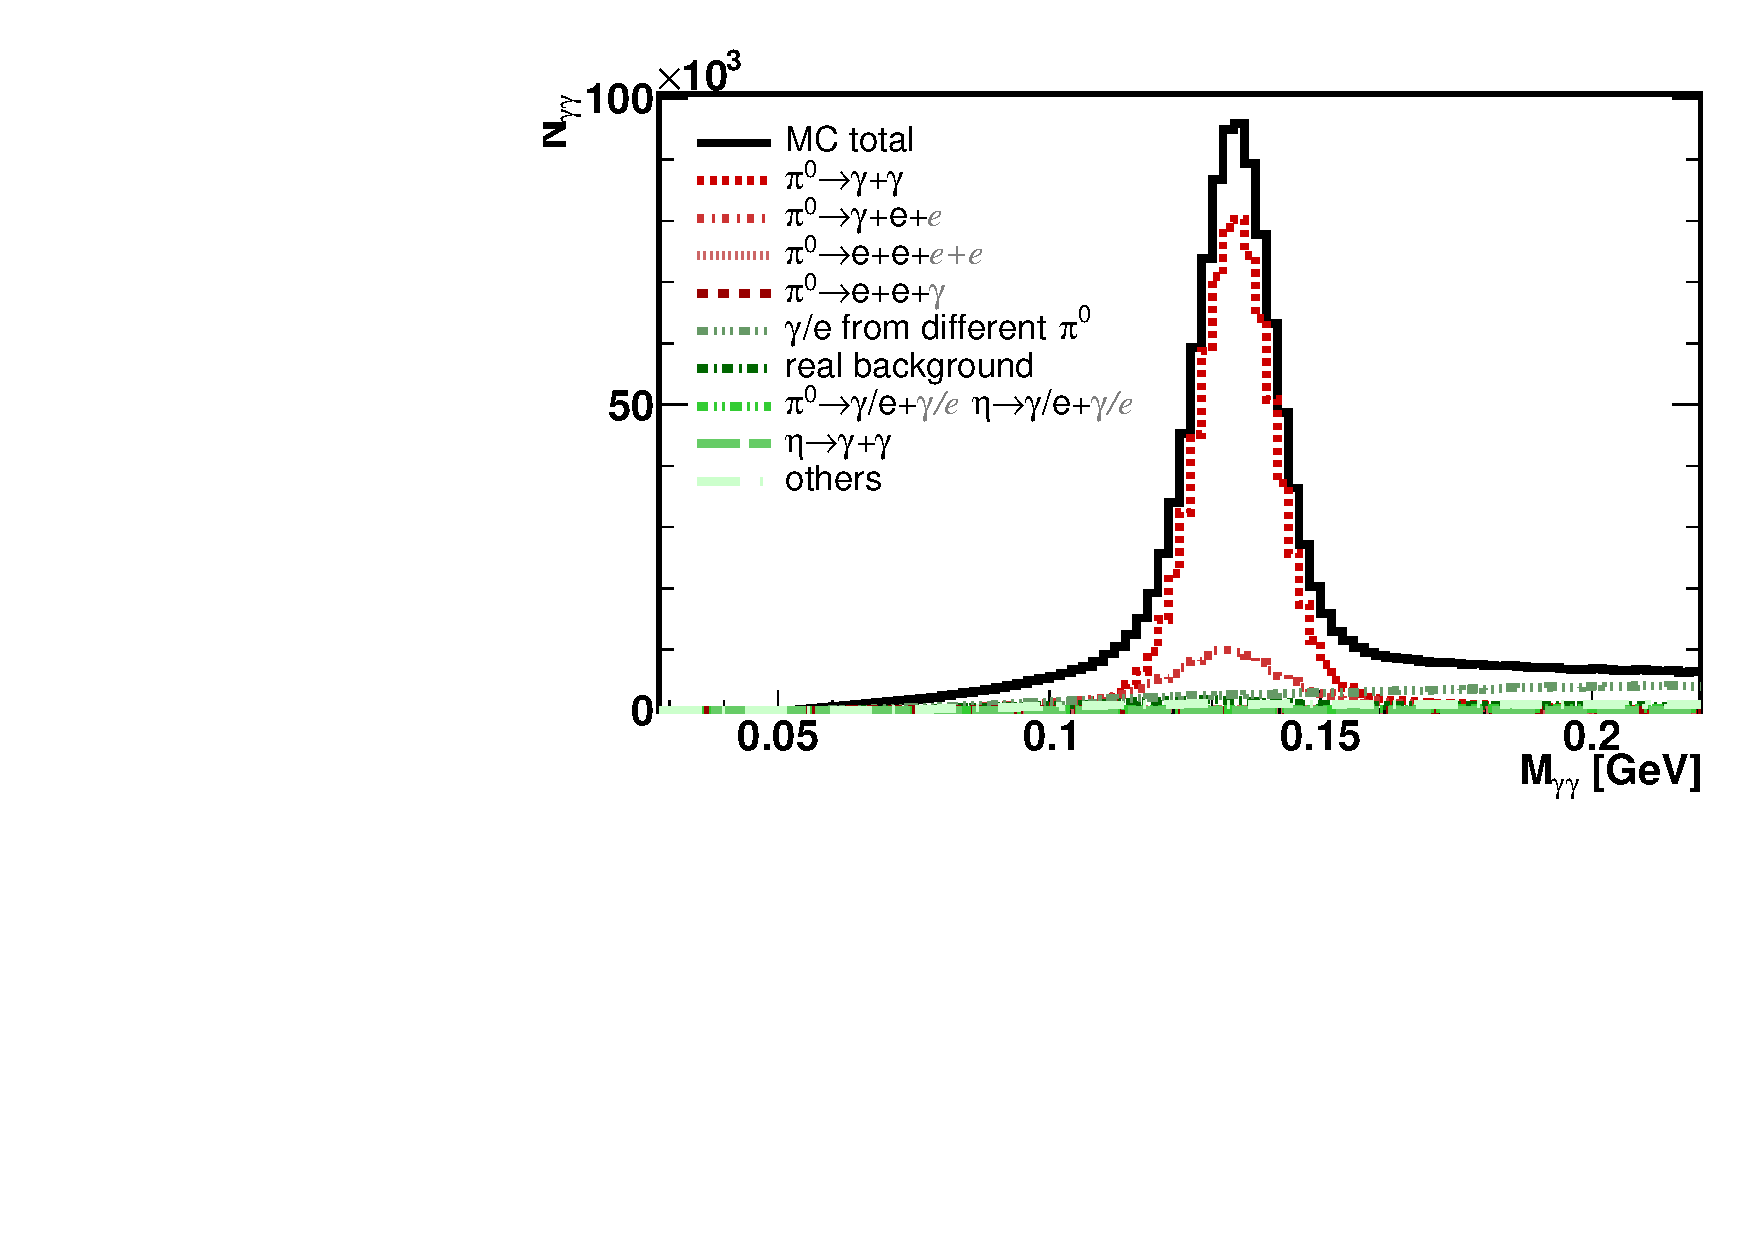
\includegraphics[width=0.60\textwidth,natwidth=600,natheight=400]{figure_dataselection/pi0_component_Z_3.pdf}}
  \caption[Monte Carlo decomposition of the invariant-mass distribution around the \(\pi^{0}\) mass]{All components of $\pi^0$ reconstruction. The red lines are one $\pi^0$ decay to two $\gamma$s and the $\gamma$ may further decay to electrons. Green lines are background. The particles that are not reconstructed are marked in grey in the legend. The invariant mass is then reconstructed from the two remaining decay products. Note that the x-axis label is the reconstructed mass $M_{\gamma\gamma}$ even though the true particle might have been an electron or positron not a $\gamma$.}
  \label{fig:pi0_component}
\end{figure}

As shown in Fig.~\ref{fig:pi0_component} using a MC simulation, the dominant background is combinatorial, e.g., originating from different $\pi^0$. Because both parent mesons carry a Collins asymmetry, it is possible that the asymmetry for this background is also non-zero. Furthermore, a common occurrence is that one of the decay photons decays via $\gamma \rightarrow e^+e^-$ and we identify one of the leptons as a photon. In the MC background method, we define such reconstructed neutral mesons as part of the signal. On the other hand, most of the background contribution comes from photons that do not share a common neutral-meson ancestor. In this simulation, we define all reconstructed $\gamma$ pairs as background when the corresponding true particles cannot be traced back to a common $\pi^0$ parent (or $\eta$ when we want to reconstruct those, but in this channel the backgrounds are small). 


To determine the asymmetry carried on average by the background in real data, we measure the asymmetry in the sidebands and extrapolate into the signal region.
The mass ranges for the sideband asymmetries are $0.065$~GeV$\textup{--}0.085$~GeV, $0.085$~GeV$\textup{--}0.105$~GeV, $0.165$~GeV$\textup{--}0.185$~GeV and $0.185$~GeV$\textup{--}0.205$~GeV. Note that this sideband range is more restrictive then the one that was used for the fit of the invariant-mass region. We choose a region that is closer to the signal window to get a more accurate estimation of the signal under the peak. (The same holds for the case of the $\eta$ discussed below.)

%For the extrapolation of the background asymmetries into the signal region, we assume a linear relation between background asymmetry and invariant mass. 

In Fig.~\ref{fig:bkgasy}  the measured asymmetry is plotted as a function of the invariant mass. A linear fit to the data points, which are plotted at the average mass of the corresponding ranges, is used to determine the background asymmetry in the signal range by evaluating the fit at $x_0$, the average mass of signal range $0.119$~GeV$\textup{--}0.151$~GeV. It can be seen that the linear behavior is consistent with data.

\begin{figure}[t]
  \centering     
  \subfigure[Background $\nicefrac{A^{0\pm}_{12}}{A^L_{12}}$ of $P_{t1}$ bins 0]{\label{fig:bkgasy1}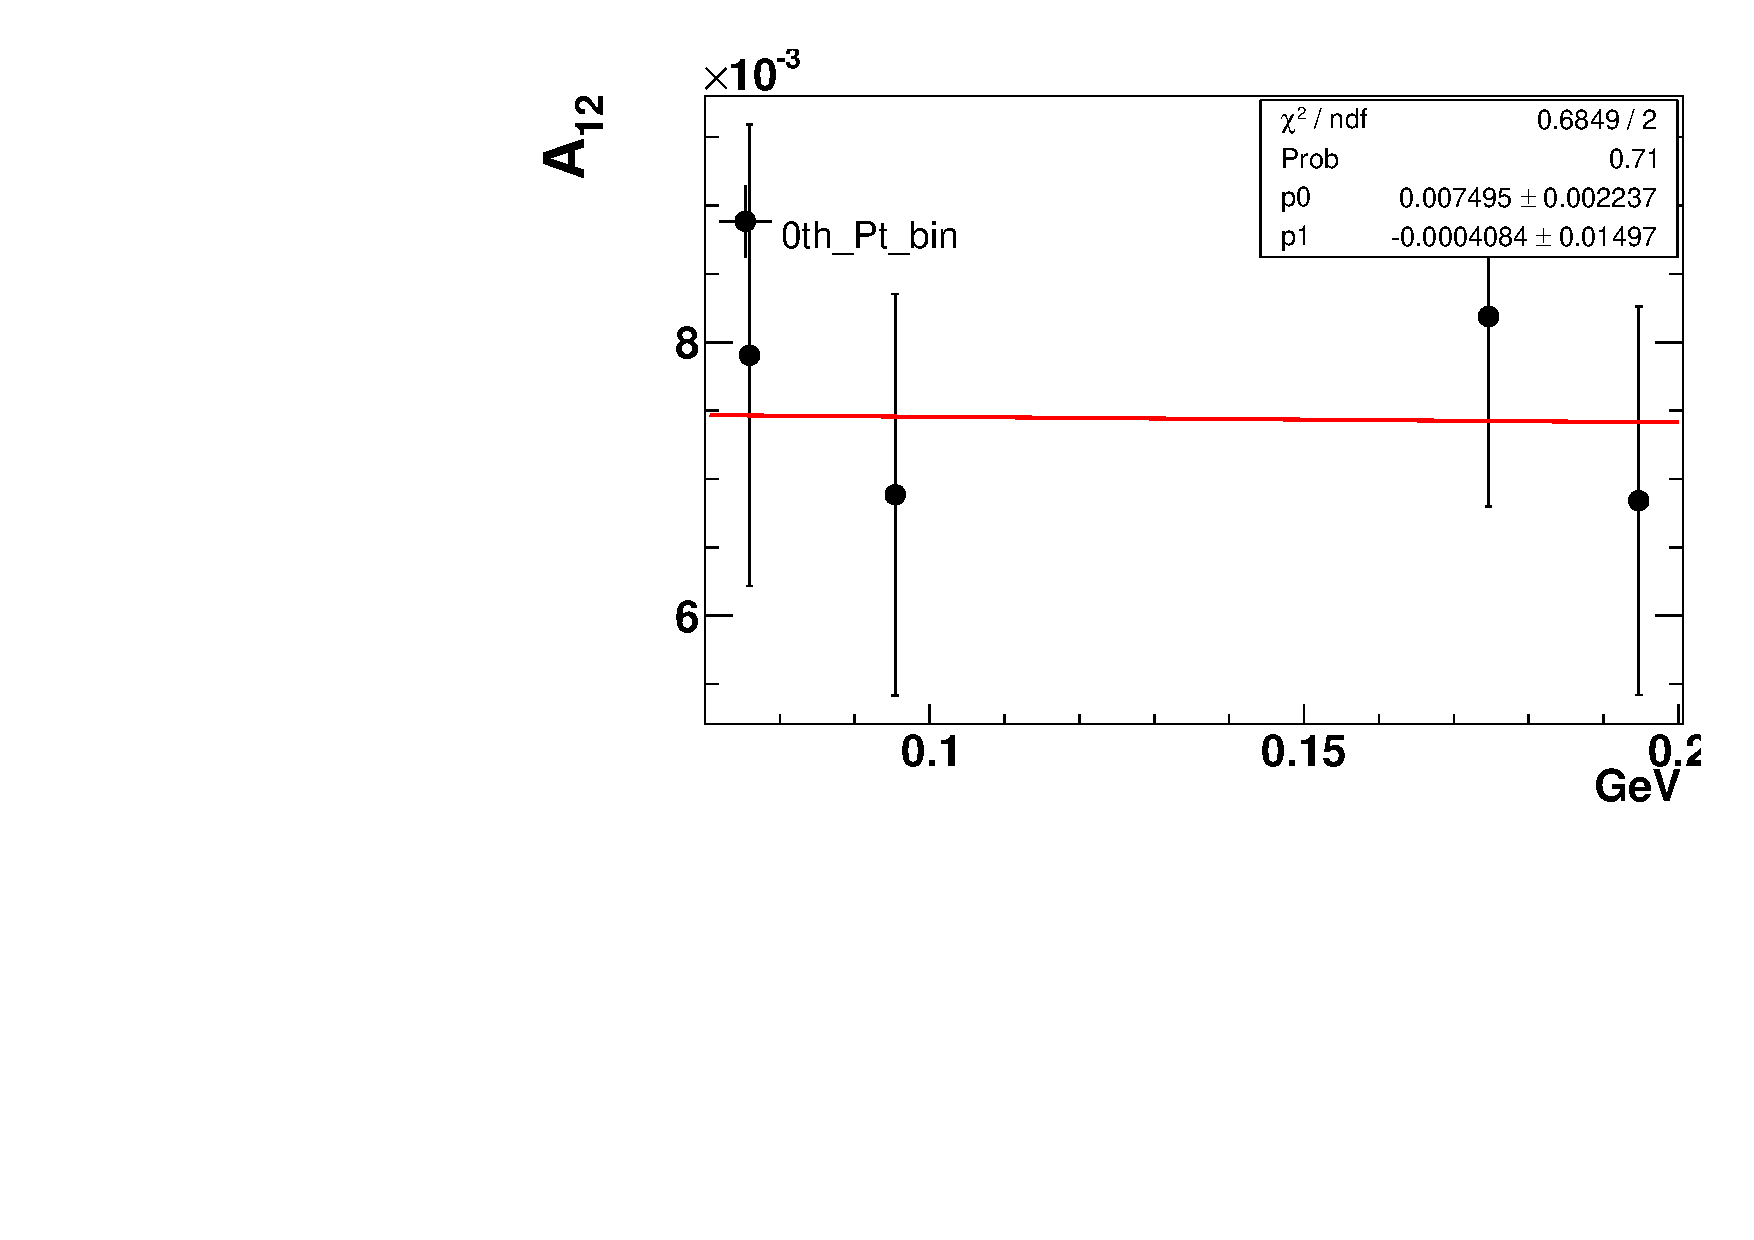
\includegraphics[width=60mm,,natwidth=600,natheight=400]{figure_asy/corrections/SinPt_pi0_Pt_0.pdf}}
  \subfigure[Background $\nicefrac{A^{0\pm}_{12}}{A^L_{12}}$ of $(z_1,z_2)$ bins 5]{\label{fig:bkgasy2}\includegraphics[width=60mm,,natwidth=600,natheight=400]{figure_asy/corrections/ComZ_pi0_Z_5.pdf}}
  \caption{Linear fit to the background asymmetries measured in the invariant-mass sidebands to the $\pi^0$ peak for
     selected kinematic bins.}
  \label{fig:bkgasy}
\end{figure}


Finally, Fig.~\ref{fig:pi0afterbkg} shows the Collins asymmetries before and after background correction.

\begin{figure}[H]
  \centering     
  \subfigure[$z_1$ bins]{\label{fig:pi0afterbkg1}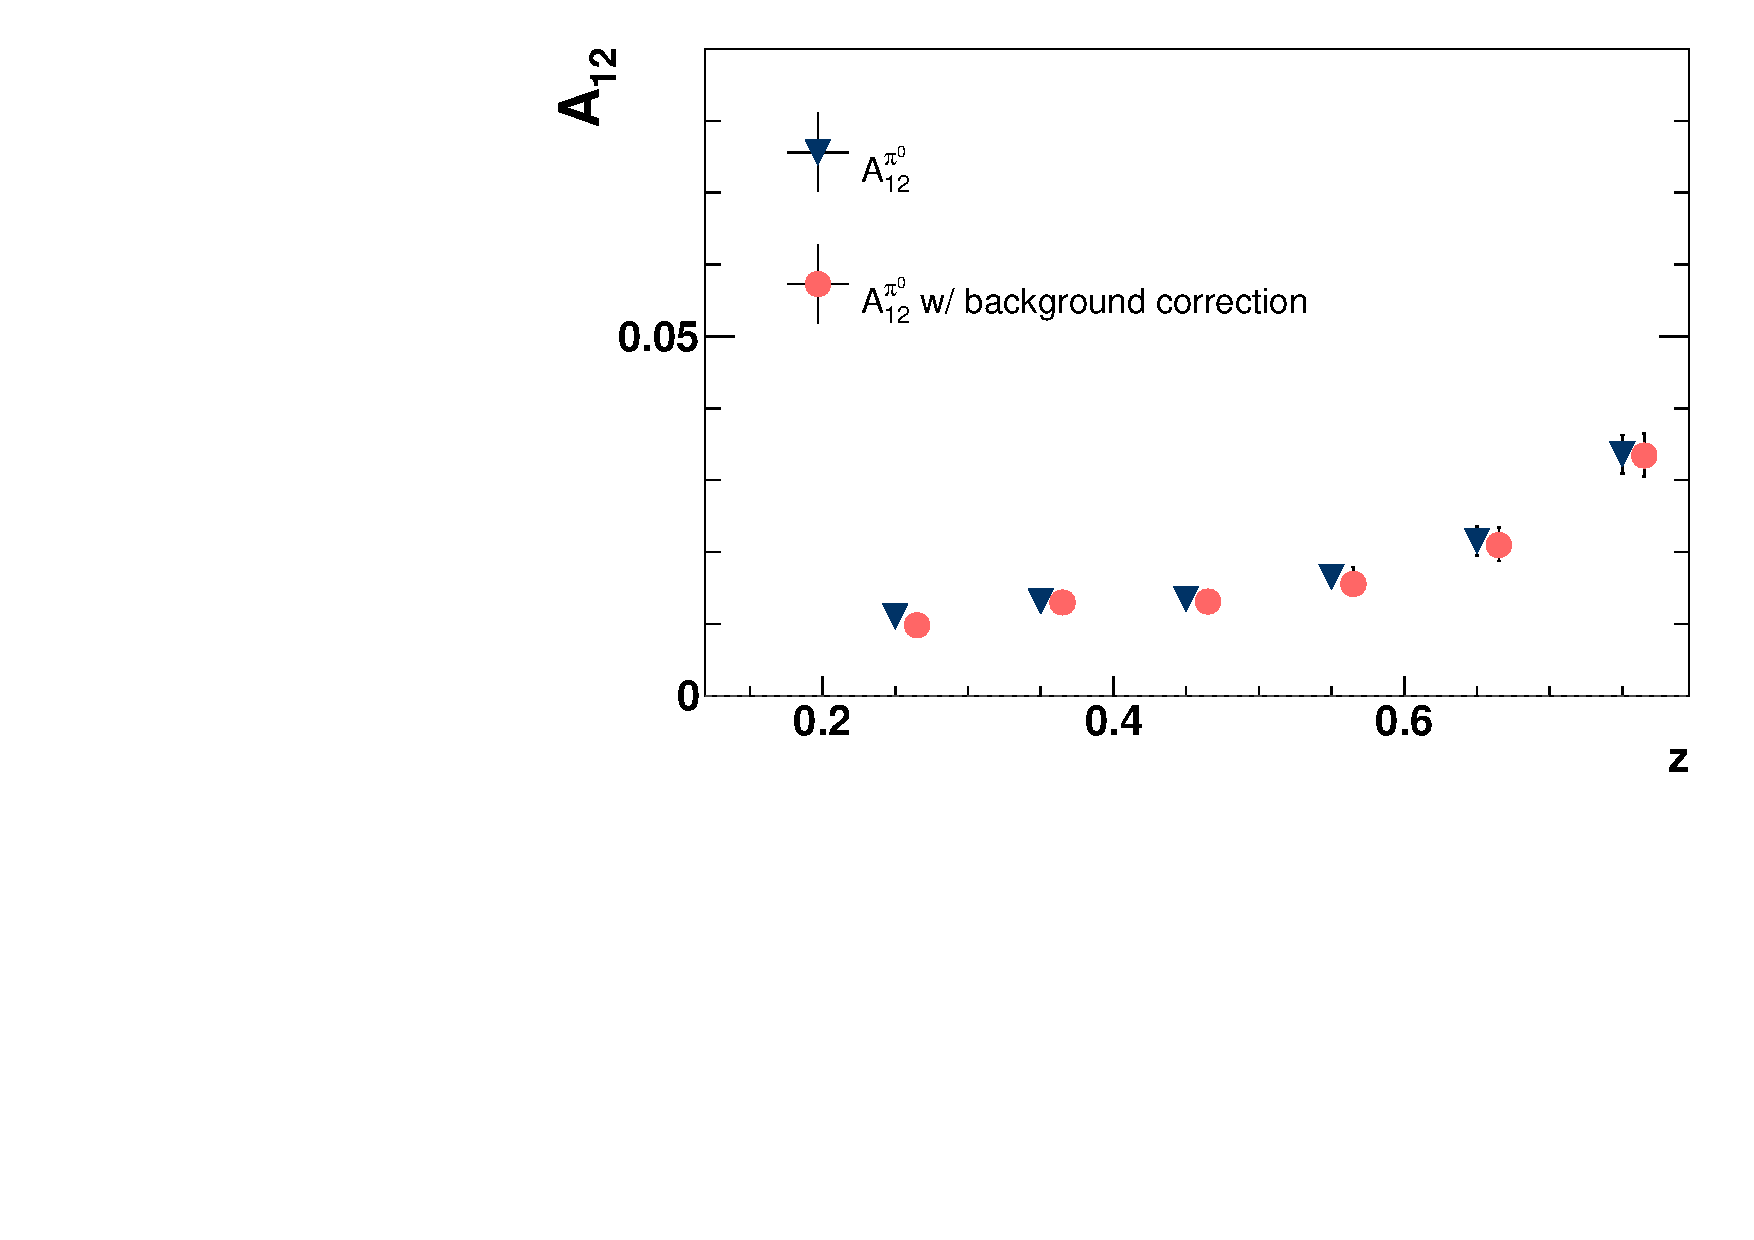
\includegraphics[width=.48\textwidth,natwidth=600,natheight=400]{figure_asy/Pi0BkgCorrection0.pdf}}
  \subfigure[$P_{t1}$ bins]{\label{fig:pi0afterbkg2}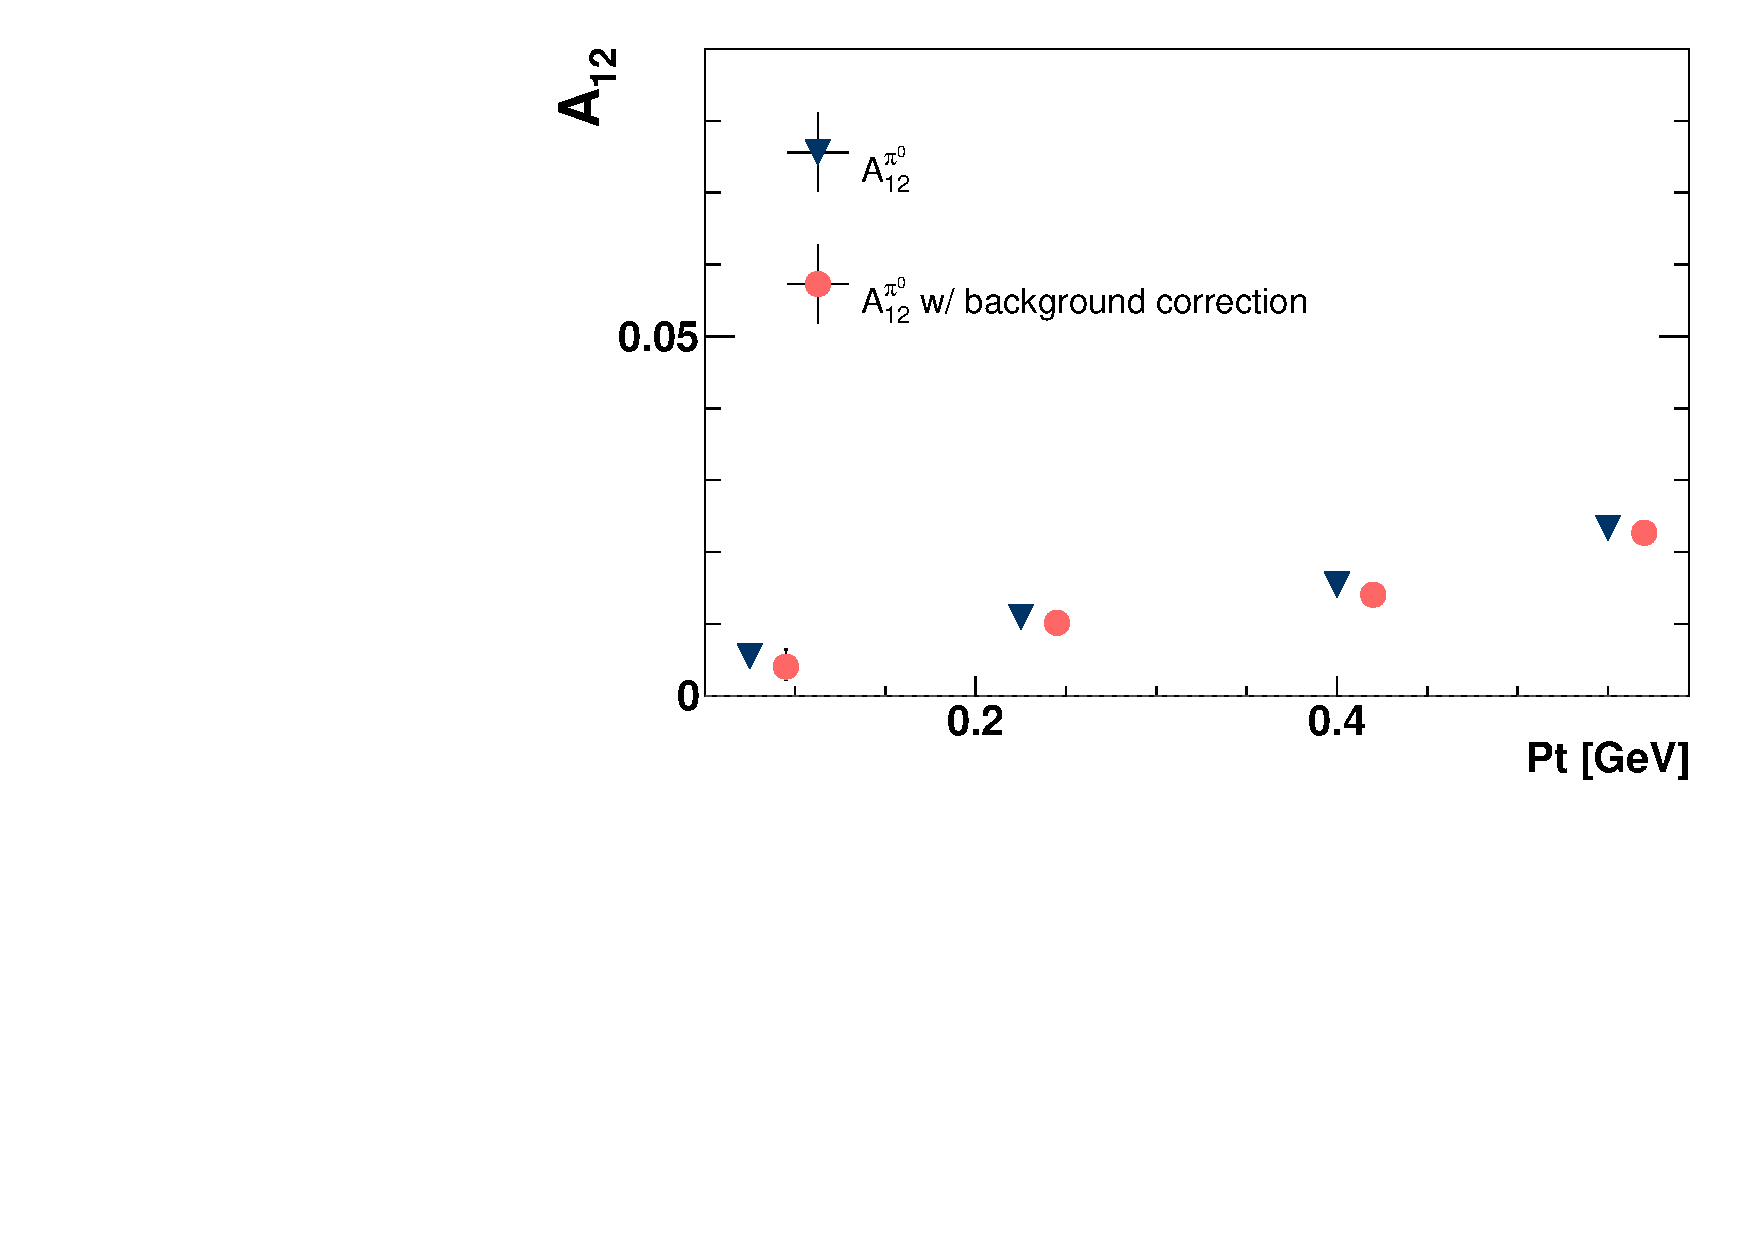
\includegraphics[width=.48\textwidth,natwidth=600,natheight=400]{figure_asy/Pi0BkgCorrection2.pdf}}
  \subfigure[$(z_1,z_2)$ bins]{\label{fig:pi0afterbkg3}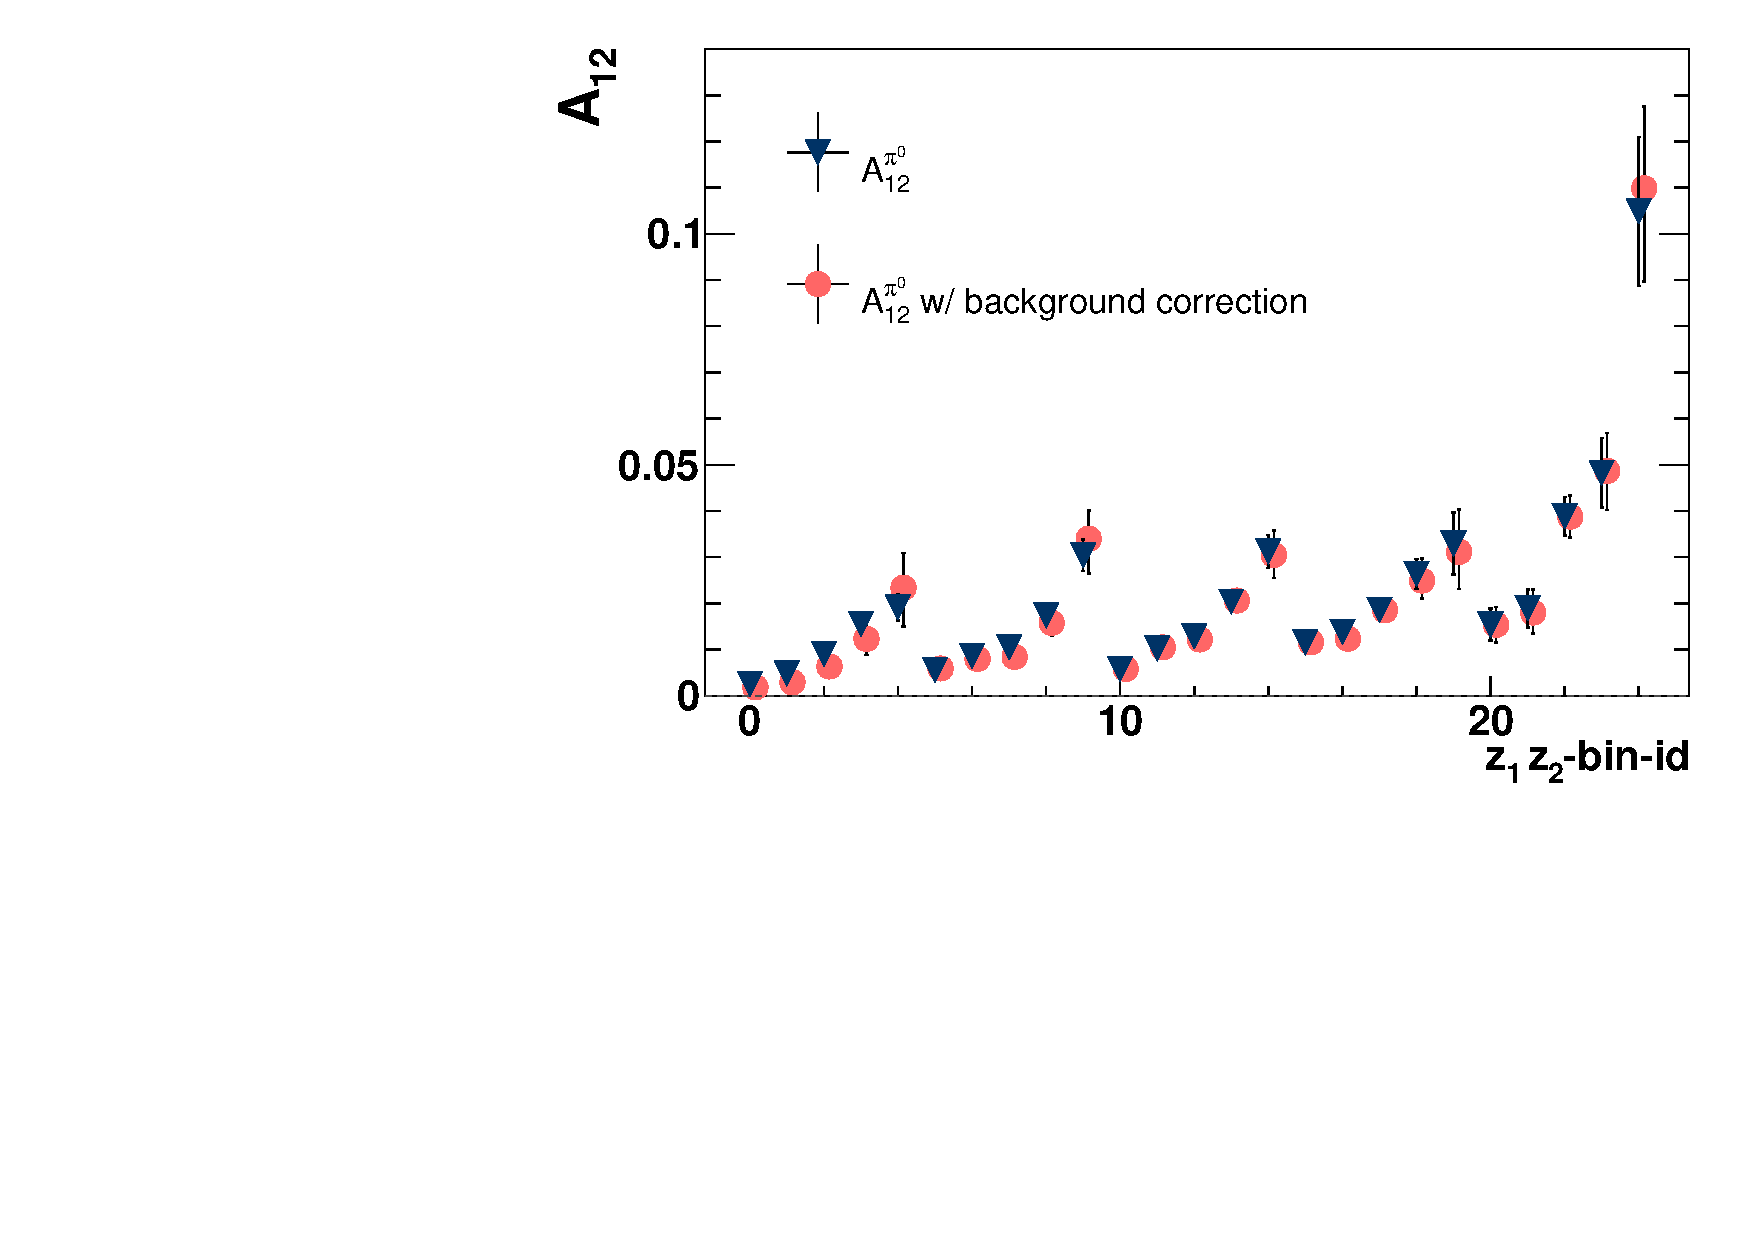
\includegraphics[width=.48\textwidth,natwidth=600,natheight=400]{figure_asy/Pi0BkgCorrection1.pdf}}
  \subfigure[$(P_{t1},P_{t2})$ bins]{\label{fig:pi0afterbkg4}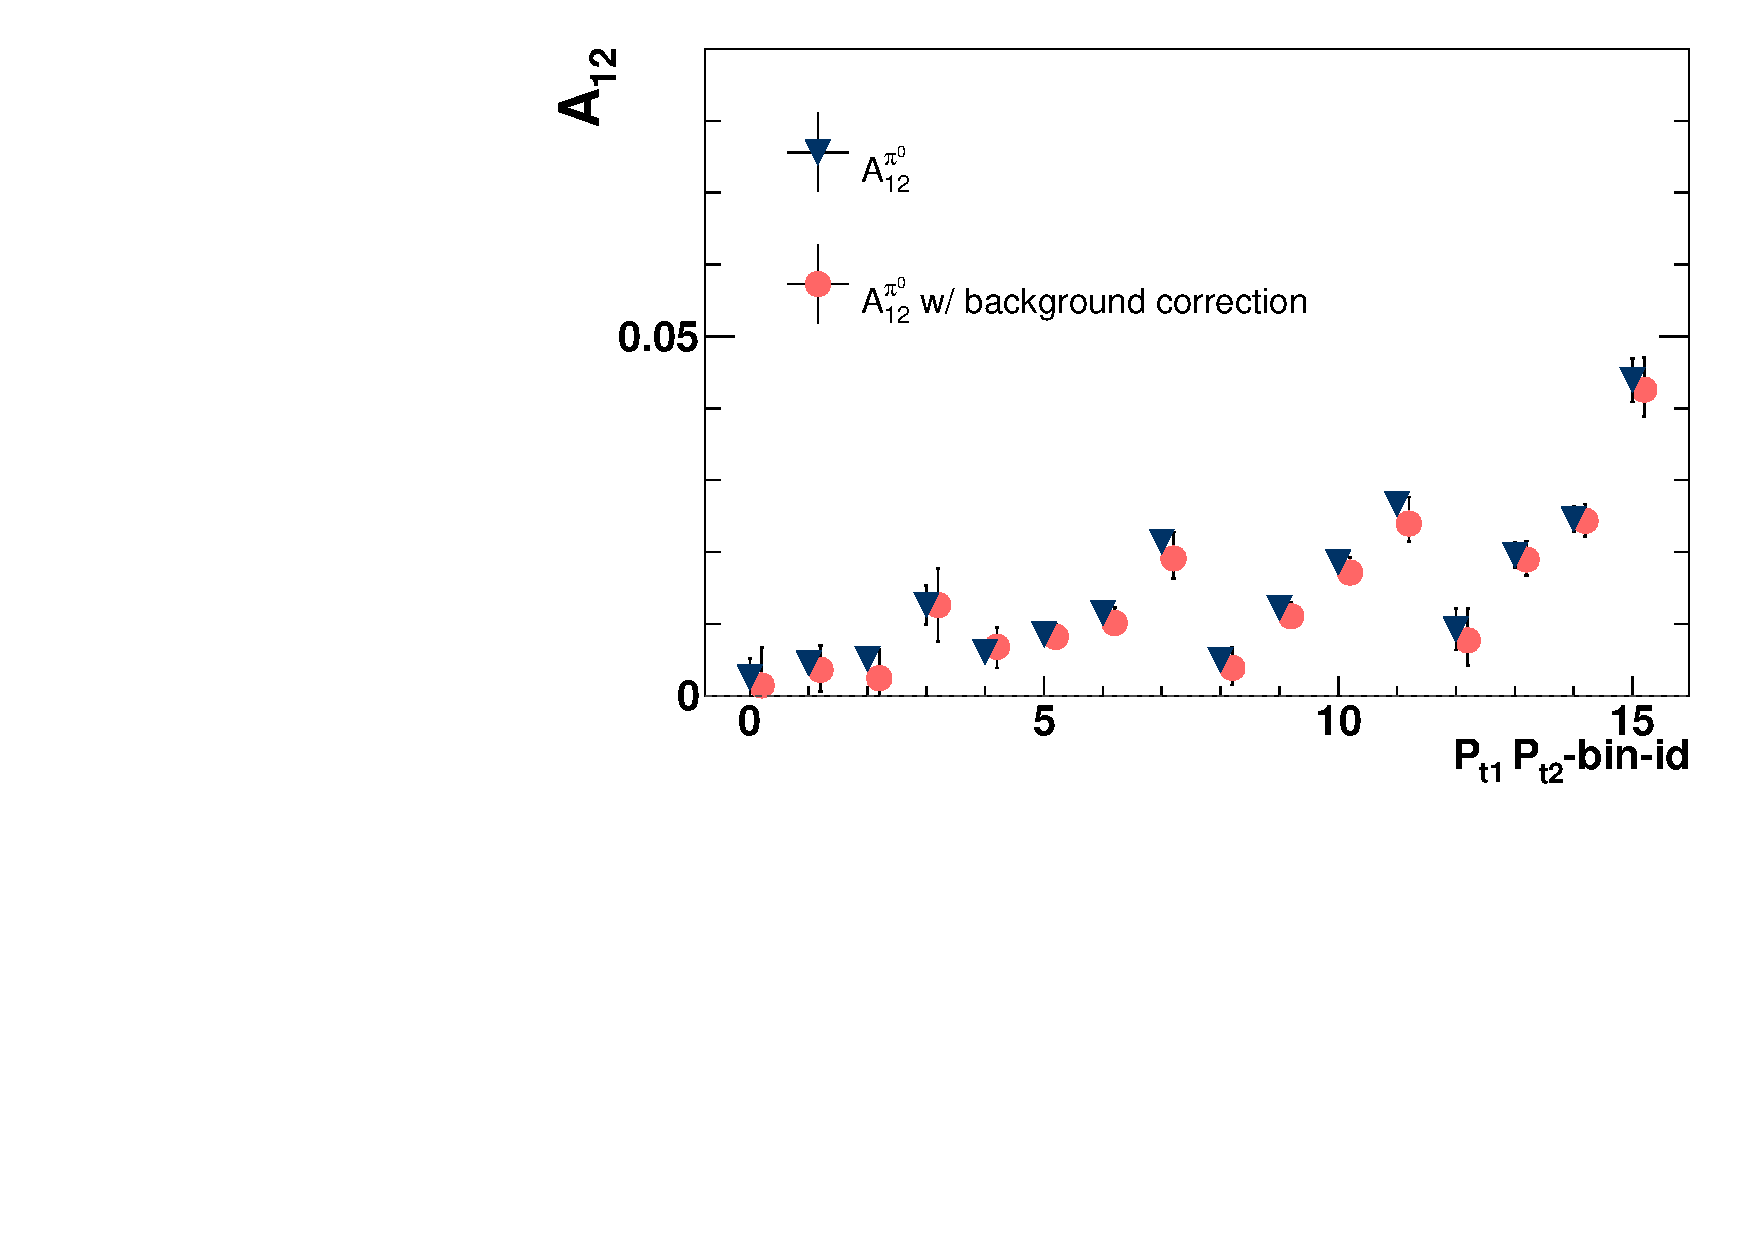
\includegraphics[width=.48\textwidth,natwidth=600,natheight=400]{figure_asy/Pi0BkgCorrection3.pdf}}
\caption[$\pi^0$ double ratio asymmetry $A^{\pi^0}_{12}$ for different kinematic bins]{$\pi^0$ double ratio asymmetry $A^{\pi^0}_{12}$ for different kinematic bins. Blue triangles are raw asymmetries, while pink points are the asymmetries after background correction. \label{fig:pi0afterbkg}}
\end{figure}

\subsubsection{\texorpdfstring{$\eta$ Background Correction}{eta background correction}}
\begin{figure}[H]
  \centering     
  \subfigure[$0.5<z<0.6$ ]{\label{fig:etacomponent1}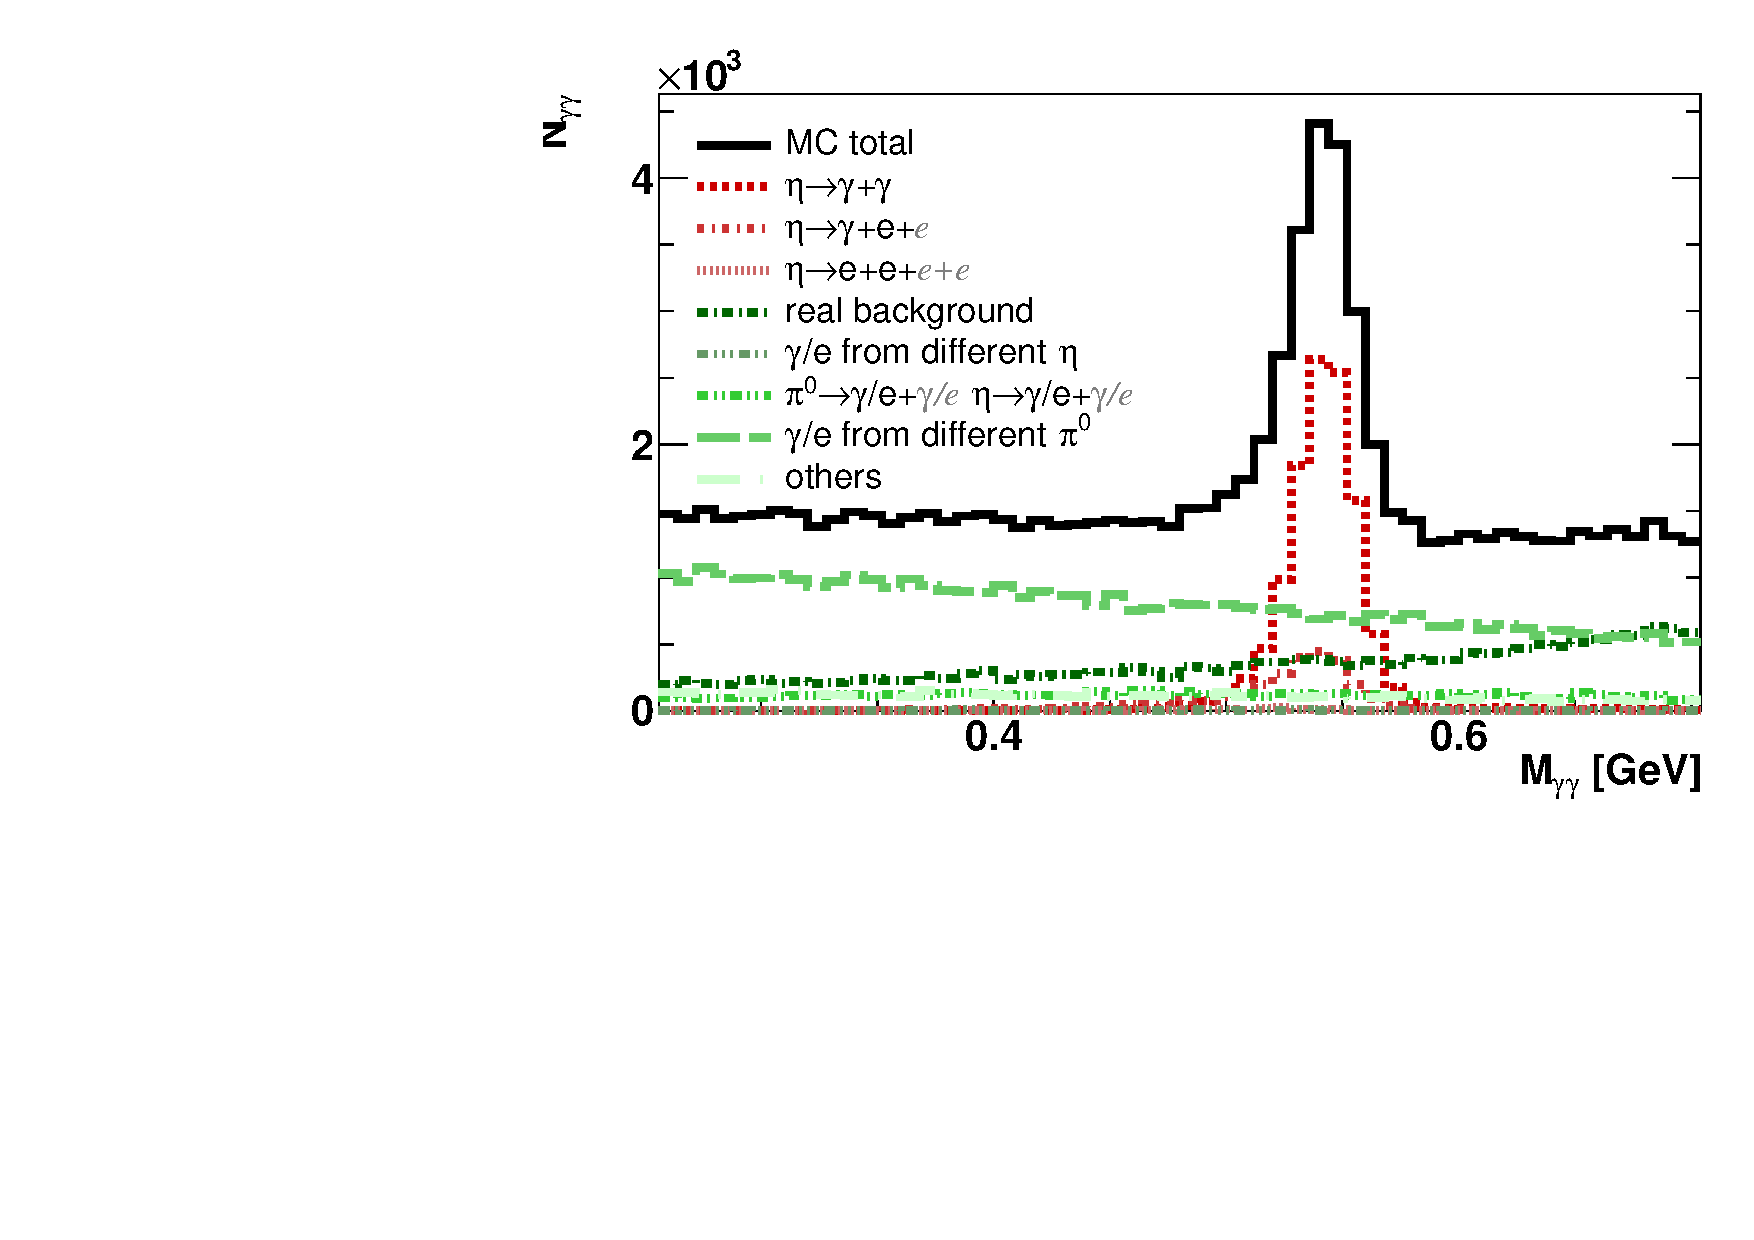
\includegraphics[width=.48\textwidth,natwidth=250,natheight=100]{figure_dataselection/eta_component_Z_5.pdf}}
  \subfigure[0.3~GeV $<P_t<$ 0.5~GeV]{\label{fig:etacomponent2}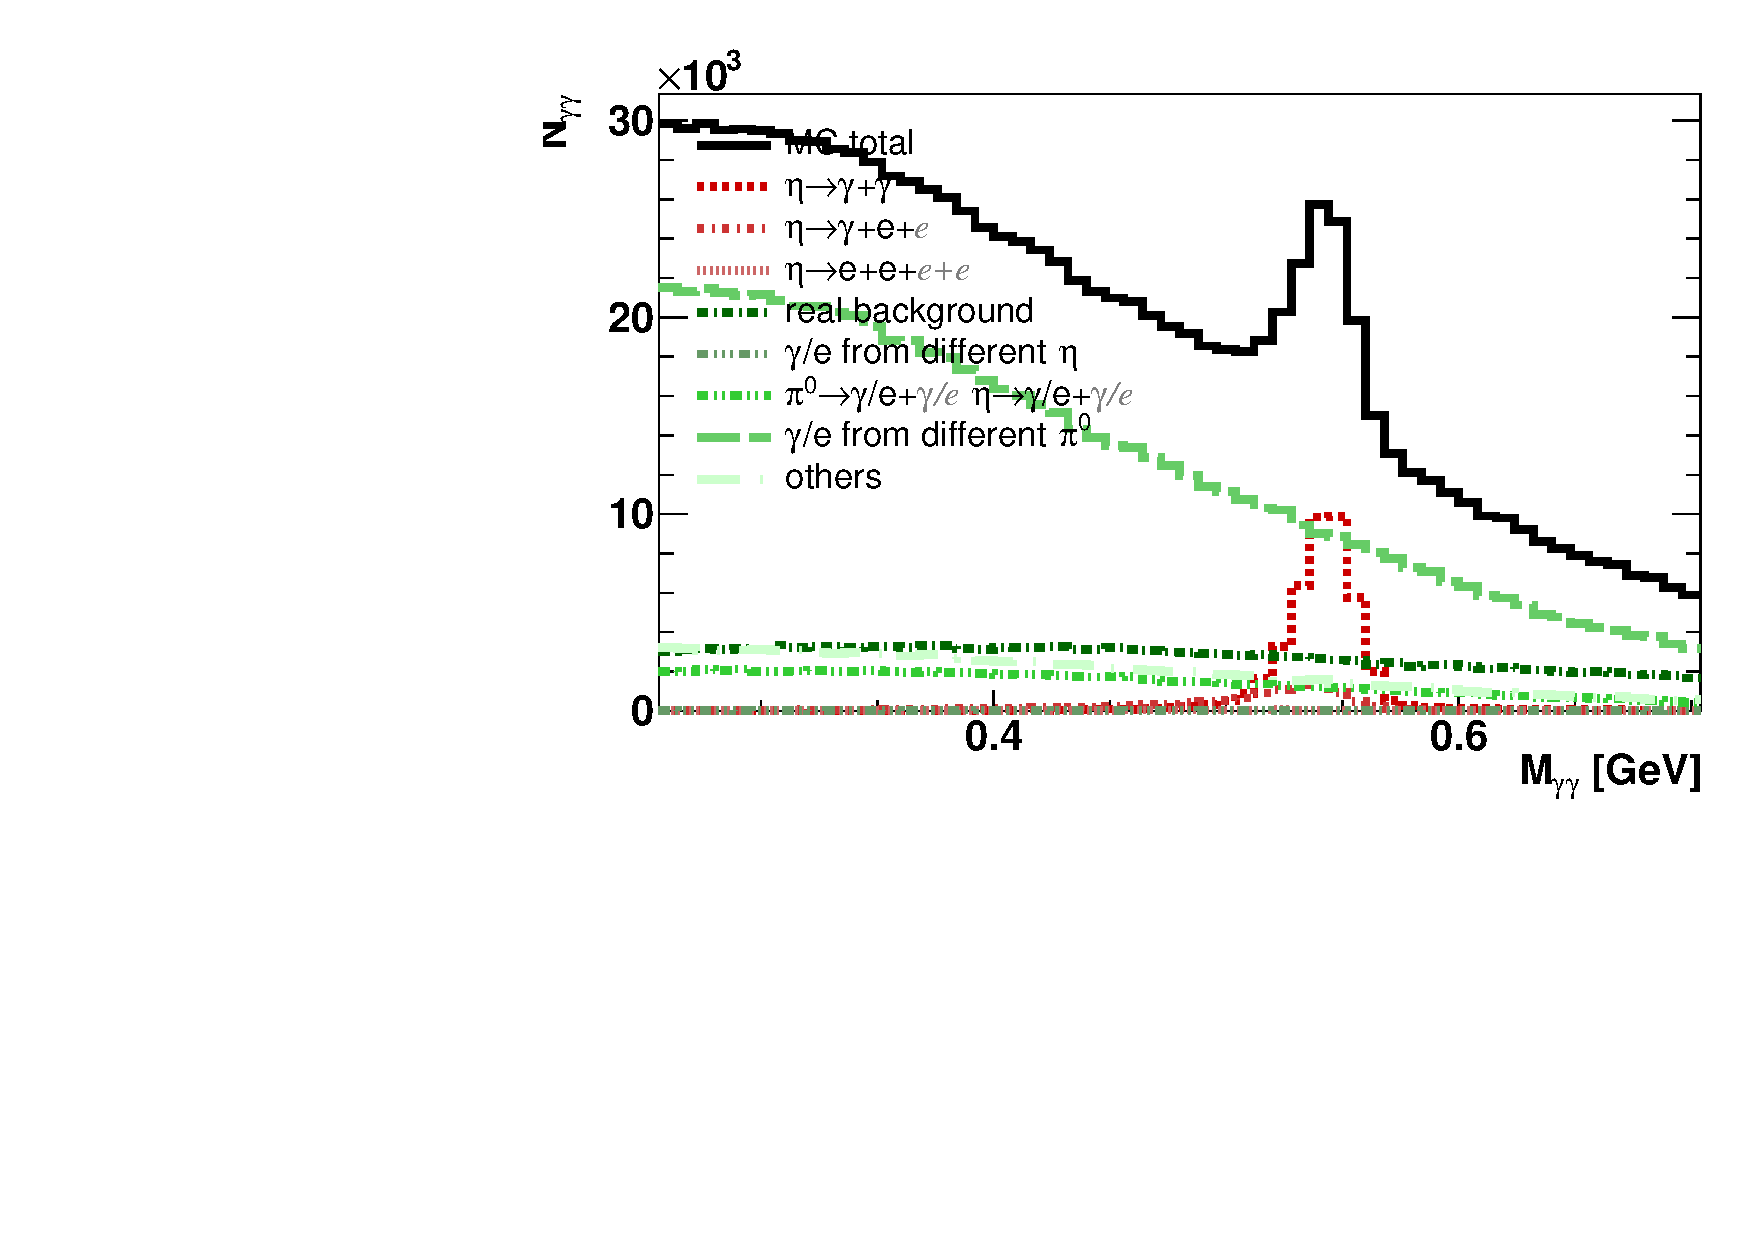
\includegraphics[width=.48\textwidth,natwidth=250,natheight=100]{figure_dataselection/eta_component_Pt_2.pdf}}
  \caption[Monte Carlo decomposition of the invariant-mass distribution around the \(\eta\) mass]{Monte Carlo decomposition of the $\eta$ invariant mass distributions. The missing particles during reconstruction are marked in grey in the legend.}
  \label{fig:etacomponent}
\end{figure}
Similar to the $\pi^0$ case, components of the $\eta$ invariant-mass distribution were studied in a simulation. In Fig.~\ref{fig:etacomponent} it can be seen that $\gamma$'s and electrons originally coming from $\pi^0$ contribute the most to the background. The background asymmetry can be estimated in the same way as done for the $\pi^0$ background. The sidebands  selected are 0.4638--0.4878~GeV, 0.4398--0.4638~GeV, 0.5838--0.6078~GeV and 0.6078--0.6318~GeV. We construct the function $A_{bkg}(m)$ using a linear fit from which we estimate  $A_{bkg}(m_{\eta})$. The uncertainty of the background asymmetry is calculated through Eq.~\eqref{eqn:asybkgerr}.

As described in Section~\ref{sec:etafitsection}, the $\eta$ invariant mass can be fitted using two methods. One method is to fit the background with a polynomial function to the sidebands and then subtract the linearly extrapolated background from the total in the signal region. The other one is to fit the sideband and signal region using a polynomial function plus the Crystal Ball function. The purity is obtained through the Crystal Ball fitting method.%To get the uncertainty of purity measurement, pol(6), pol(5) and pol(4) are used as fitting functions for first method. Crystal Ball function and pol(3) are used together as second method. 

Again, we use Eq.~\eqref{eqn:bkgcorr} to calculate the signal asymmetry $A_{sig}$. Figure~\ref{fig:etaafterbkg} shows the result of the $\eta$ Collins double-ratio asymmetry after background correction. 

\begin{figure}[H]
  \centering     
  \subfigure[$z_1$ bins]{\label{fig:etaafterbkg1}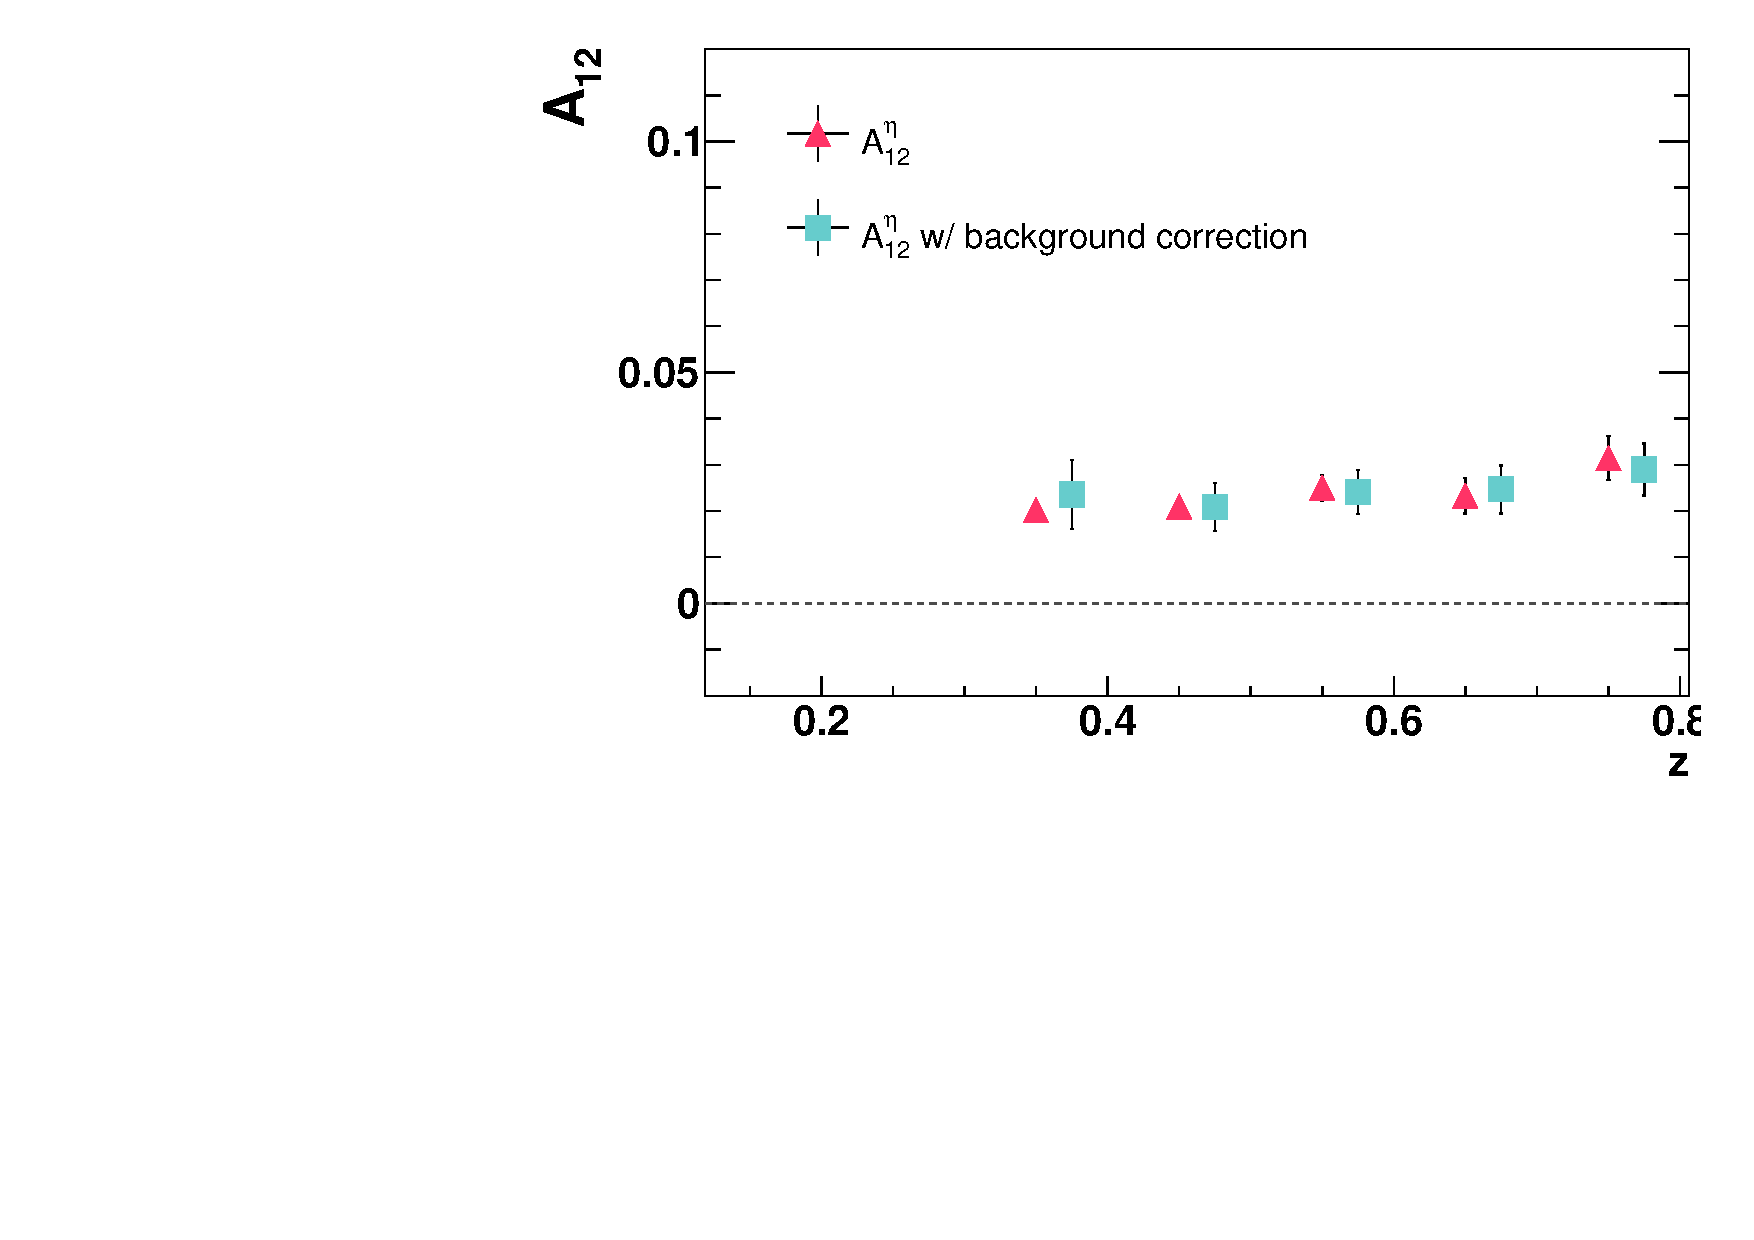
\includegraphics[width=.48\textwidth,natwidth=600,natheight=400]{figure_asy/EtaBkgCorrection0.pdf}}
  \subfigure[$P_{t1}$ bins]{\label{fig:etaafterbkg3}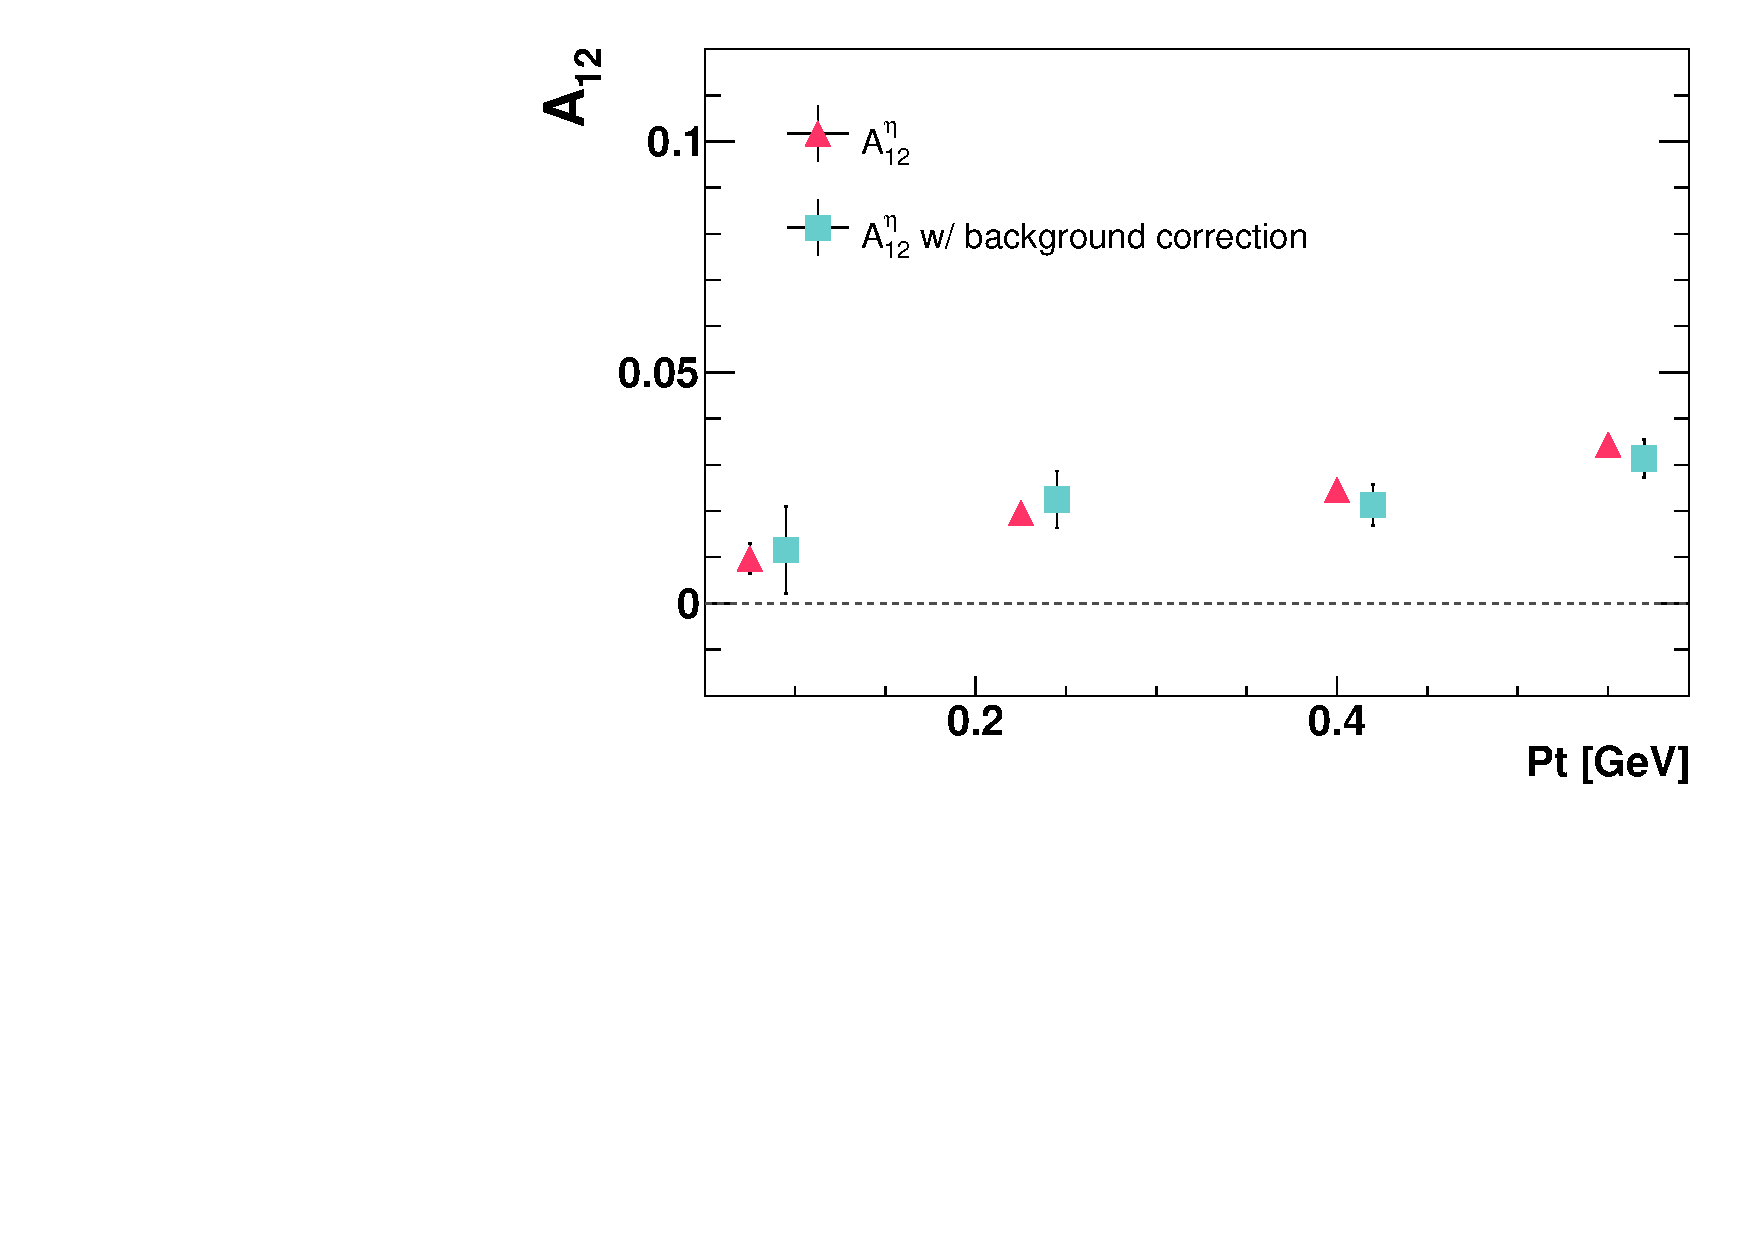
\includegraphics[width=.48\textwidth,natwidth=600,natheight=400]{figure_asy/EtaBkgCorrection2.pdf}}
  \subfigure[$(z_1,z_2)$ bins]{\label{fig:etaafterbkg2}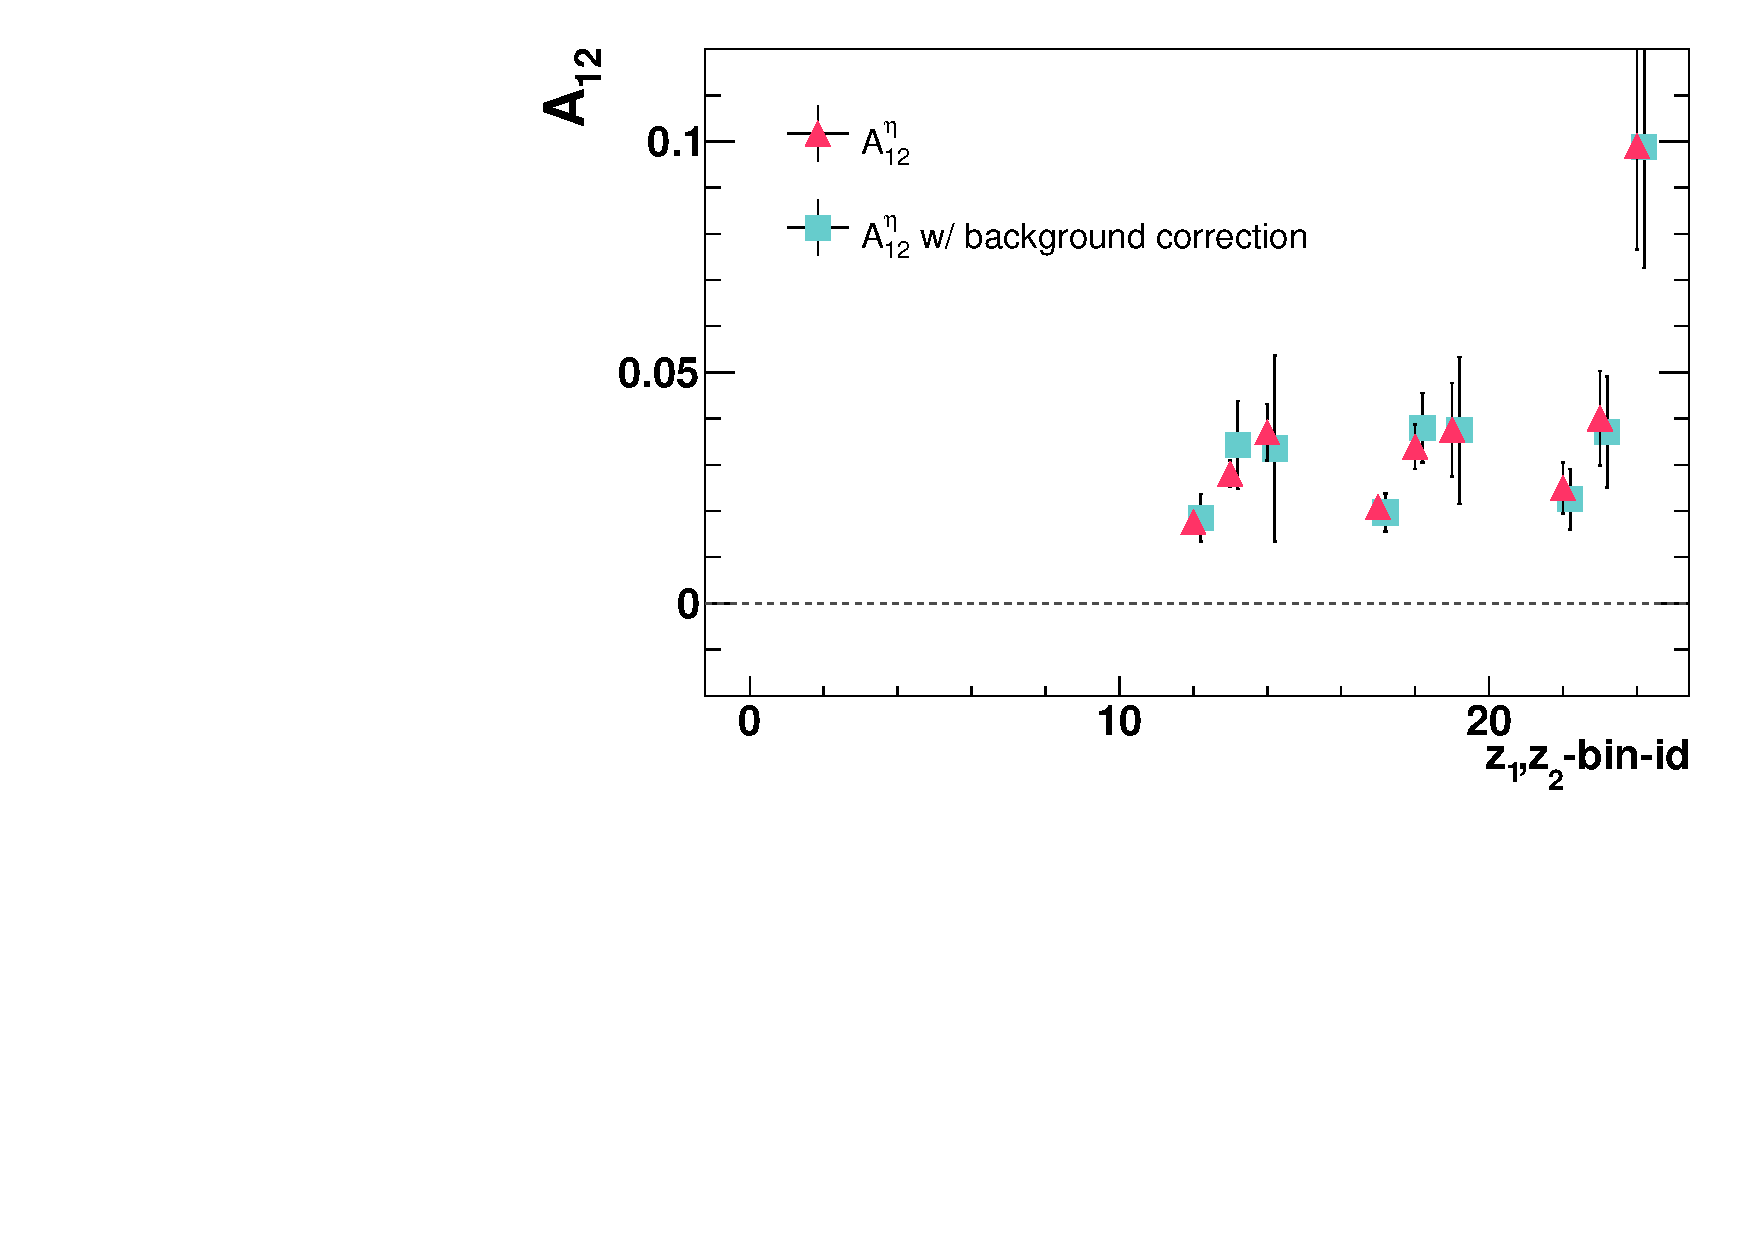
\includegraphics[width=.48\textwidth,natwidth=600,natheight=400]{figure_asy/EtaBkgCorrection1.pdf}}
  \subfigure[$(P_{t1},P_{t2})$ bins]{\label{fig:etaafterbkg4}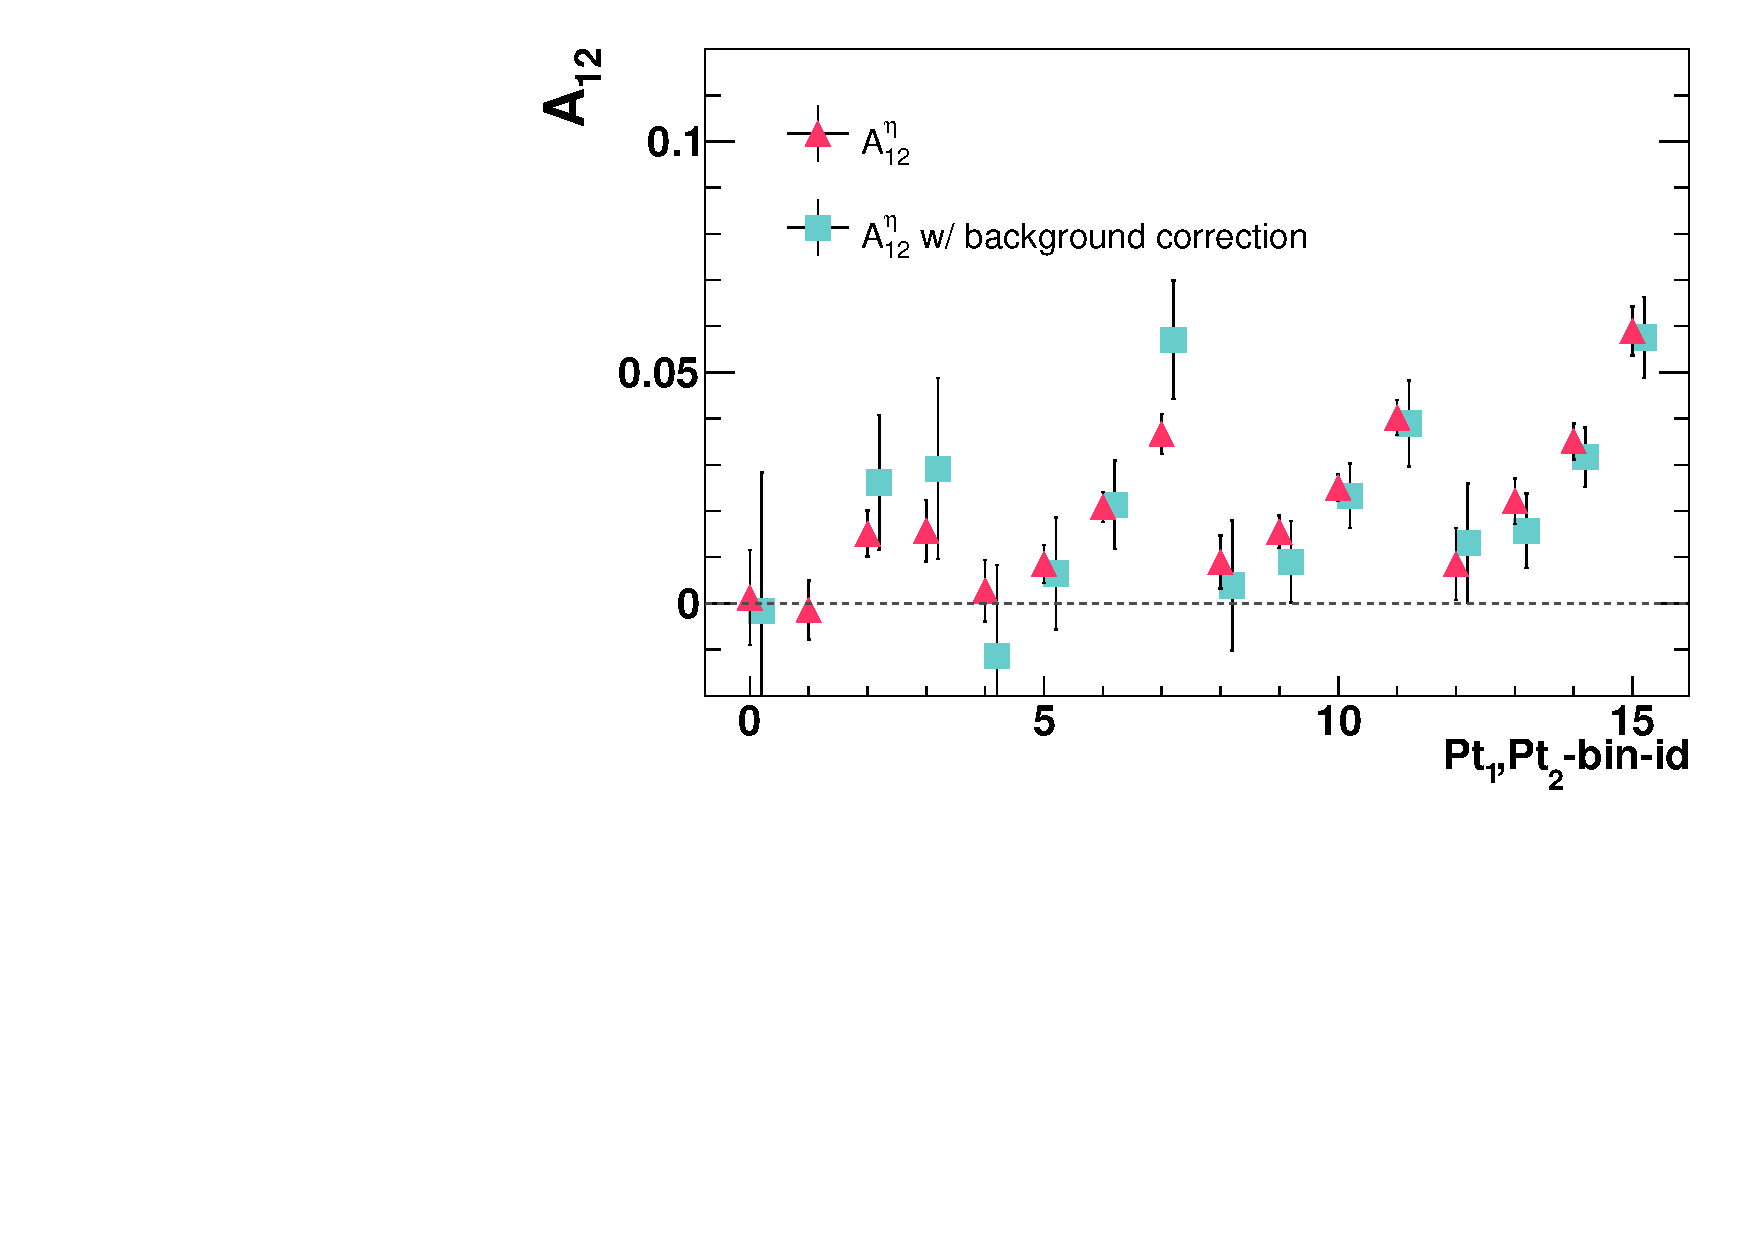
\includegraphics[width=.48\textwidth,natwidth=600,natheight=400]{figure_asy/EtaBkgCorrection3.pdf}}
  \caption[$\eta$ double ratio asymmetry $A^{\eta}_{12}$ for different kinematic bins]{$\eta$ double ratio asymmetry $A^{\eta}_{12}$ for different kinematic bins. The pink triangles are the originally measured raw asymmetries. Blue squares are asymmetries after background correction.}
  \label{fig:etaafterbkg}
\end{figure}

%%%%---> got till here so far



\subsection{\texorpdfstring{Thrust-Smearing Correction}{Thrust smearing correction}}
\label{sec:smearingcorrection}

As discussed earlier, we use the thrust axis of the event as a proxy for the $q\bar{q}$ axis since the later is not an observable and  also cannot be identified in the simulation that we are using beyond leading order.
However, the reconstructed thrust axis will exhibit some deviation from the true thrust axis due to the momentum smearing and effects due to unobserved particles. We identify the true thrust axis as the thrust axis that is obtained from Eq.~\ref{eq:thrust} using all particles in the event that are stable. In the following we will call this the  {\em stable-thrust} (axis). As a technical note, in the simulation, stable particles are identified by requiring isthep=1.

\begin{figure}[h]
\tiny
  \centering     
 \subfigure[Collins angles based on {\em stable-thrust}.]{\label{fig:beforeillustr}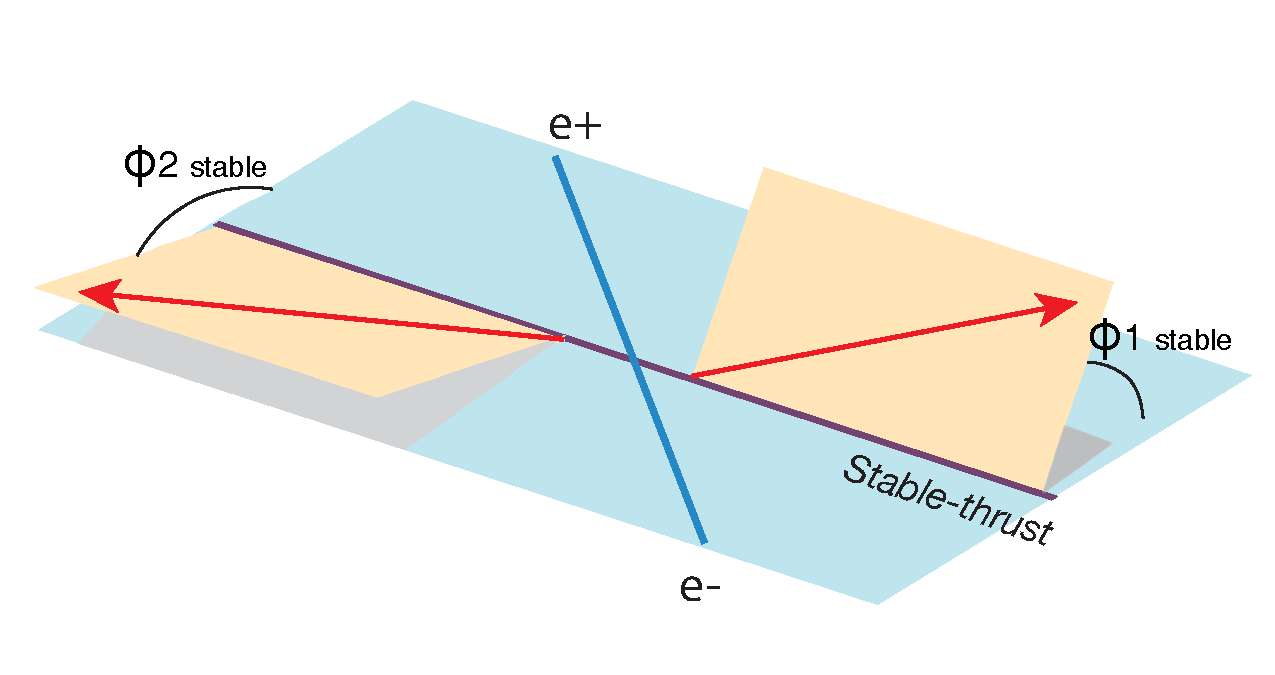
\includegraphics[width=.49\textwidth,natwidth=600,natheight=400]{figure_theory/BeforeSmear.pdf}}
 \subfigure[Collins angles based on {\em measured-thrust}]{\label{fig:afterillustr}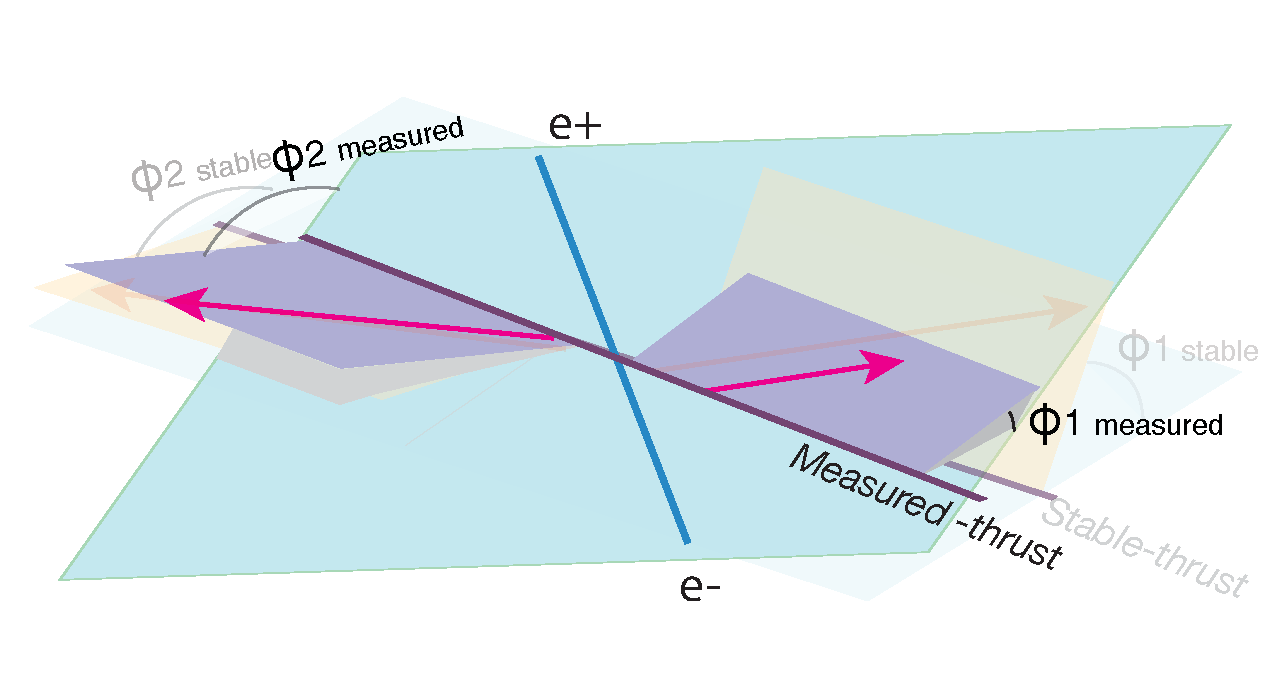
\includegraphics[width=.49\textwidth,natwidth=600,natheight=400]{figure_theory/AfterSmear.pdf}}
  \caption[Illustration of the Collins angle before and after smearing]{Illustration of the Collins angle before and after smearing. The {\em measured-thrust} does not align with the {\em stable-thrust} and the plane spanned by thrust and electrons is changed. During this smearing process, Collins angles are altered which leads to the dilution of Collins effect.}
  \label{fig:SmearIllustr}
\end{figure}

 Figure~\ref{fig:SmearIllustr} illustrates the difference between the measured thrust and the stable thrust as well as the resulting smearing effect. Obviously the smearing effect for each identified hadron depends on its respective kinematics. But in general, the smearing will dilute the Collins effect. In addition to the smearing of the Collins angle, there are also bin-migration effects to consider. While $z$-bin migration is minimal, since our bin width is relatively large and $z$ is measured with respect to the $\sqrt{s}$ scale, the $P_t$ is measured with respect to the not precisely known thrust axis and is thus more susceptible to smearing.


\subsubsection{\texorpdfstring{Re-weighting Method}{Re-weighting Method}} 
\label{sec:pi0thrustcorrection}
A common method to evaluate smearing effects is to use re-weighting. Here we weight events in simulation according to their true kinematics and then estimate the effect of the smearing by comparing the reconstructed values with the input values.
 %A cosine modulation about the thrust axis might get distorted (and usually reduced in amplitude) through the finite resolution of the thrust-axis reconstruction. 
 Here we re-weight our Monte Carlo simulation based on the distribution of hadron pairs about the {\em stable-thrust} axis. Based on an injected asymmetry $A_i$ we assign an event weight of $1+A_i*\cos\phi_{12}^{\text{stable}}$, where $\phi_{12}^\text{stable}$ is the Collins angle about the stable-thrust axis.

Collins asymmetries are then measured from an event-by-event weighted set using the measured Collins angle of all $\pi^0$ candidates in the signal window. 
Ideally, if the thrust axis duplicates the stable thrust exactly, the injected and the measured asymmetries should be equal. 
However, if the thrust axis diverges from the stable-thrust axis, the Collins asymmetry will be diluted thus leading to a lower measured asymmetry. 
The dilution ratio can be estimated to correct the measured asymmetry. Each kinematic bin will be corrected according to  the dilution estimated for that kinematic bin.

To properly account for the bin migration mentioned before, the injected asymmetry has to be chosen such that the resulting asymmetry is similar to the measured asymmetry after smearing. 
As explained above, this is mainly important for the $P_t$ dependence. 
Figure~\ref{fig:weightpi0} shows an example of re-weighted asymmetries after smearing.

\begin{figure}[H]
  \centering     
  \subfigure[$z_1$ bins]{\label{fig:weightpi01}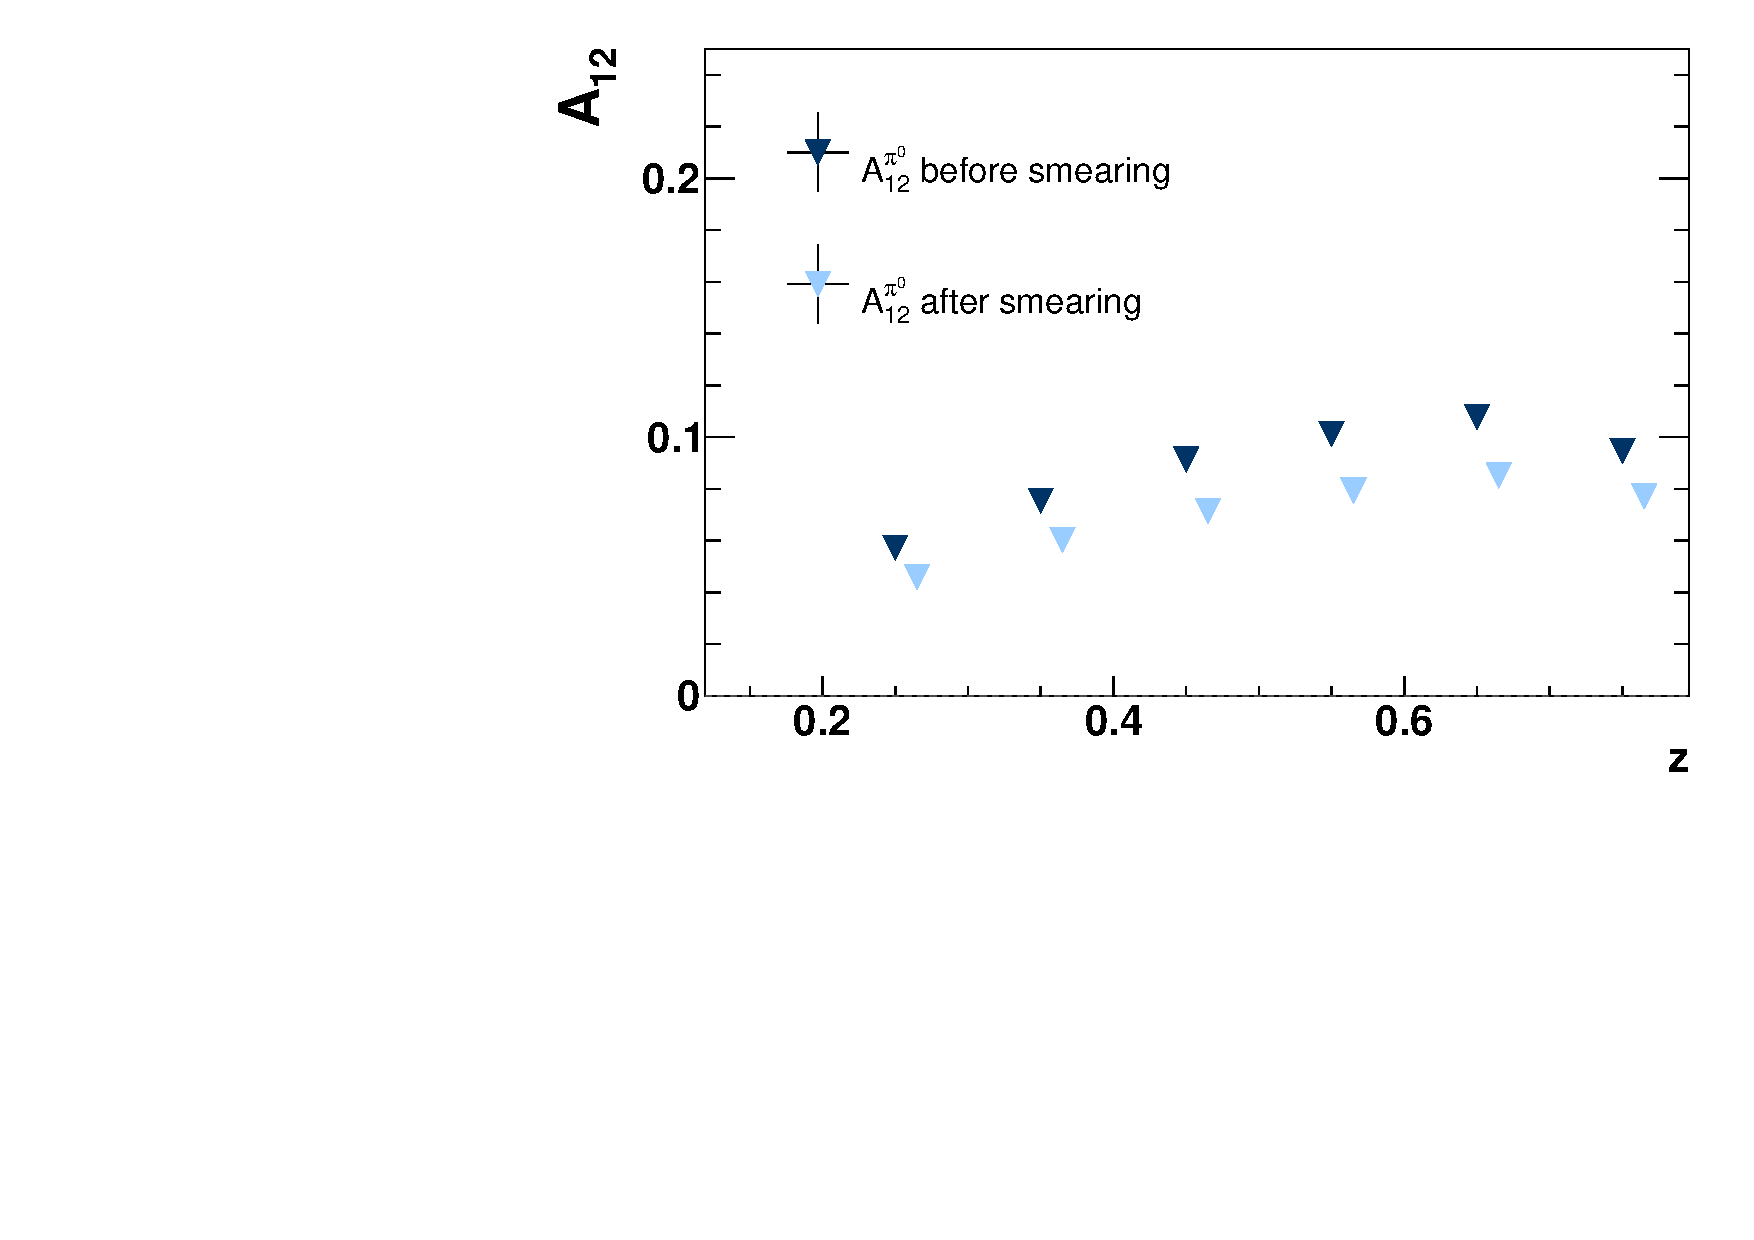
\includegraphics[width=.48\textwidth,natwidth=600,natheight=400]{figure_asy/corrections/before&after_smearing0.pdf}}
  \subfigure[$P_{t1}$ bins]{\label{fig:weightpi02}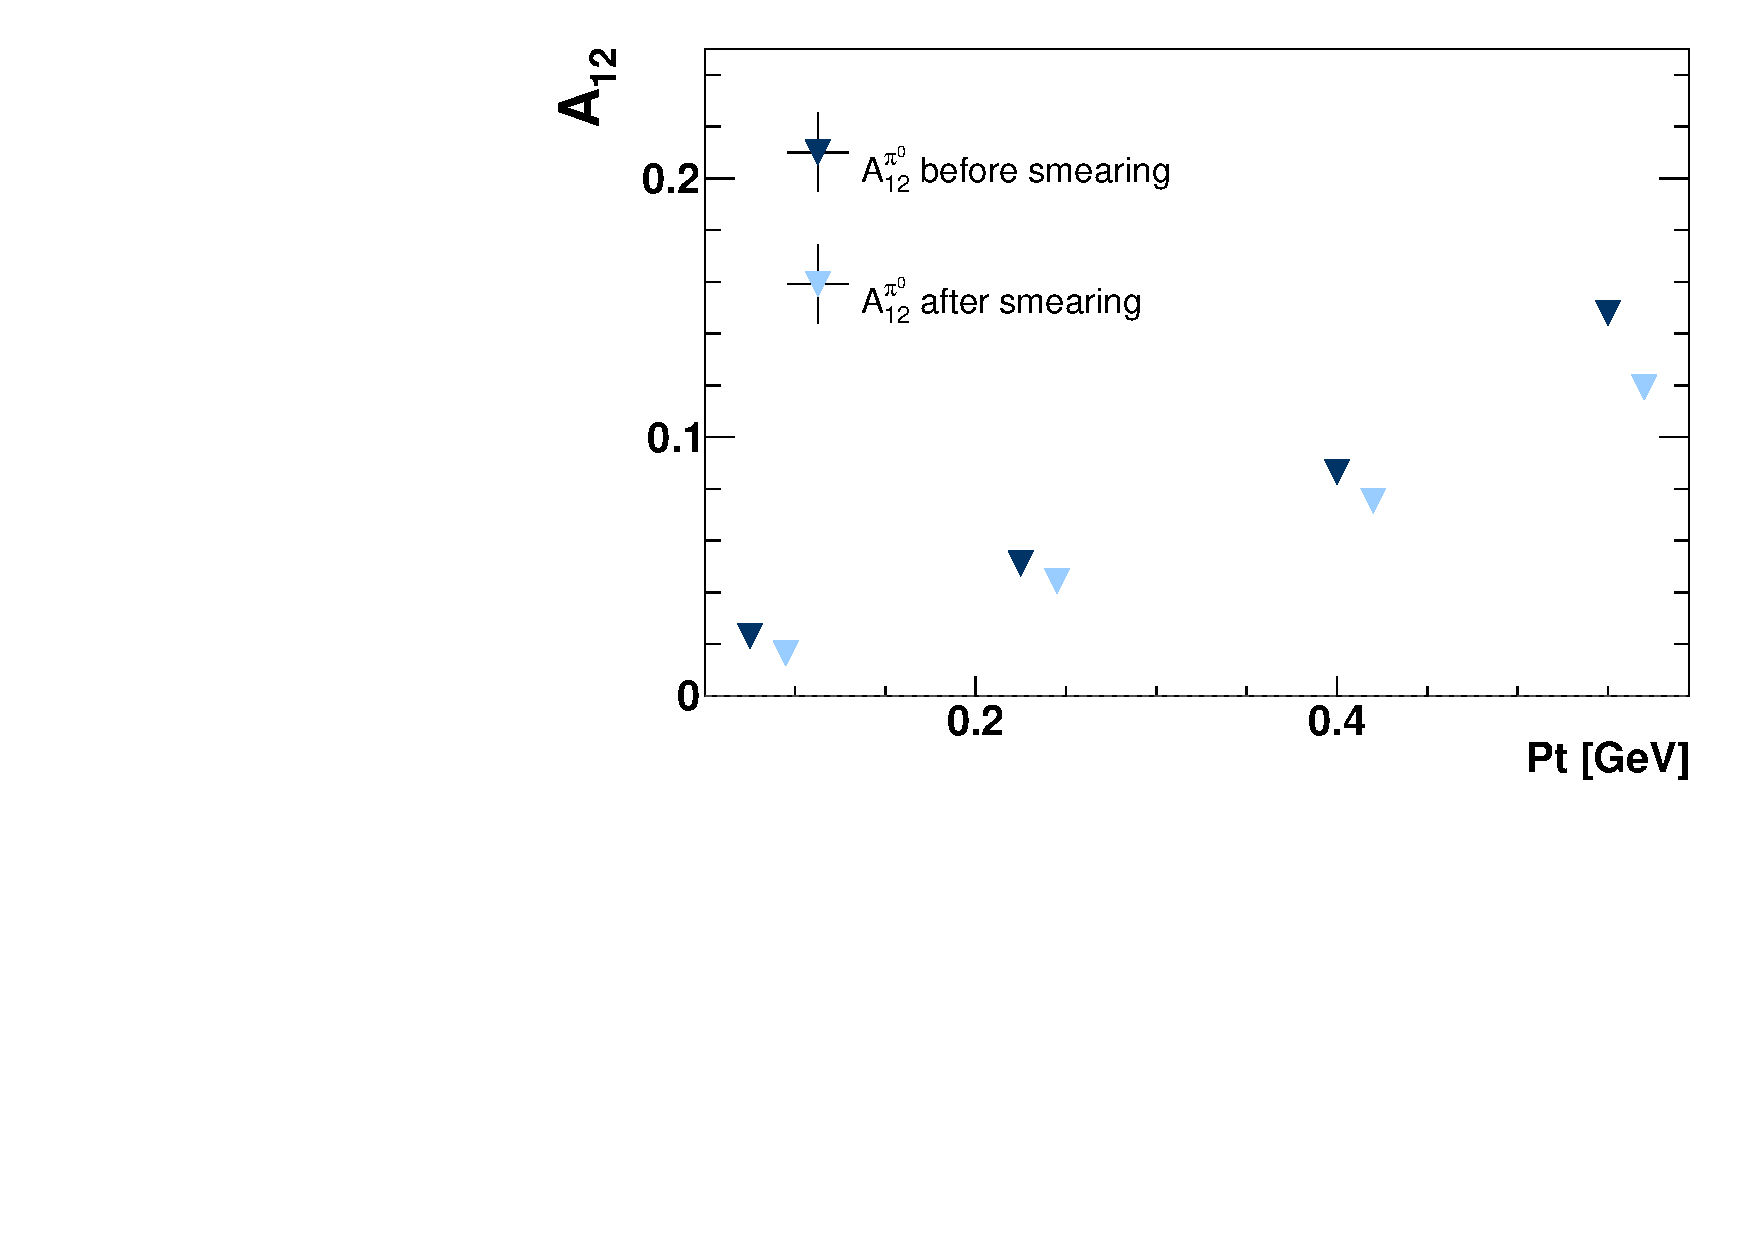
\includegraphics[width=.48\textwidth,natwidth=600,natheight=400]{figure_asy/corrections/before&after_smearing2.pdf}}
  \subfigure[$(z_1,z_2)$ bins]{\label{fig:weightpi03}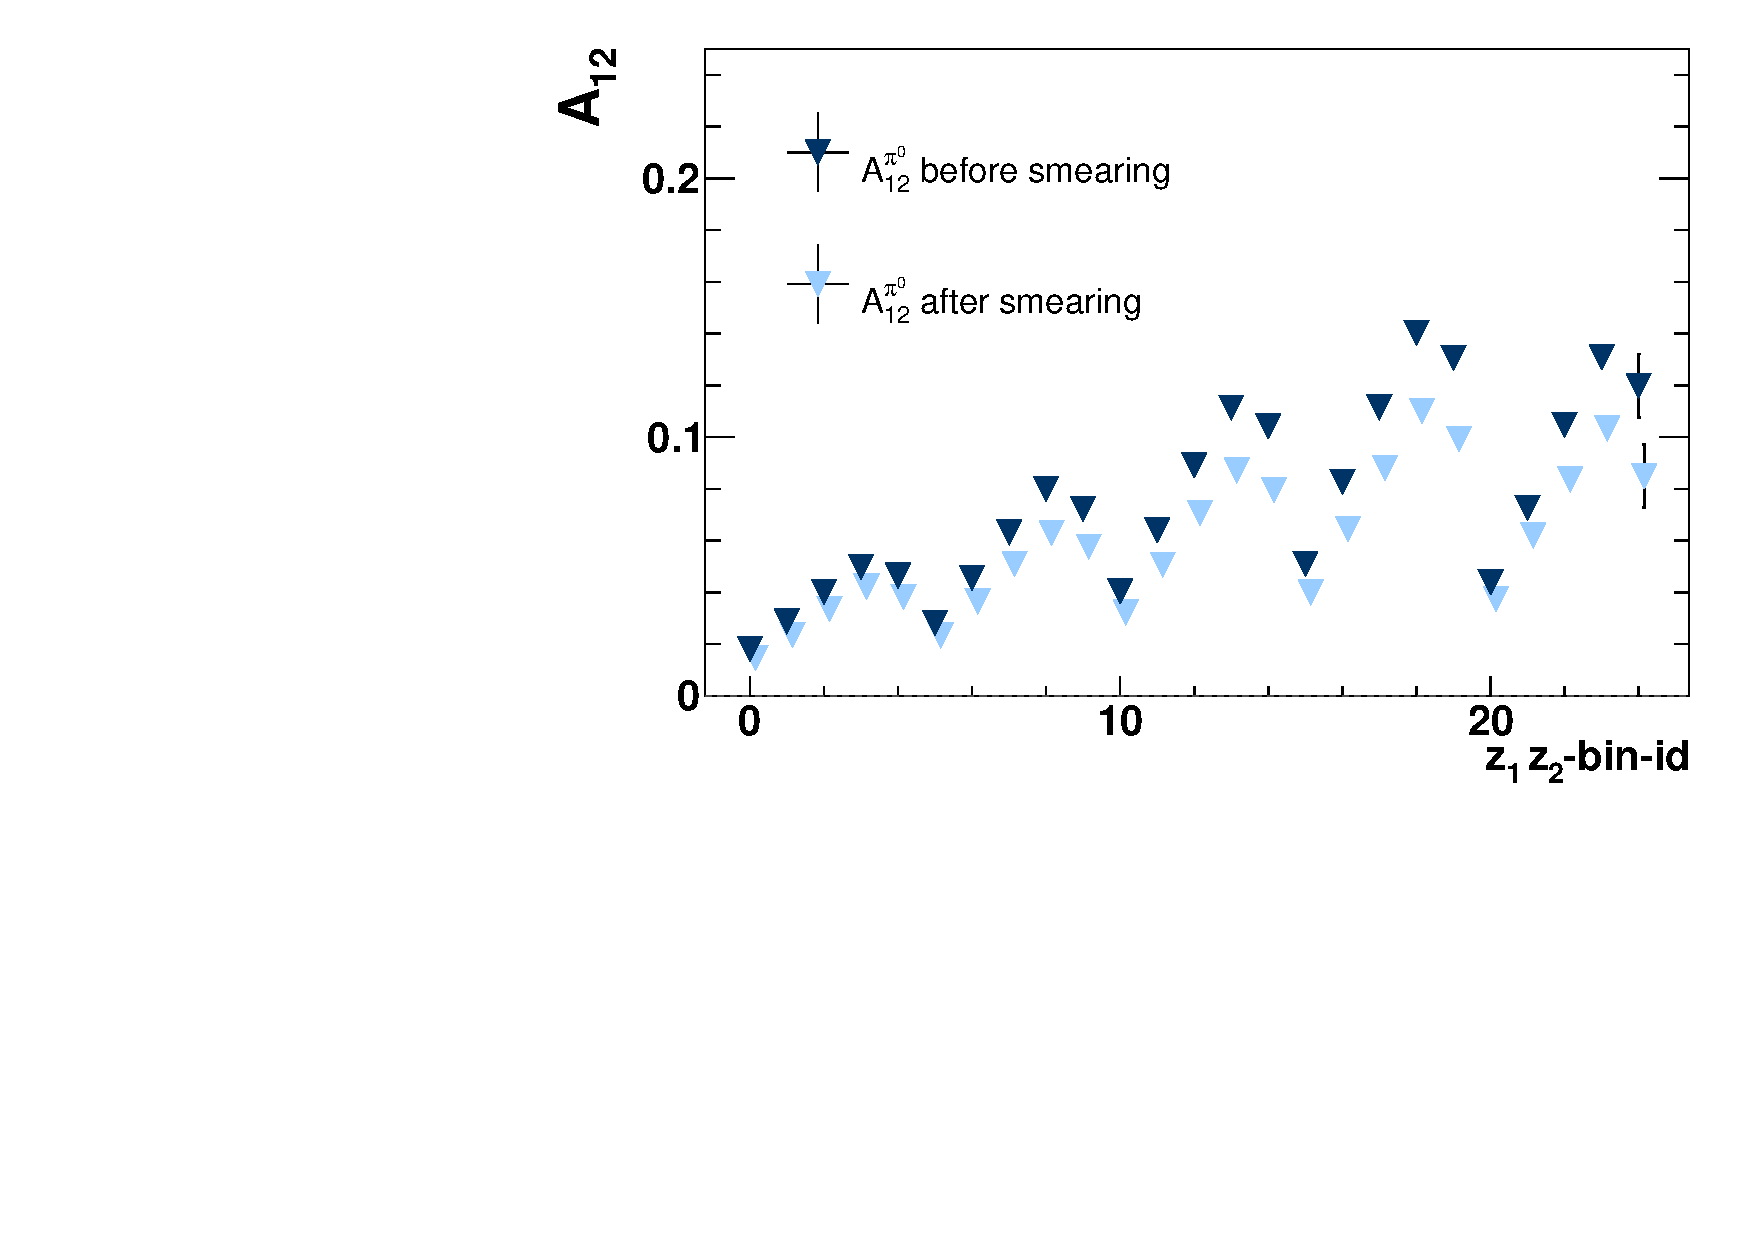
\includegraphics[width=.48\textwidth,natwidth=600,natheight=400]{figure_asy/corrections/before&after_smearing1.pdf}}
  \subfigure[$(P_{t1},P_{t2})$ bins]{\label{fig:weightpi04}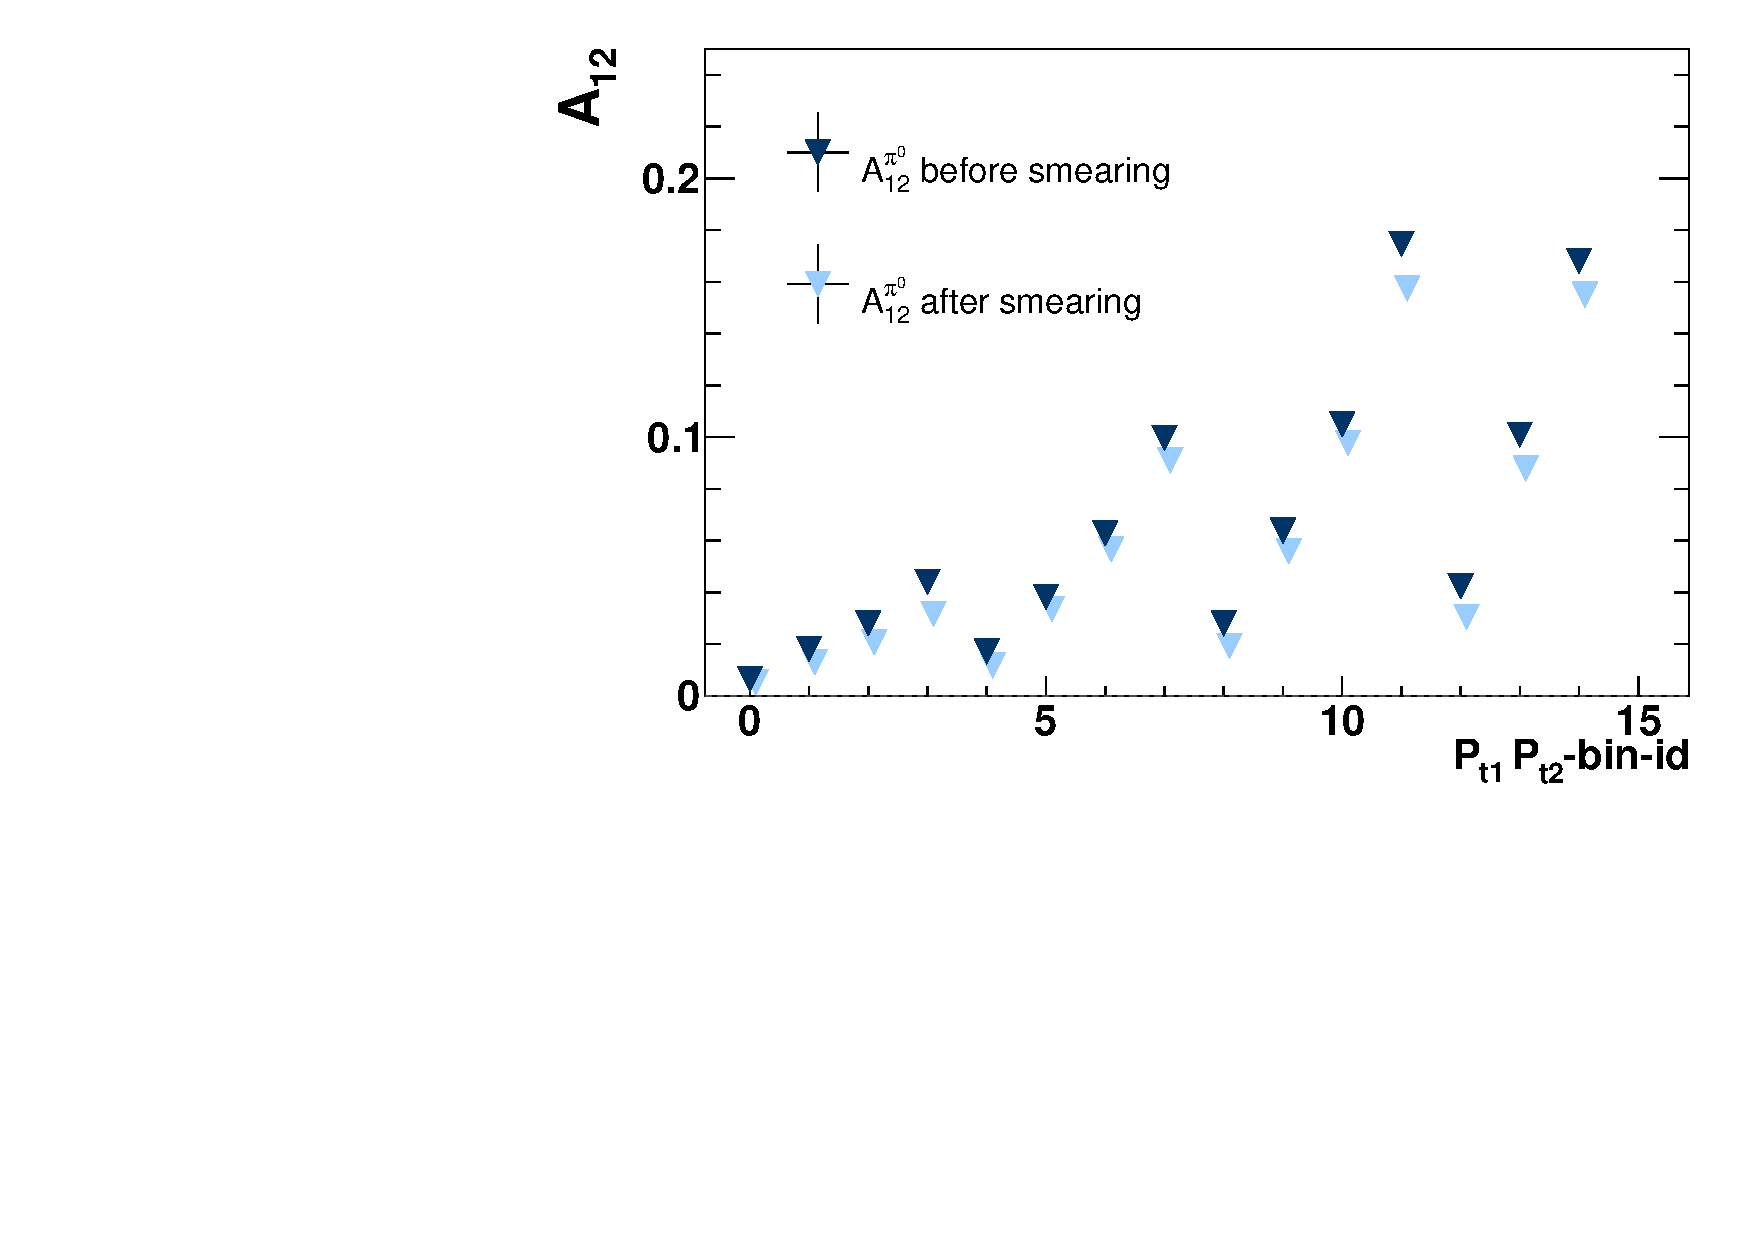
\includegraphics[width=.48\textwidth,natwidth=600,natheight=400]{figure_asy/corrections/before&after_smearing3.pdf}}
  \caption[Weighted $\pi^0$ double-ratio asymmetries $\nicefrac{A^{0\pm}_{12}}{A^L_{12}}$]{Weighted $\pi^0$ double-ratio asymmetries $\nicefrac{A^{0\pm}_{12}}{A^L_{12}}$. As described in the text, the weight for the numerator  $\pi^0\pi^++\pi^0\pi^-$ is $1\times P_{t1}P_{t2}$ while the weight for the denominator $\pi^+\pi^++\pi^-\pi^- $ is $0.25\times P_{t1}P_{t2}$.}
  \label{fig:weightpi0}
\end{figure}



  Here, the theoretical value $A_{i}$ is chosen as a function of $P_T$ with a functional shape such that the reconstructed asymmetries (after smearing) closely resemble the measured physics asymmetries.
We adopted  a weight $1*P_{t1}*P_{t2}$ for the hadrons in the numerator and $0.25*P_{t1}*P_{t2}$ for hadrons in the denominator of the double ratio (the weight factor 0.25 for the denominator is chosen to
give the smeared asymmetries as observed in the data). 
Since we measure double ratios, we can scale the weights in the numerator and denominator to achieve the same measured asymmetry. We tried a relative scaling of up to a factor 5 and 
the difference in the resulting correction factors was negligible compared with their statistical uncertainties.
 The output based on the {\em measured-thrust} is the smeared asymmetry and the output asymmetry based on the {\em stable-thrust} is the real asymmetry that we manually generated. The ratio between those two is the smearing-correction factor, to be applied to the asymmetries measured using real data.
 
 % We observe a significant dilution of the reconstructed asymmetries and the value $\nicefrac{A_{inject}}{A_{measured}}$ represents the thrust smearing factor. 

 %By using the constant injection asymmetry as the weight 0.1 we mentioned above, we can only get an raw estimation of smearing factor. A constant injection implies that all events contribute the same weight to the smearing effect, however the events that are close to thrust axis usually smeared most. Moreover, those events generally belong to low $P_t$ range and carry small Collins effect. By assigning the same weight to all events, we may overvalue those events and wrongly estimate the smearing effect. To solve this problem, a $P_t$ dependent weight,  for example $a*P_{t1}*P_{t2}$ , can be applied. 
 

%The disadvantage of direct measurement is that the statistics of Belle MC would lead to uncertainty which is hard to determine. For most bins, the statistic uncertainty is about few percent of the asymmetry and other uncertainties would dominate. %Therefore we neglect the statistic uncertainty in this method. Theoretically the regenerated method, on the other hand, has none statistical uncertainty as we can generate as much data as we need. But it can only predict the smearing effect imprecisely. Hence, we use the regenerate method as a cross check and the re-weighting result will be used for correction.

\subsubsection{Average Injected Weight}
In the last section, we used the weight $1*P_{t1}*P_{t2}$ for the numerator and $0.25*P_{t1}*P_{t2}$ for the denominator to simulate the asymmetry. To better serve the purpose of theoretical study, here we list the average value of the injected weight together with the other information for the smearing correction. Details for other kinematic bins can be found in \ref{sec:appendixC}.
\begin{table}[H]\footnotesize
\centering
\begin{tabular}{|l|l|l|l|l|l|l|l|l|l|l|l|l|l|l|l|l|l|}
\hline
$z_1$ bins & $A_{stable}$ & $\delta A_{stable}$ & Average Weight &  $A_{measured}$ & factor  & Uncertainty\\ \hline
0	&		&		&		&		&		&		\\ \hline
1	&	0.0572	&	0.0002	&	0.0582	&	0.0460	&	1.245	&	0.005	\\ \hline
2	&	0.0754	&	0.0003	&	0.0769	&	0.0601	&	1.255	&	0.005	\\ \hline
3	&	0.0913	&	0.0004	&	0.0907	&	0.0714	&	1.278	&	0.006	\\ \hline
4	&	0.1013	&	0.0006	&	0.1001	&	0.0793	&	1.278	&	0.008	\\ \hline
5	&	0.1077	&	0.0010	&	0.1042	&	0.0852	&	1.264	&	0.012	\\ \hline
6	&	0.0947	&	0.0015	&	0.0900	&	0.0773	&	1.226	&	0.020	\\ \hline
\end{tabular}
\caption[Various values used in the smearing correction]{Values used in the smearing correction analysis. $A_\textrm{stable}$ is the asymmetry for that bin, measured using the correct 
(stable) thrust axis, while $A_\textrm{measured}$ uses the reconstructed 
(e.g., smeared) thrust axis. The Average Weight gives the average of 
the event-wise weights for a given bin.
\label{tab:sinz_smearing_info}}
\end{table}

\iffalse
\subsubsection{\texorpdfstring{Regenerate Smearing Effect}{Regenerated Smearing Effect}} 
\label{sec:regeneratedsmearing}
The thrust axis shift effect both the inaccurate measurement of Collins angle and transverse momentum $P_t$. Here we use two steps procedure to simulate these effects separately.

The resolution of Collins angle, defined as the difference between real and measured Collins angle Eq.~\ref{eqn:CollinsAngleReso}, could be parameterized and used to regenerate the Collins angle smearing effect. 

\begin{equation}
\Delta\phi_{12}=|\phi_{12}^{\text{real}}-\phi_{12}^{\text{measure}}|
\label{eqn:CollinsAngleReso}
\end{equation}

\begin{figure}[H]
  \centering     
  \subfigure[Collins angle resolution of $z_1$ bins 1, $\pi^0\pi^-$ pairs]{\label{fig:shift1}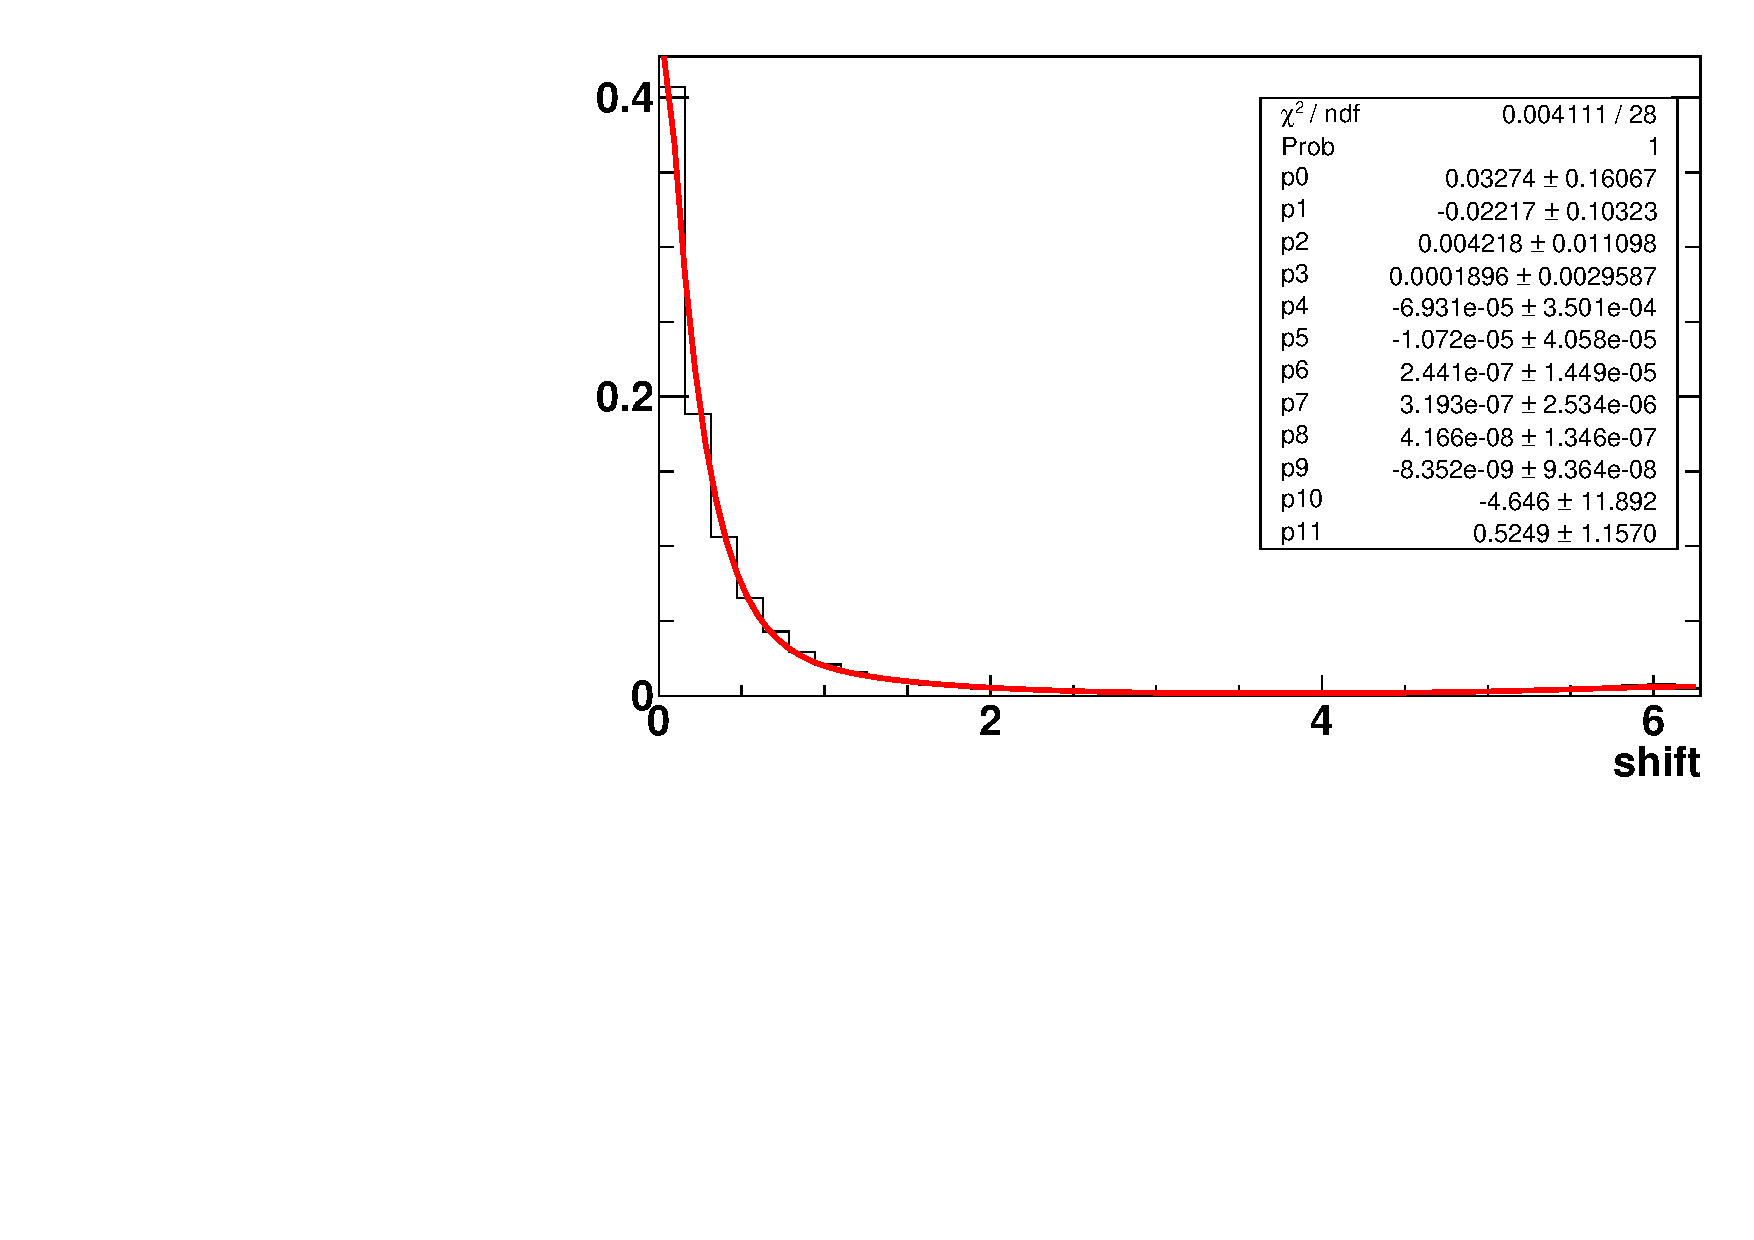
\includegraphics[width=60mm,natwidth=600,natheight=400]{figure_asy/corrections/Phi12pipi0NSinZ1_shift_fit.pdf}}
  \subfigure[Collins angle resolution of $z_1$ bins 5, $\pi^0\pi^-$ pairs]{\label{fig:shift2}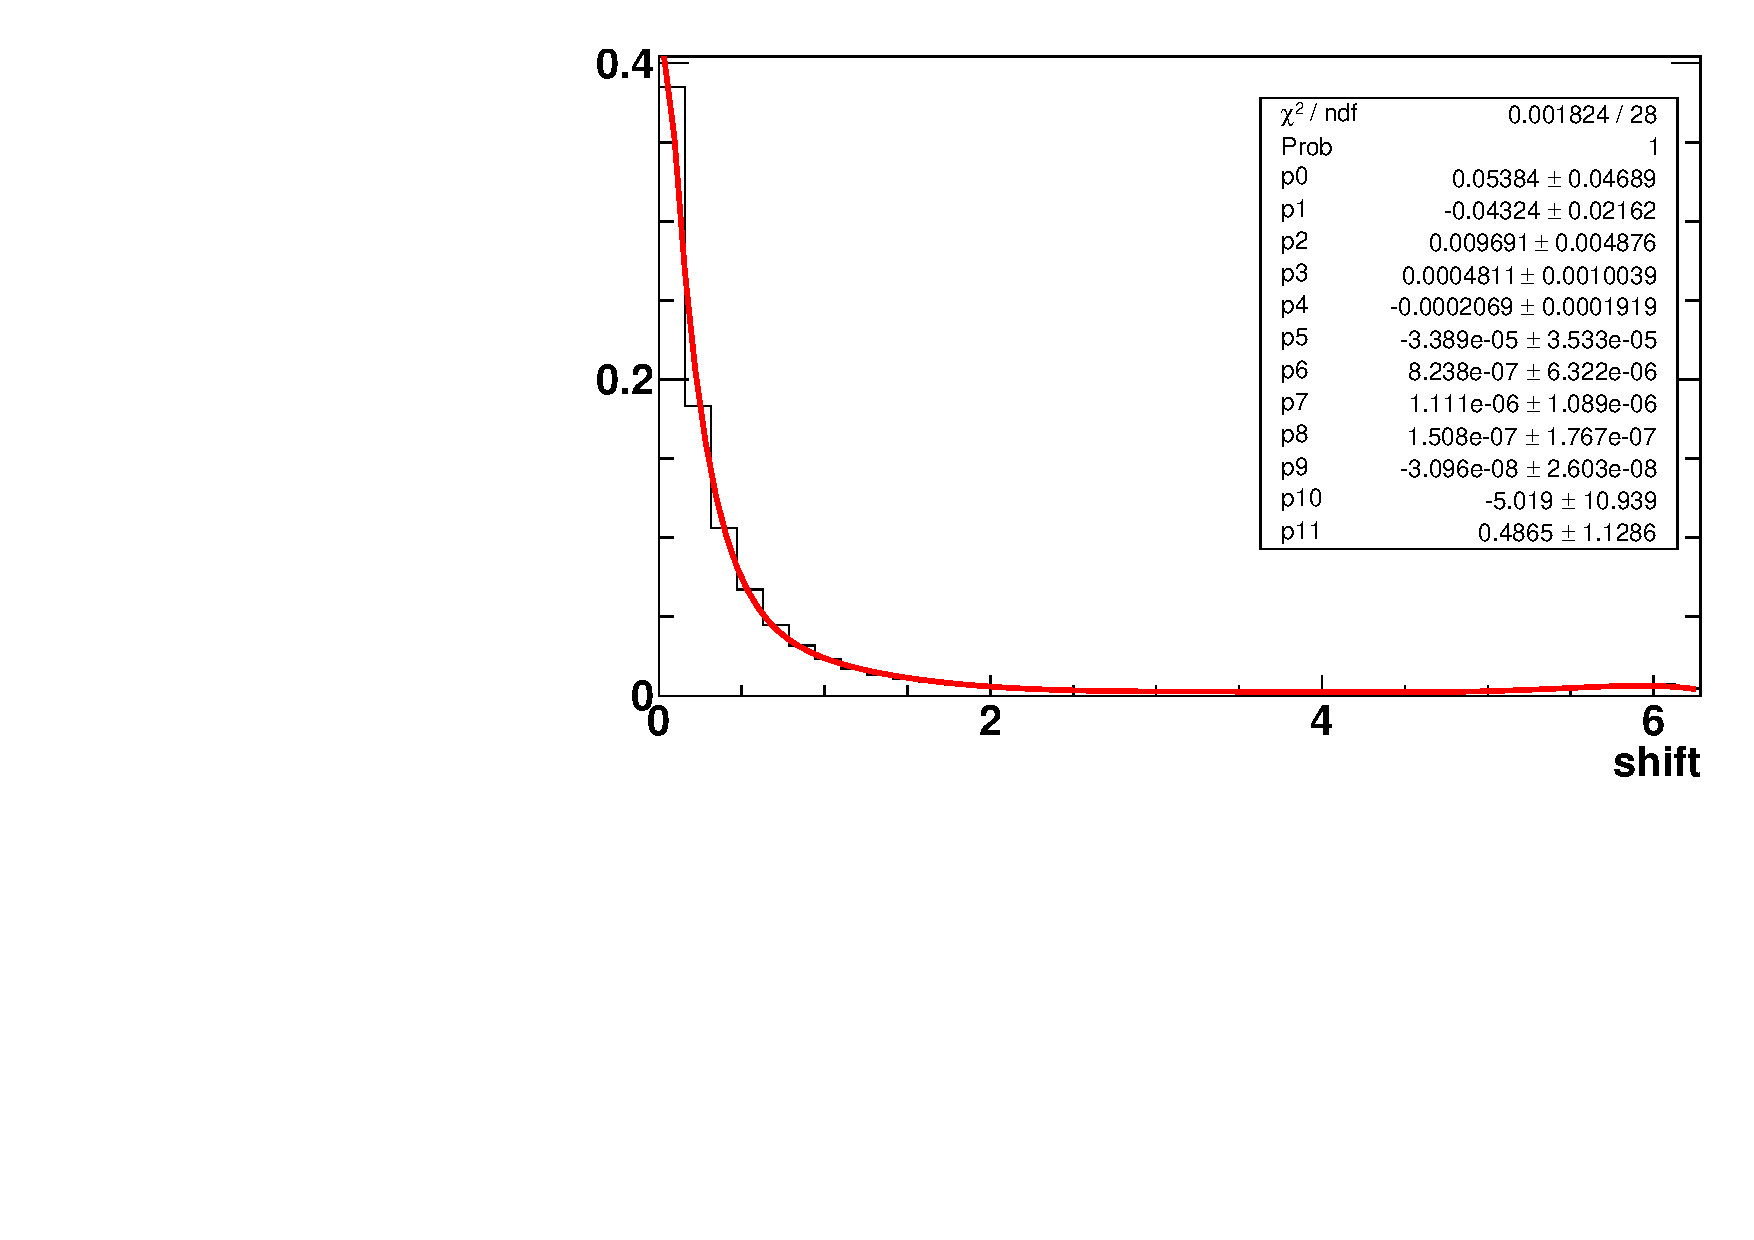
\includegraphics[width=60mm,natwidth=600,natheight=400]{figure_asy/corrections/Phi12pipi0NSinZ5_shift_fit.pdf}}
  \subfigure[Collins angle resolution of $P_{t1}$ bins 0, $\pi^0\pi^-$ pairs]{\label{fig:shift3}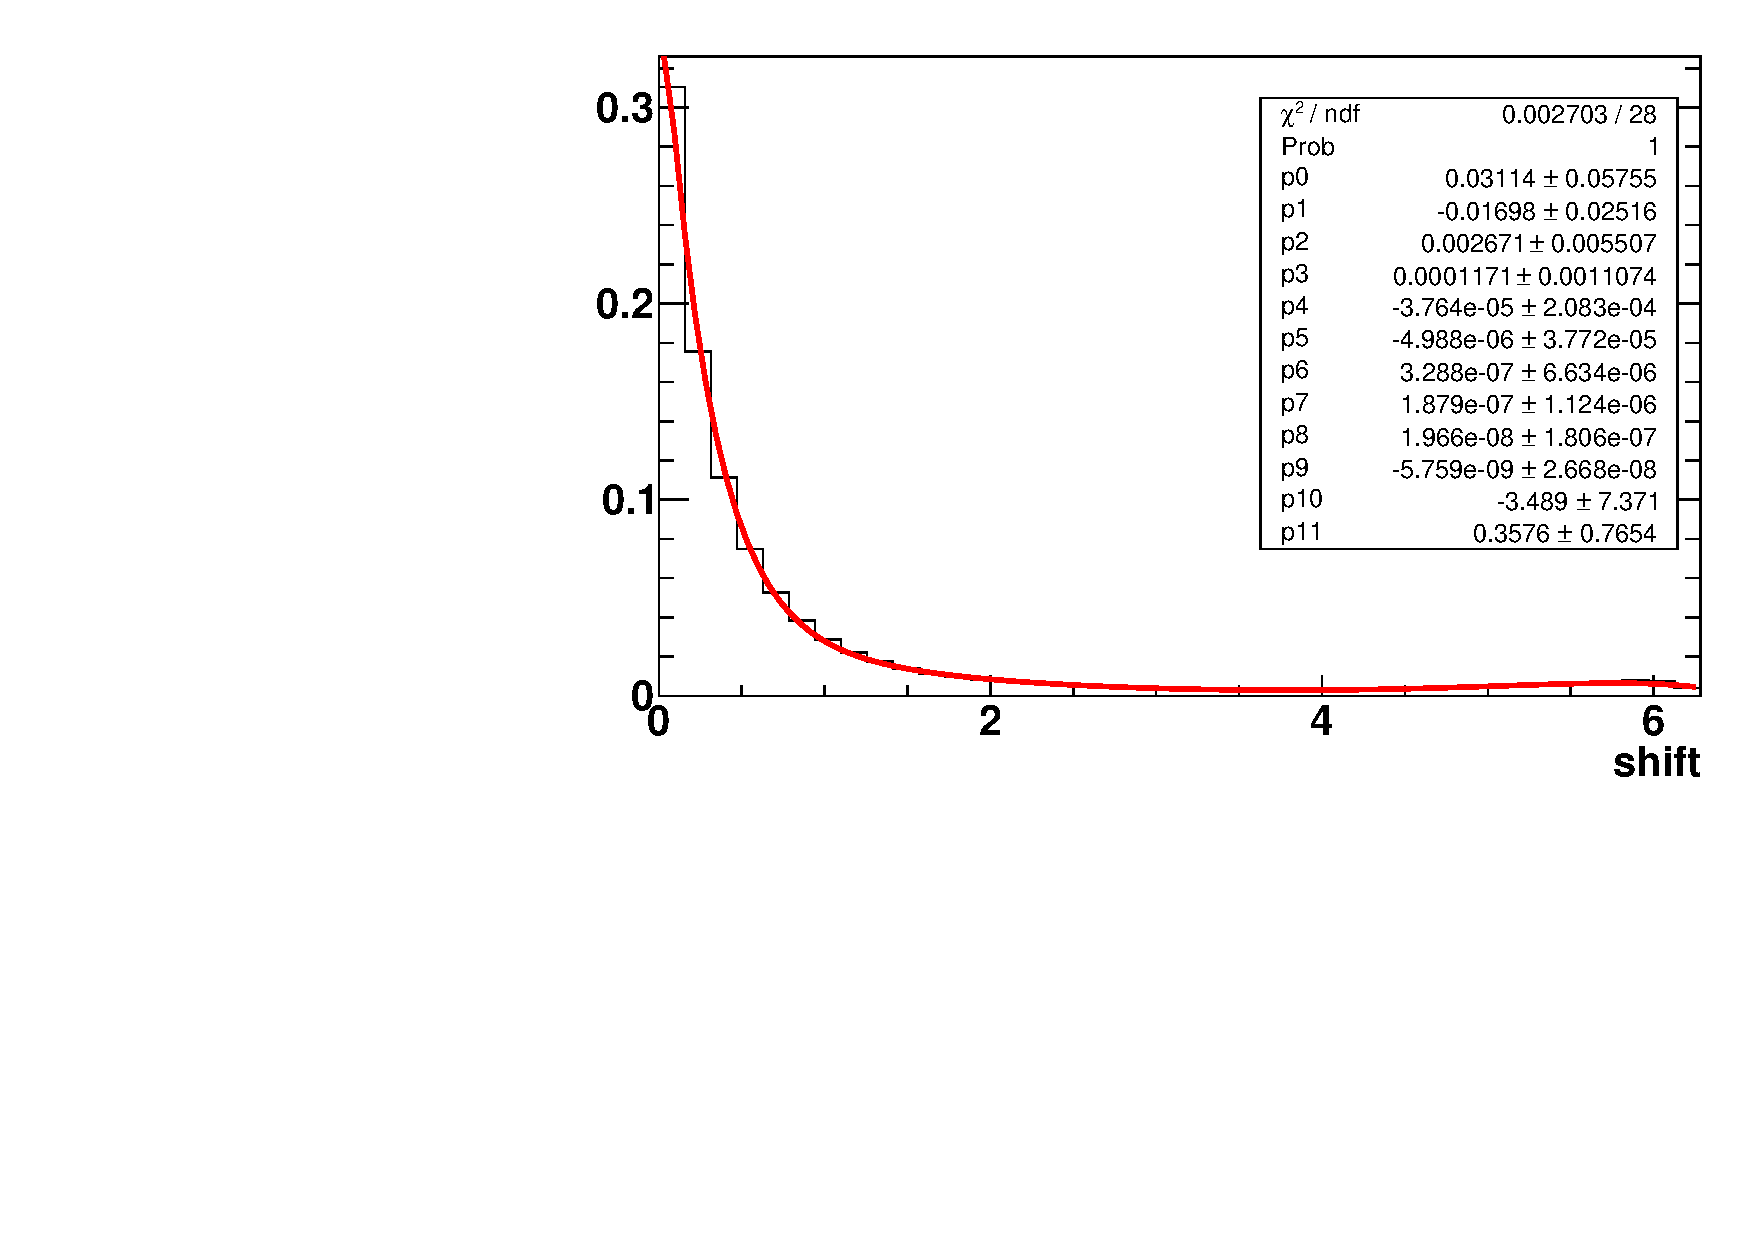
\includegraphics[width=60mm,natwidth=600,natheight=400]{figure_asy/corrections/Phi12pipi0NSinPt0_shift_fit.pdf}}
  \subfigure[Collins angle resolution of $P_{t1}$ bins 3, $\pi^0\pi^+$ pairs]{\label{fig:shift4}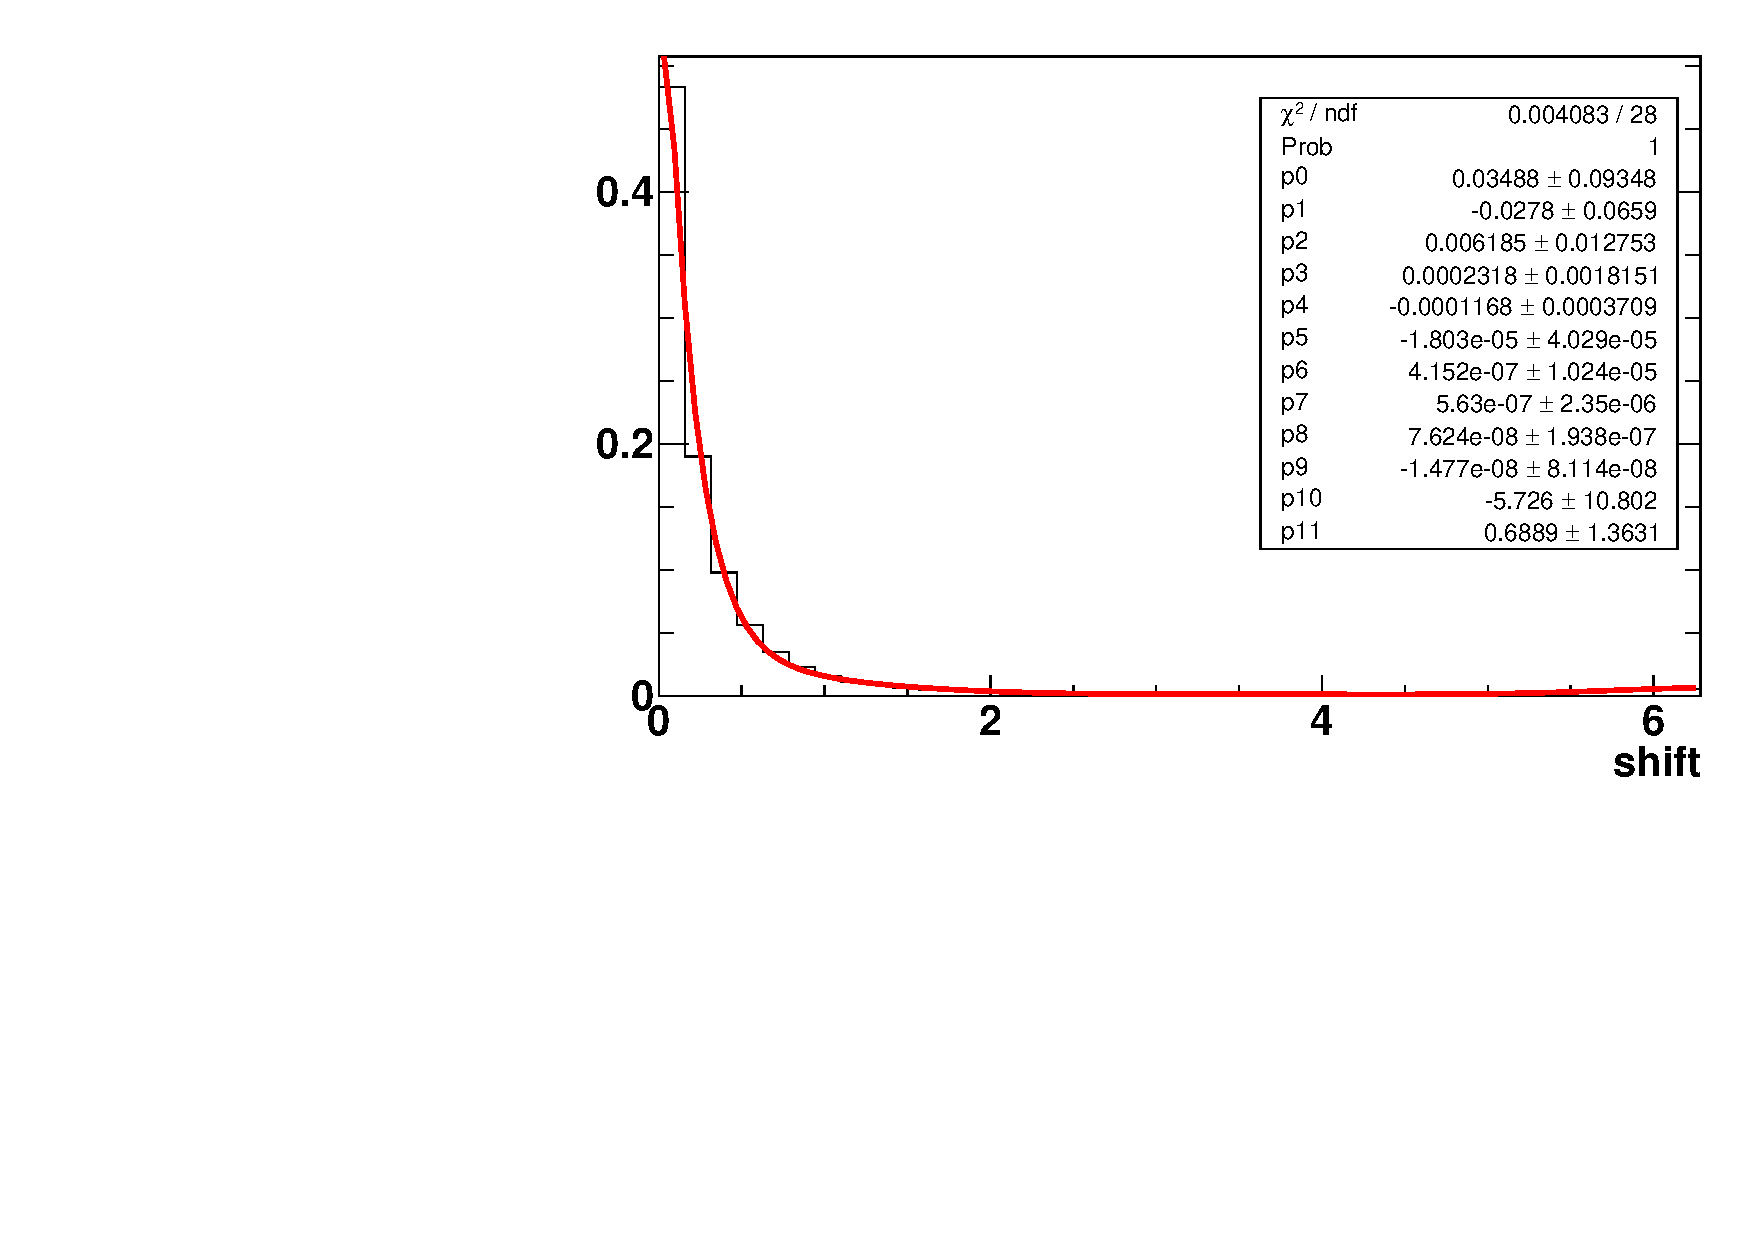
\includegraphics[width=60mm,natwidth=600,natheight=400]{figure_asy/corrections/Phi12pipi0NSinPt3_shift_fit.pdf}}
  \caption{Collins angle resolution of pion hadron pairs. The resolution is fitted with polynomial function.}
  \label{fig:shift}
\end{figure}
In Fig.~\ref{fig:shift3} the tails of resolution of lower $P_t$ bins are wider, which indicates higher smearing correction. The resolution functions for different hadron pairs is plotted in Fig.~\ref{fig:shiftcompare}. It can be seen that the resolution function of different hadron types that are contained in one double ratio are almost identical. This is consistent with the matching kinematic distribution of hadrons that we discussed in section~\ref{sec:fiducialcut}.

\begin{figure}[H]
  \centering     
  \subfigure[resolution of $(z_1,z_2)$ bins 1, $\pi^0$ pairs]{\label{fig:shiftcompare1}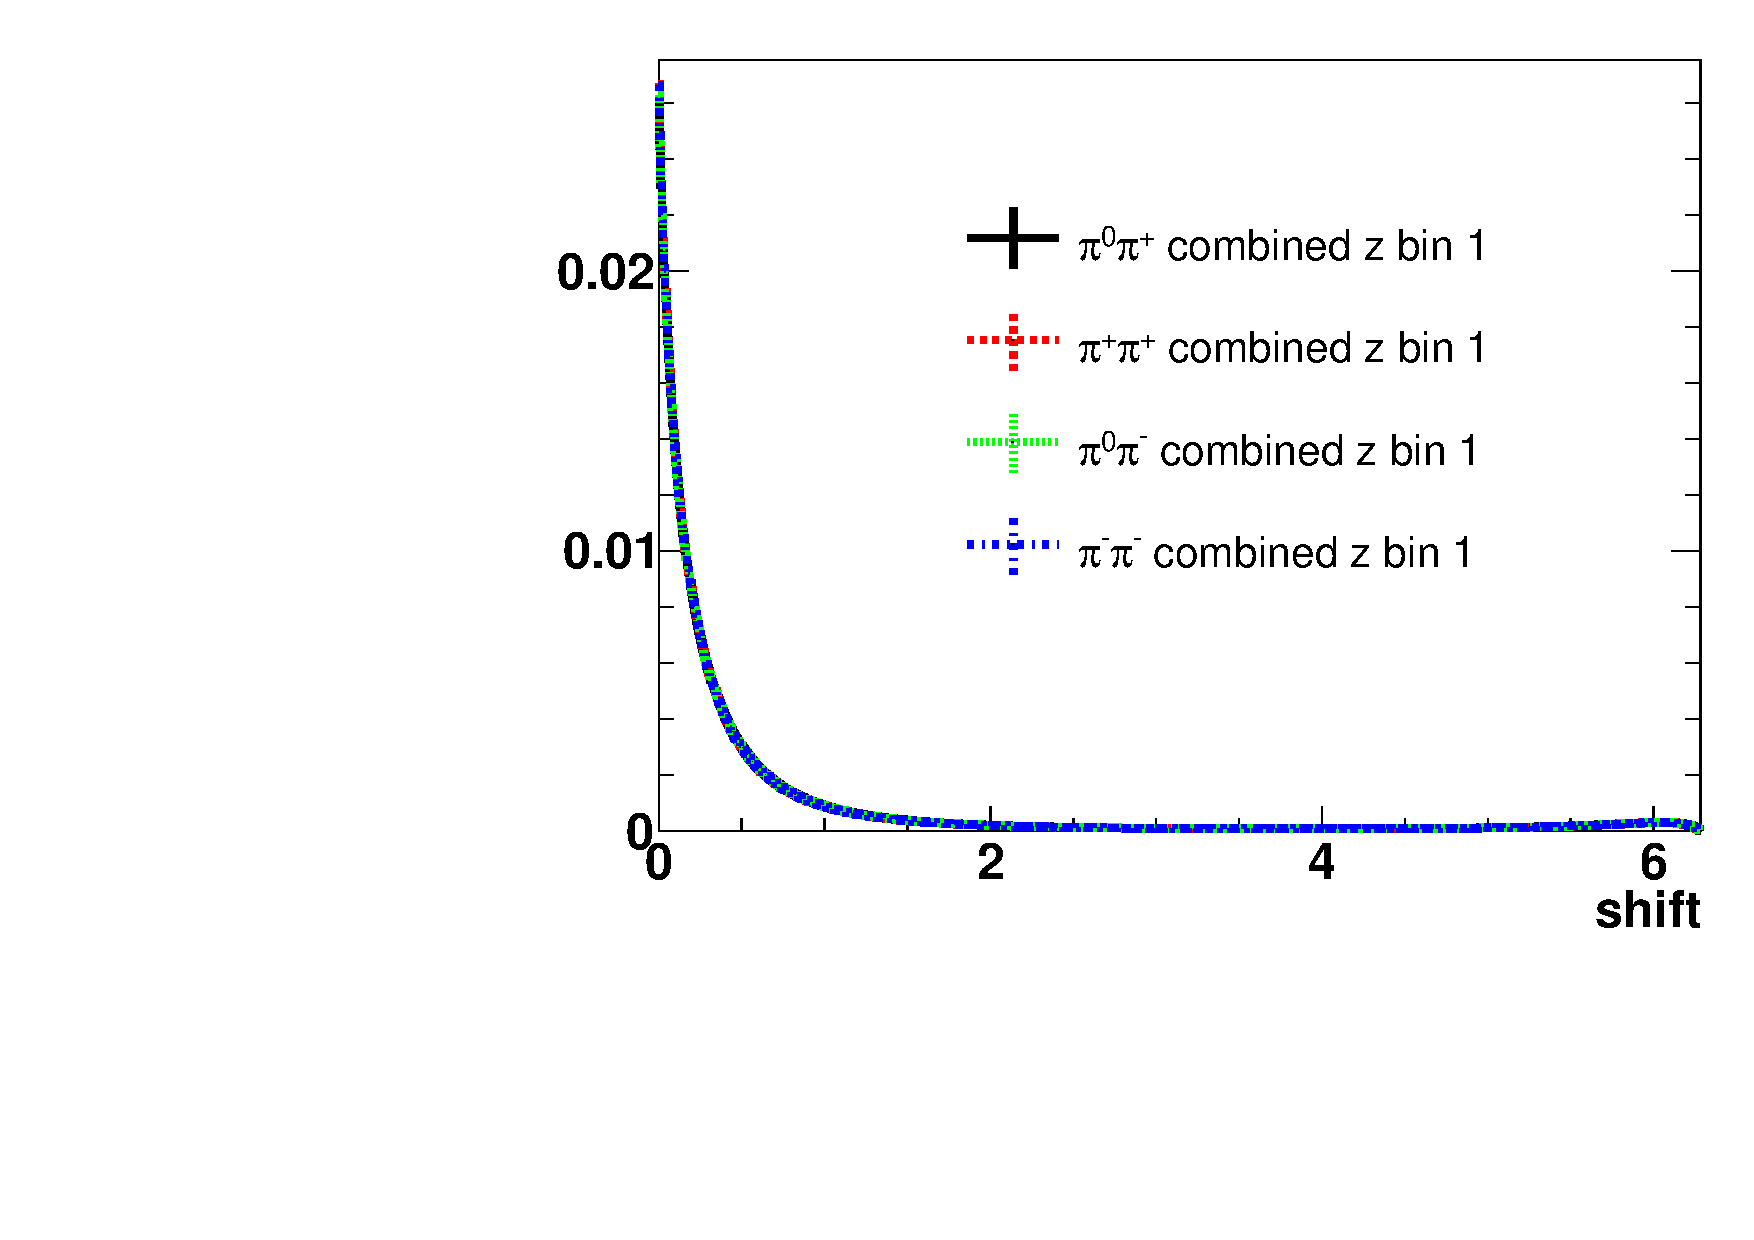
\includegraphics[width=60mm,natwidth=600,natheight=400]{figure_asy/corrections/pi0pairs_shift_compare_ComZ_1.pdf}}
  \subfigure[resolution of $(z_1,z_2)$ bins 8, $\pi^0$ pairs]{\label{fig:shiftcompare2}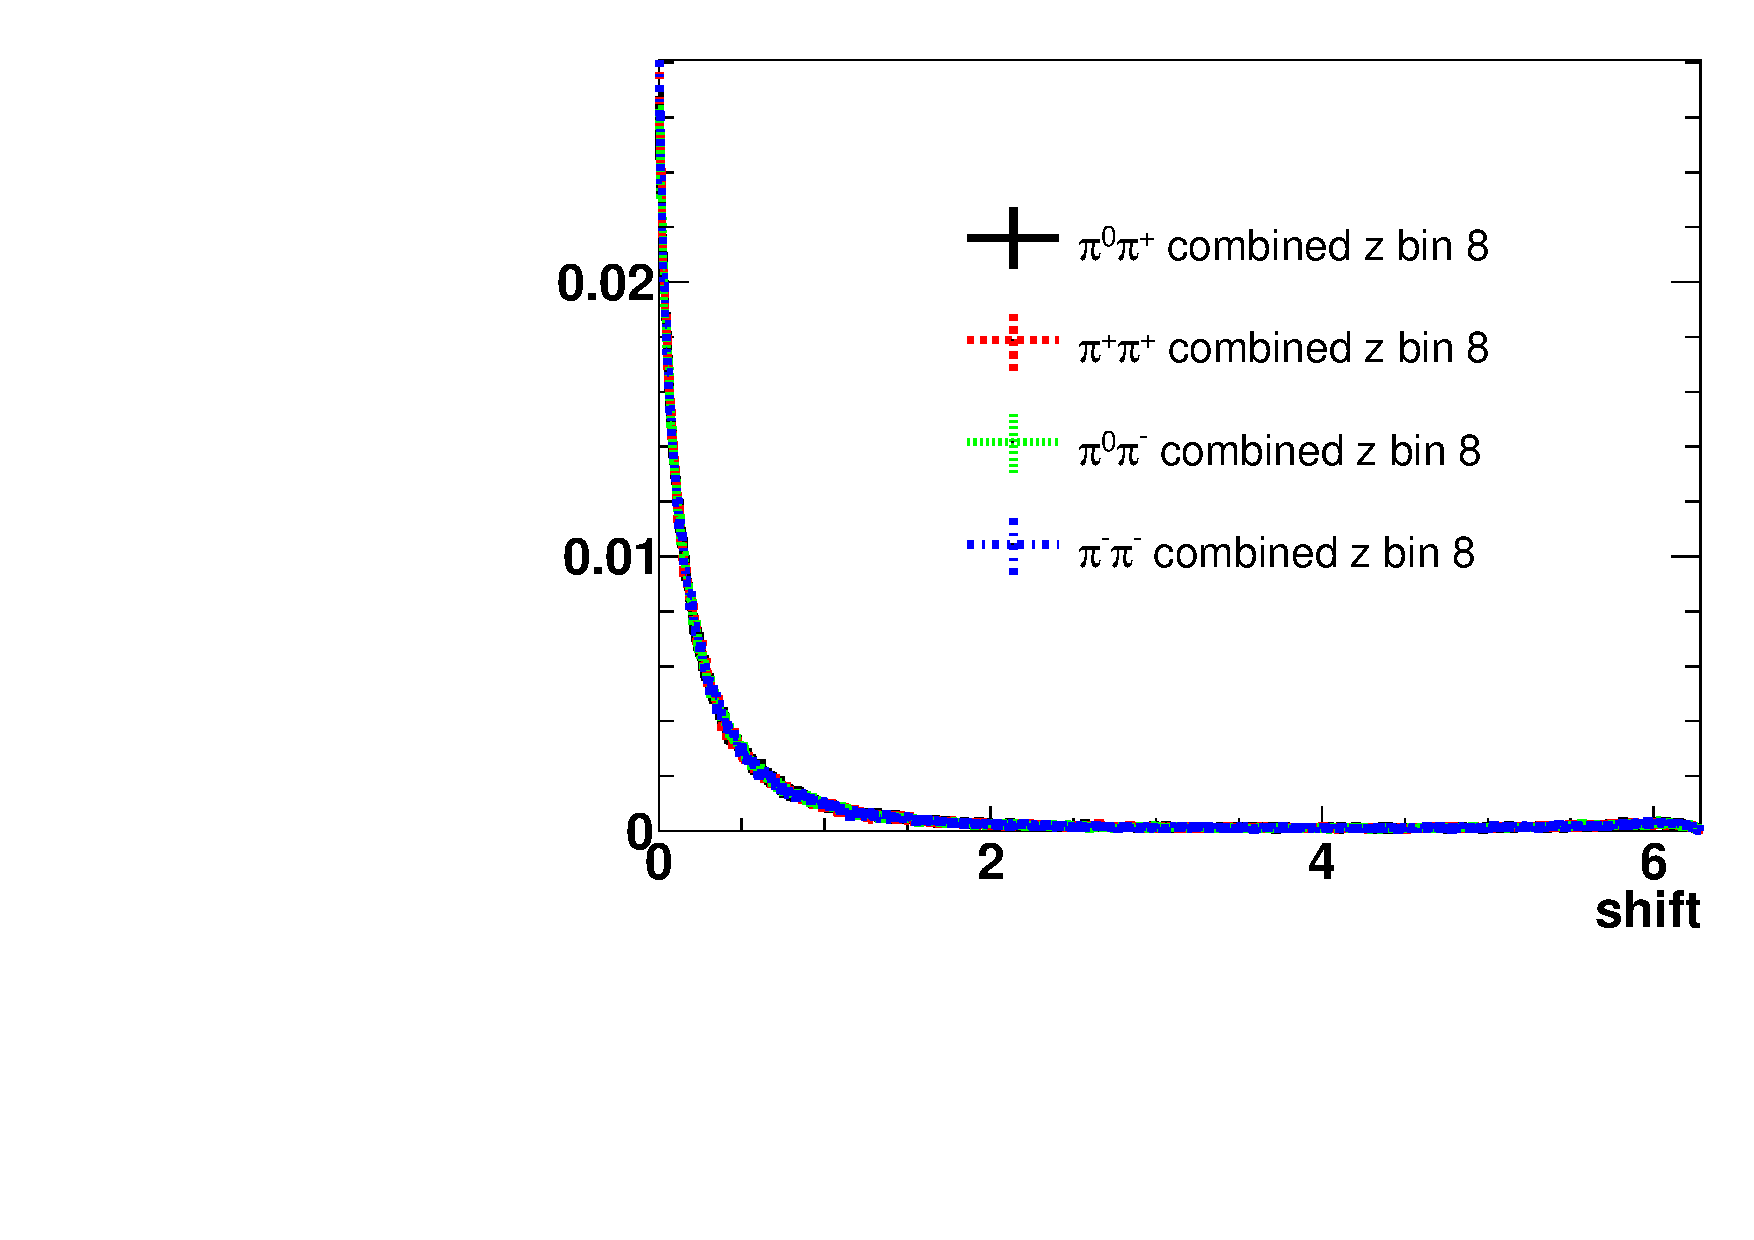
\includegraphics[width=60mm,natwidth=600,natheight=400]{figure_asy/corrections/pi0pairs_shift_compare_ComZ_8.pdf}}
  \subfigure[resolution of $(z_1,z_2)$ bins 4, $\eta$ pairs]{\label{fig:shiftcompare1}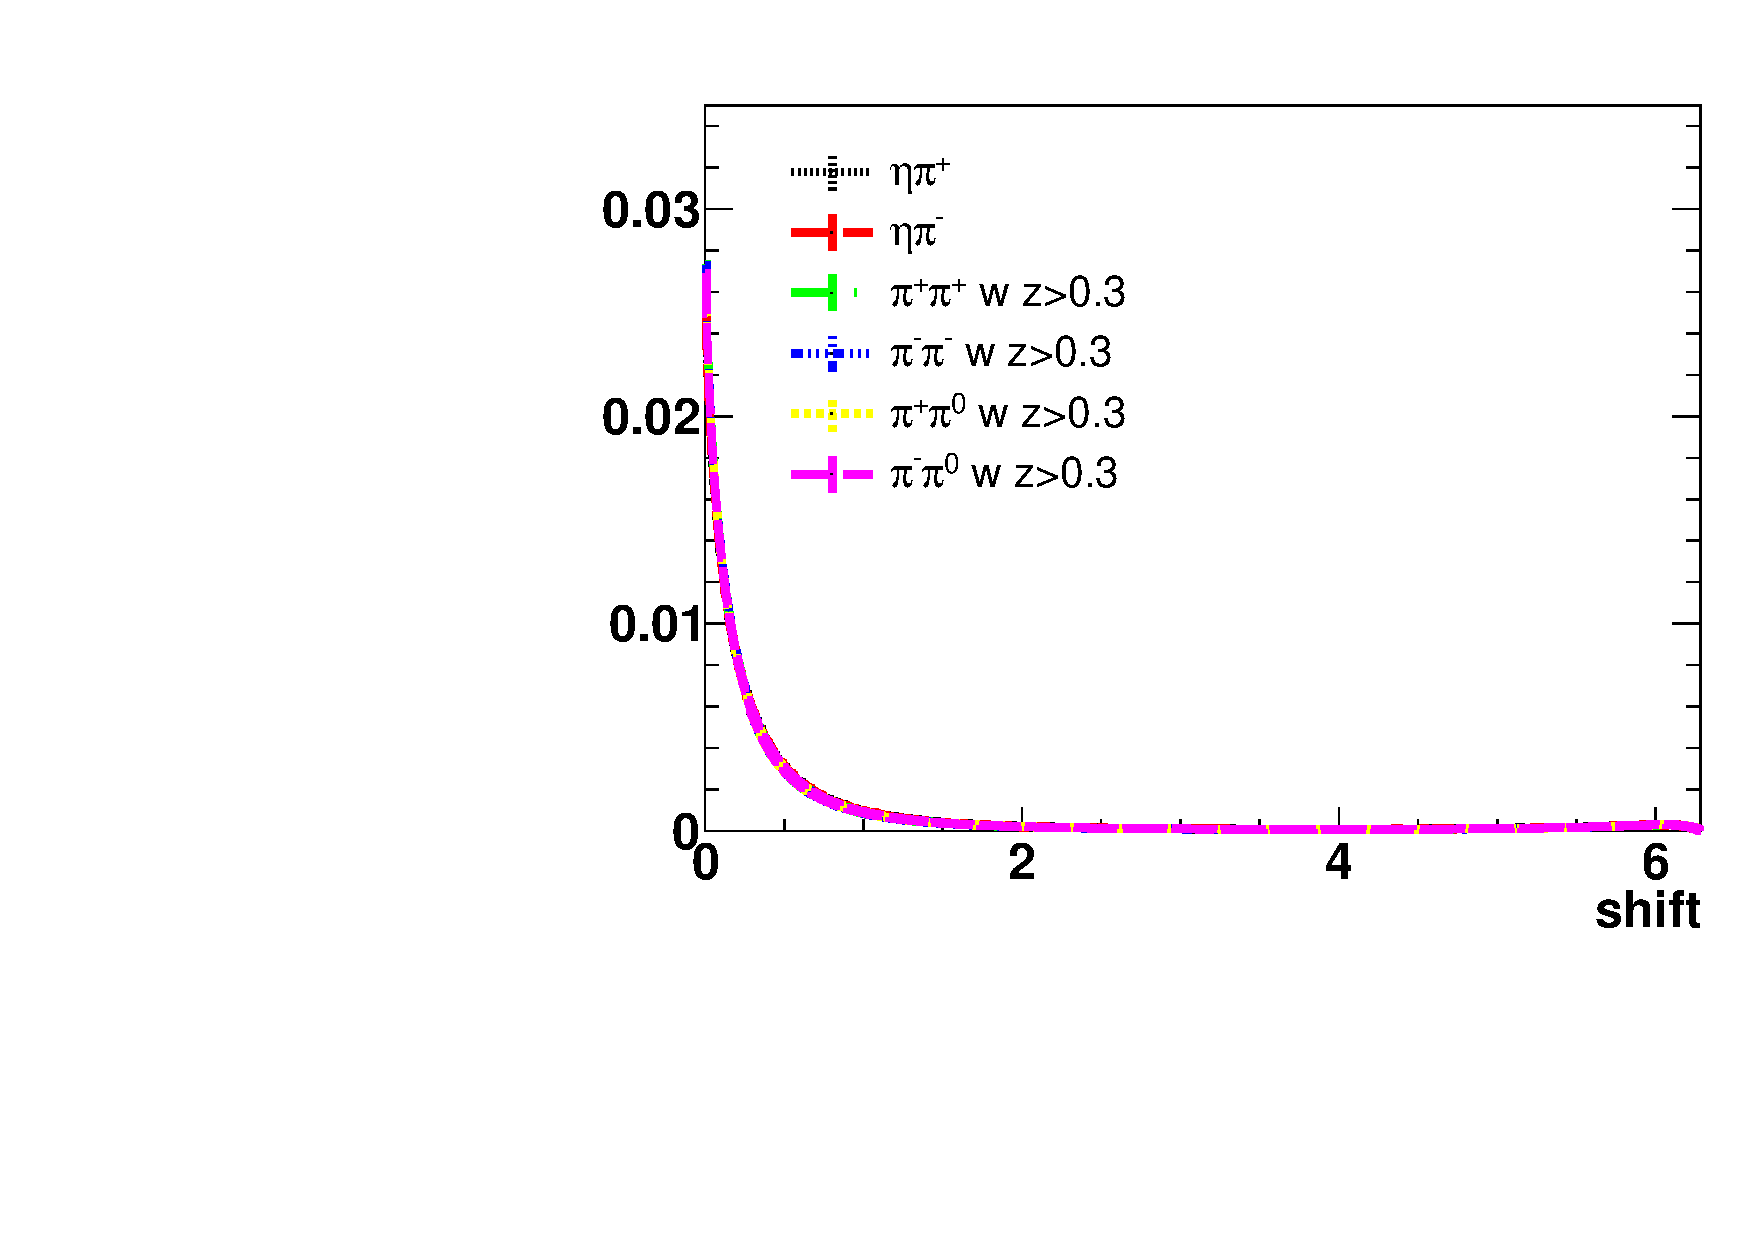
\includegraphics[width=60mm,natwidth=600,natheight=400]{figure_asy/corrections/etapairs_shift_compare_ComZ_4.pdf}}
  \subfigure[resolution of $(z_1,z_2)$ bins 8, $\eta$ pairs]{\label{fig:shiftcompare2}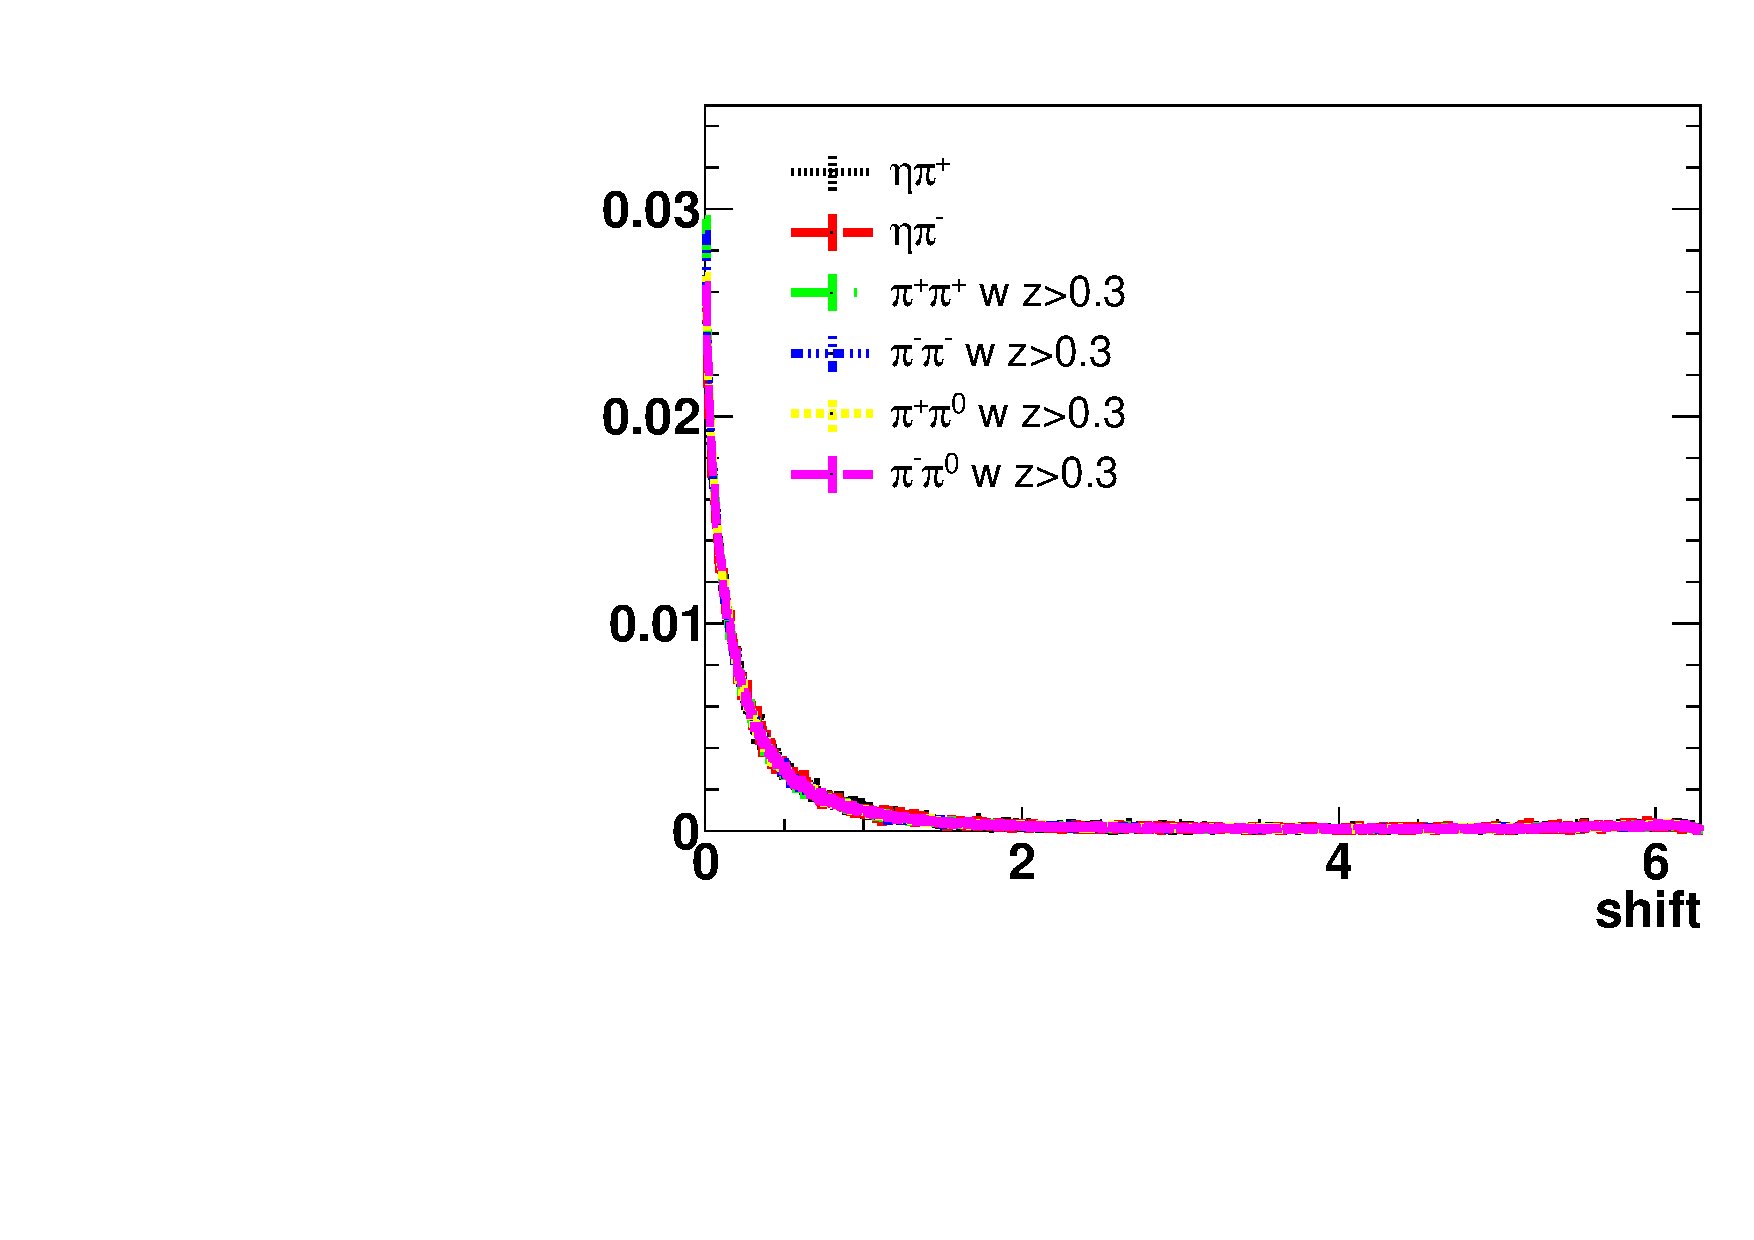
\includegraphics[width=60mm,natwidth=600,natheight=400]{figure_asy/corrections/etapairs_shift_compare_ComZ_8.pdf}}
  \caption{The resolution compare of all pion pairs.}
  \label{fig:shiftcompare}
\end{figure}
\iffalse
\begin{figure}[H]
  \centering     
  \subfigure[resolution of $(z_1,z_2)$ bins 8, $\pi^0\pi^+$ pairs]{\label{fig:shiftlastbin1}\includegraphics[width=60mm,natwidth=600,natheight=400]{figure_asy/corrections/Phi12pipiP0CombineZbin8_shift_fit.pdf}}
  \subfigure[resolution of $(z_1,z_2)$ bins 9, $\pi^0\pi^+$ pairs]{\label{fig:shiftlastbin2}\includegraphics[width=60mm,natwidth=600,natheight=400]{figure_asy/corrections/Phi12pipiP0CombineZbin9_shift_fit.pdf}}
  \caption{The resolution of $\pi^0\pi^+$ after adding $\pi^0\pi^-$.}
  \label{fig:shiftlastbin}
\end{figure}
\fi

Real Collins angle ($\phi_{12}^{\text{real}}$) can be simulated by drawing random numbers from a cosine-modulated distribution with range $[-\pi,\pi]$. To add $10\%$ inject asymmetry on the numerators of double ratio, $1+0.1*cos(x)$ is used to be the distribution function of $\pi^0\pi^+$ and $\pi^0\pi^-$. Uniform random numbers from $[-\pi,\pi]$ is generated to be the Collins angle of like sign charged pion pairs. Now the double ratio asymmetry should be a cosine module distribution with amplitude $0.1$. To better simulate the smearing effect occurs in experiment, the injections are chosen in the way that after applying smearing effect we can generate similar output with experimental data.

To simulate the smearing effect, a random Collins angle shift is drawn from the corresponding resolution function. By adding $\pm\Delta\phi_{12}$ to real Collins angle $\phi_{12}^{\text{real}}$ we obtain the smeared Collins angle $\phi_{12}^{\text{measure}}$. 

Besides Collins angles, the $P_t$ value of hadron pairs is also changed and this may leads to $P_t$ bin transfer when the inaccurate $P_t$ falls in a different $P_t$ bin. In order to simulate this $P_t$ bin conversion, we create a transmission matrix for each hadron pair type by comparing the yield of the original real bins and the smeared measured bins. %The eventsremain in the original $P_t$ bin as well as the ones changed to other bins when thrust axis is altered. 
For example, the $P_t$ transmission matrix for $\pi^0\pi^-$ is,
\begin{table}[H]\footnotesize
\centering
\begin{tabular}{|@{}l|c|c|c|c|}
\hline
 \diagbox[width=8em,trim=l]{Measured bin}{Real bin}&  0 & 1 & 2 & 3 \\ \hline
0	&	0.765	&	0.214	&	0.018	&	0.003 \\ \hline
1	&	0.133	&	0.717	&	0.140	&	0.010 \\ \hline
2	&	0.016	&	0.181	&	0.689	&	0.113 \\ \hline
3	&	0.007	&	0.030	&	0.240	&	0.723 \\ \hline
\end{tabular}
\caption{$P_t$ transmission matrix for $\pi^0\pi^-$. Real bin is obtained using stable thrust axis and the measured bin is obtained from original thrust axis.}
\label{tab:pibinshift_example}
\end{table}
This matrix indicates that around $70\%$ events stay in the original $P_t$ bin while other events are changed to other bins. When a new event is generated, according to the transfer possibilities in the corresponding matrix, this event may be saved to a different $P_t$ bin. This event carries the Collins and smearing effect of the original bin but are mistakenly classified to a new $P_t$ bin. Instead of simulating the same amount of events for all bins, we generate the number of events that are proportional to the real yield of each bin. 

By adding the shift which is retrieved from the resolution distribution to the real Collins angle and assigning $P_t$ bin transfer, we completely simulated the smearing effect. 

As mentioned before, the injected asymmetry for each bin is unique and is designed to be close to real experimental asymmetry, namely the before smearing asymmetry. Hence after adding the smearing effect, the outcome would be similar with the experimental measured asymmetry.  Here we use one set of injection which outputs the asymmetries around the lower boundary of measured values, and another set to generate asymmetries that cover the higher boundary. The smearing correction factors obtained from those two sets are used to get the mean and uncertainty for this correction. Figure.~\ref{fig:simulatesmear} shows the distribution of simulated and measured Collins angle. It can be seen that the amplitude of our simulation reproduce the lower limit of measured asymmetry .
\begin{figure}[H]
 \centering     
  \subfigure[Simulated $z_1$ bins 2 with smearing effect]{\label{fig:simulatesmear1}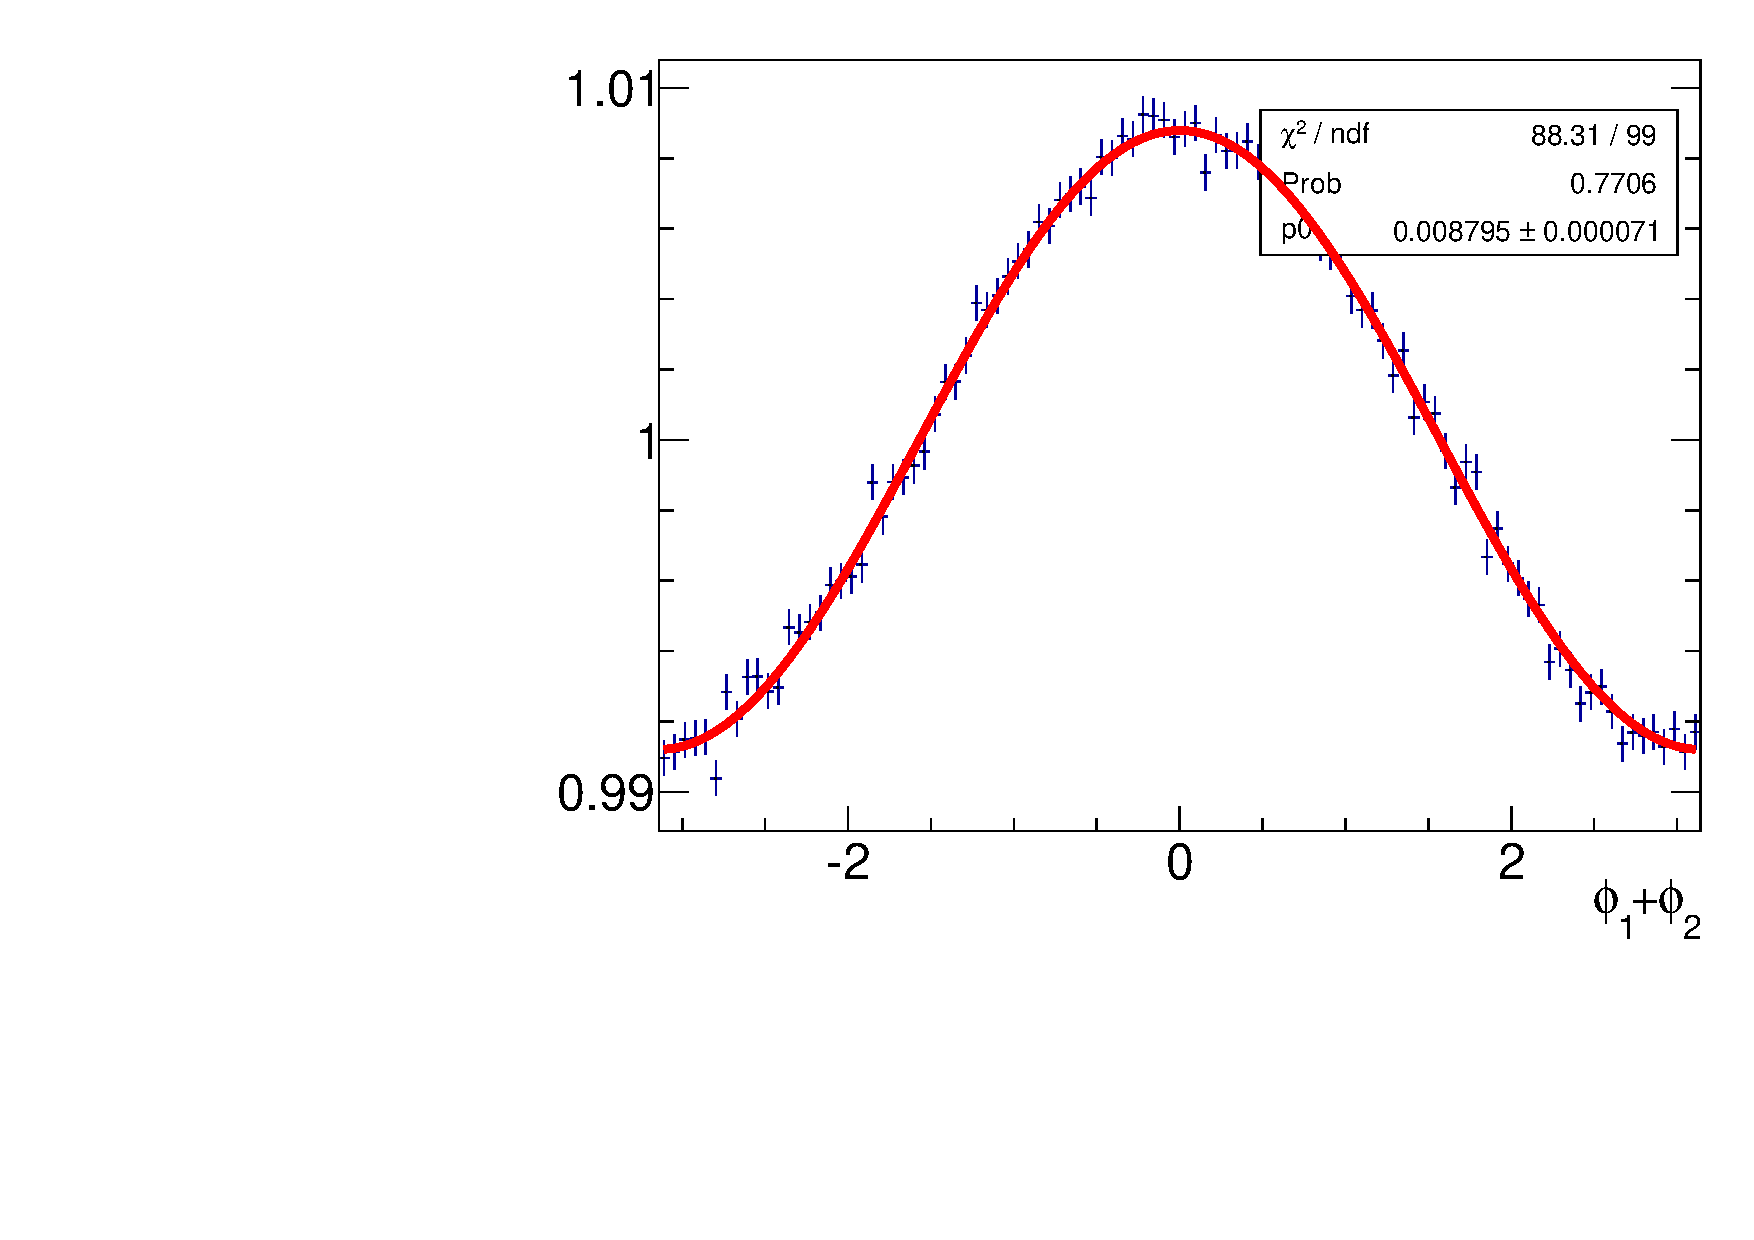
\includegraphics[width=60mm,natwidth=600,natheight=400]{figure_asy/corrections/SinZ_2_1_3_ratio.pdf}}
  \subfigure[Experiment result of $z_1$ bins 2]{\label{fig:simulatesmear2}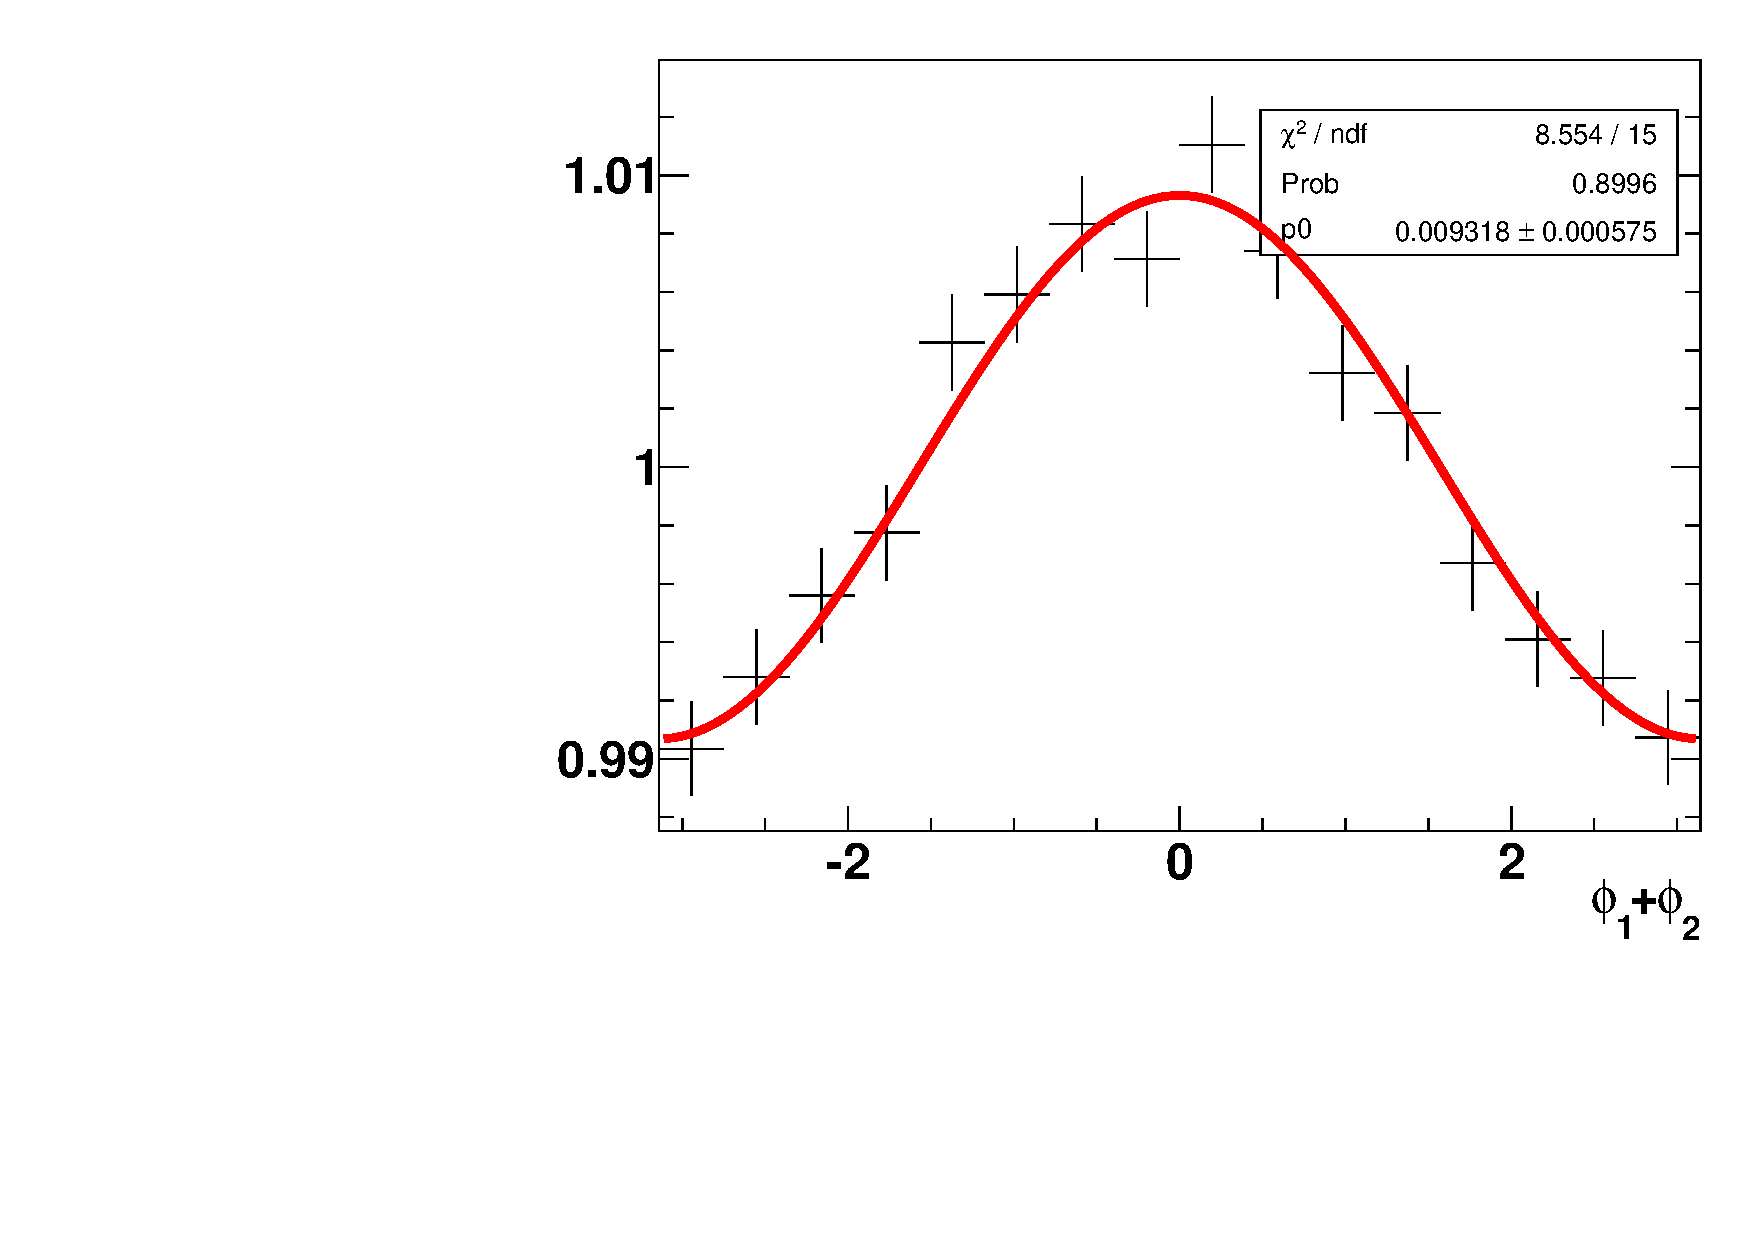
\includegraphics[width=60mm,natwidth=600,natheight=400]{figure_asy/corrections/SinZ2_1_3_2_4_ratio.pdf}}
  \caption[Simulated Collins angles and experiment Collins angles]{Simulated Collins angles and experiment Collins angles. Fig.~\ref{fig:simulatesmear1} shows simulated one and Fig.~\ref{fig:simulatesmear1} shows experimental data. }
  \label{fig:simulatesmear}
\end{figure}

The uncertainty comes from statistics can be neglected in this method, however using a constant injection for every bin cannot describe the smearing effect precisely. A constant injection implies that all events in the same bin contribute the same weight to the smearing effect, however the events that are close to thrust axis usually smeared most. Moreover, those events generally belong to low $P_t$ range and carry small Collins effect. By assigning the same weight to all events, we may overvalue those events and wrongly estimate the smearing effect. Theoretically we can implement a $P_t$ dependent injection by dividing all $z$ bins into several $P_t$ bins. But with fine binning we are lacking of statistics to generate resolution distribution. 


The regenerated smearing correction factor results are shown in the following tables.% \textcolor{red} {Table content will be updated once all factors are gathered}.
\begin{table}[H]\footnotesize
\centering
\begin{tabular}{|l|l|l|l|l|l|l|l|l|l|l|l|l|l|l|l|l|l|}
\hline
$z_1$ bin & $\pi^0$ simulated & $\pi^0$ directly measure & $\eta$ simulated  & $\eta$ directly measure  \\ \hline
0	&	1.26	&	1.21	&		&		\\ \hline
1	&	1.22	&	1.23	&		&		\\ \hline
2	&	1.23	&	1.23	&	1.28	&	1.25	\\ \hline
3	&	1.23	&	1.27	&	1.25	&	1.27	\\ \hline
4	&	1.26	&	1.25	&	1.26	&	1.30	\\ \hline
5	&	1.26	&	1.28	&	1.28	&	1.26	\\ \hline
6	&	1.34	&	1.31	&	1.32	&	1.33	\\ \hline
\end{tabular}
\caption{Thrust correction factors for $\pi^0$ and $\eta$ $z_1$ bins.}
\label{tab:sinzthrustfactor_compare}
\end{table}
It can be seen that those two methods agree for the bins without statistic problem. The estimation of $\eta$ using directly measured method~\ref{sec:etathrustcorrection} also give reasonable values. However, directly measured smearing has higher uncertainty due to the lacking of data while the statistic uncertainty in regenerated method can be negligible. So the simulated smearing correction factors will be used for final asymmetries. 
\begin{table}[H]\footnotesize
\centering
\begin{tabular}{|l|l|l|l|l|l|l|l|l|l|l|l|l|l|l|l|l|l|}
\hline
combined $z$ & $\pi^0$ simulated & $\pi^0$ directly measure & $\eta$ simulated  & $\eta$ directly measure  \\ \hline
0	&	1.19	&	1.22	&		&		\\ \hline
1	&	1.25	&	1.22	&		&		\\ \hline
2	&	1.26	&	1.29	&		&		\\ \hline
3	&	1.35	&	1.35	&		&		\\ \hline
4	&	1.23	&	1.23	&	1.25	&	1.26	\\ \hline
5	&	1.27	&	1.23	&	1.27	&	1.30	\\ \hline
6	&	1.31	&	1.28	&	1.34	&	1.32	\\ \hline
7	&	1.26	&	1.22	&	1.27	&	1.22	\\ \hline
8	& 	1.27	&	1.24	&	1.30	&	1.29	\\ \hline
9	&	1.28	&	1.24	&	1.27	&	1.23	\\ \hline
\end{tabular}
\caption{Thrust correction factors for $\pi^0$ and $\eta$ $(z_1,z_2)$ bins.}
\label{tab:comzthrustfactor_compare}
\end{table}
The red numbers and $\eta$ directly measured corrections in Tab.~\ref{tab:comzthrustfactor} are estimated instead of measured, see section~\ref{sec:ThrustCorrectionFactors_pi0}.
\begin{table}[H]\footnotesize
\centering
\begin{tabular}{|l|l|l|l|l|l|l|l|l|l|l|l|l|l|l|l|l|l|}
\hline
$P_{t1}$ bin & $\pi^0$ simulated & $\pi^0$ directly measure & $\eta$ simulated  & $\eta$ directly measure  \\ \hline
0	&	1.41	&	1.38	&	1.68	&	1.68	\\ \hline
1	&	1.33	&	1.16	&	1.44	&	1.25	\\ \hline
2	&	1.24	&	1.13	&	1.27	&	1.16	\\ \hline
3	&	1.23	&	1.13	&	1.25	&	1.16	\\ \hline
\end{tabular}
\caption{Thrust correction factors for $\pi^0$ and $\eta$ $P_{t1}$ bins.}
\label{tab:sinptthrustfactor_compare}
\end{table}

\begin{table}[H]\footnotesize
\centering
\begin{tabular}{|l|l|l|l|l|l|l|l|l|l|l|l|l|l|l|l|l|l|}
\hline
combined $P_t$ & $\pi^0$ simulated & $\pi^0$ directly measure & $\eta$   simulated  & $\eta$  directly measure  \\ \hline
0	&	0.59	&	1.57	&	2.17	&	2.17	\\ \hline
1	&	1.92	&	1.36	&	1.34	&	1.67	\\ \hline
2	&	1.41	&	1.27	&	1.91	&	1.66	\\ \hline
3	&	1.38	&	1.27	&	1.70	&	1.62	\\ \hline
4	&	1.39	&	1.18	&	1.80	&	1.23	\\ \hline
5	&	1.36	&	1.13	&	1.69	&	1.19	\\ \hline
6	&	1.32	&	1.11	&	1.54	&	1.19	\\ \hline
7	&	1.19	&	1.11	&	1.24	&	1.12	\\ \hline
8	&	1.25	&	1.08	&	1.35	&	1.09	\\ \hline
9	&	1.17	&	1.07	&	1.22	&	1.07	\\ \hline
\end{tabular}
\caption{Thrust correction factors for $\pi^0$ and $\eta$ $(P_{t1},P_{t2})$ bins.}
\label{tab:comptthrustfactor_compare}
\end{table}
\fi

%%%%%%%%%

\subsection{Results After Corrections}

Figures~\ref{fig:pi0result} and~\ref{fig:etaresult} display the asymmetry after background and thrust-smearing corrections. Notice that the plots have different scales. 
Also, {\bf a bug was discovered in the background correction that still affects these plots} (but not the final result plots). The effect is that the uncertainties of the background correction are inflated.
\begin{figure}[t]
  \centering     \tiny
  \subfigure[$z_1$ bins]{\label{fig:pi0result1}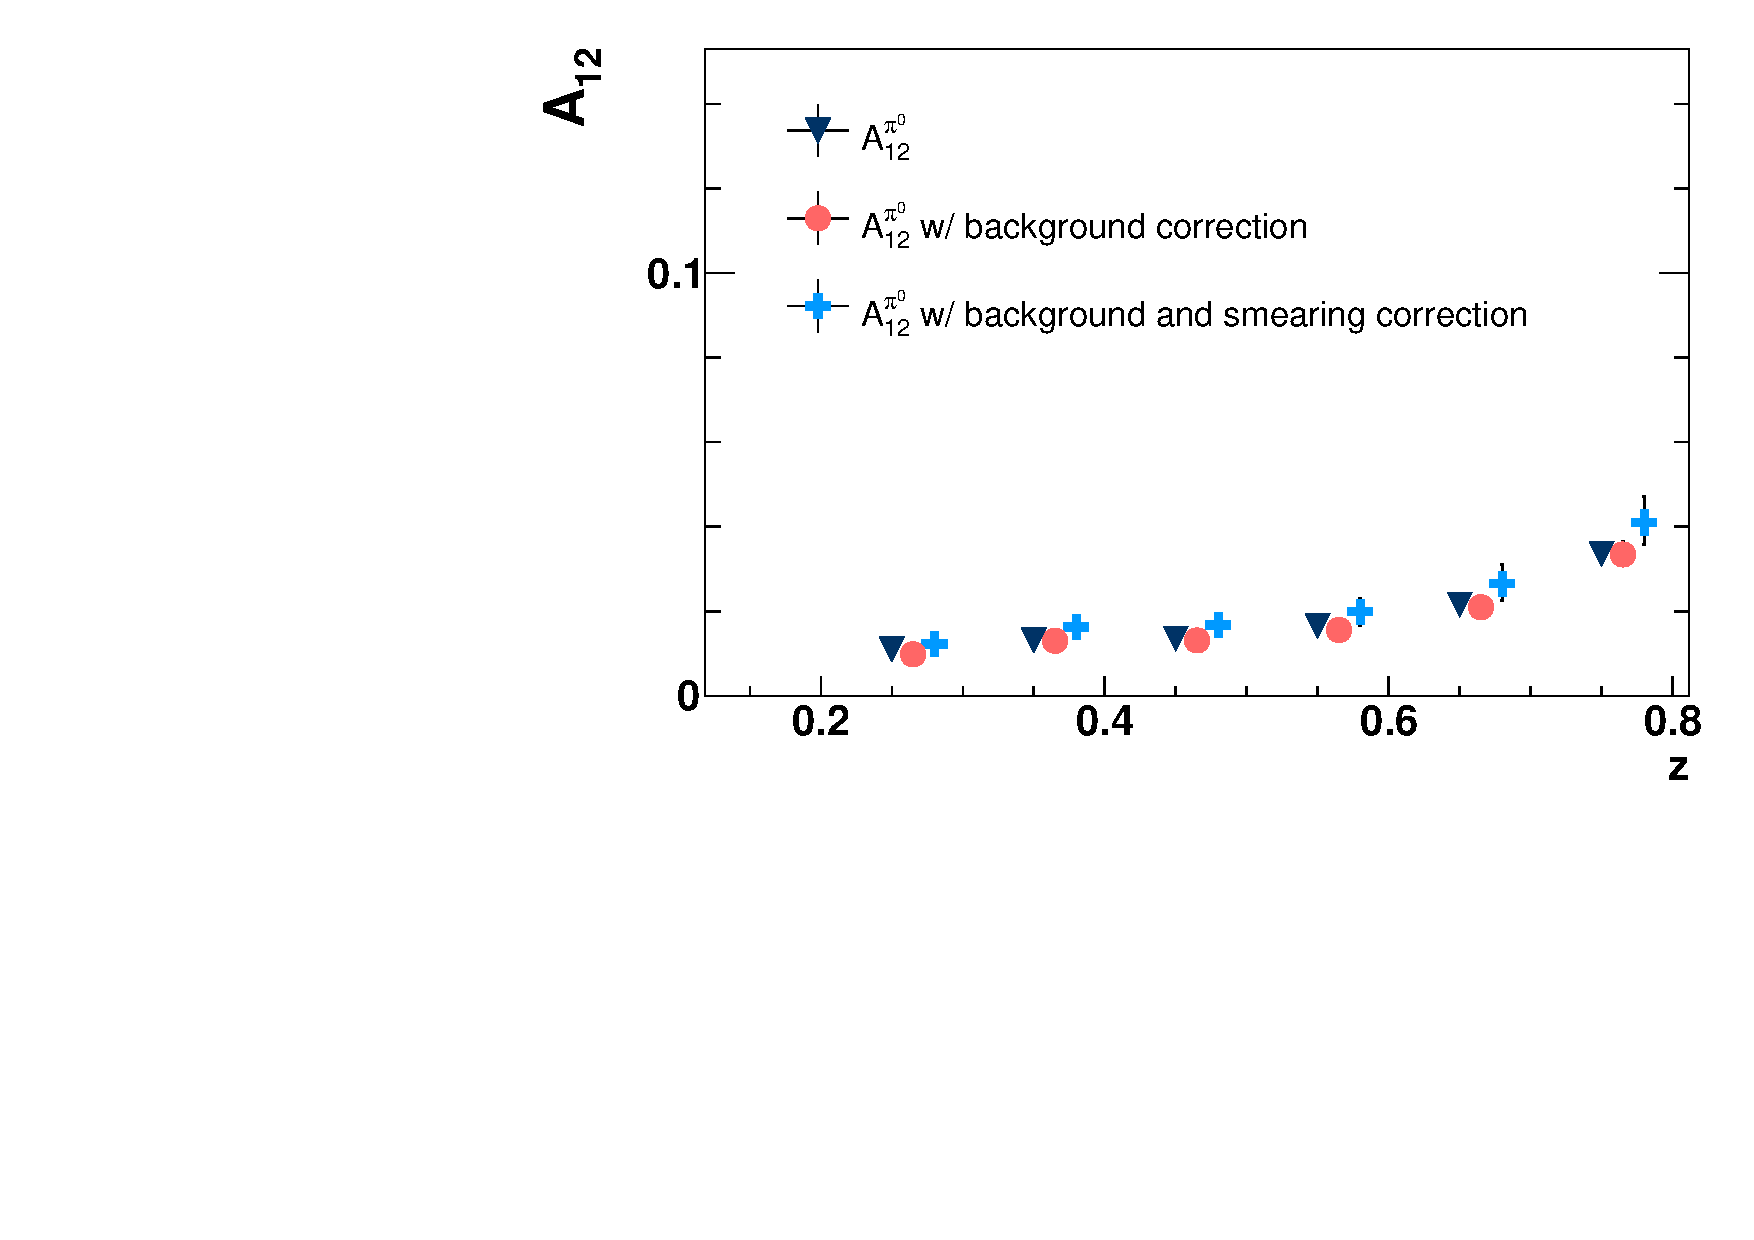
\includegraphics[width=60mm,natwidth=600,natheight=400]{figure_asy/Pi0AllCorrection0.pdf}}
  \subfigure[$P_{t1}$ bins]{\label{fig:pi0result3}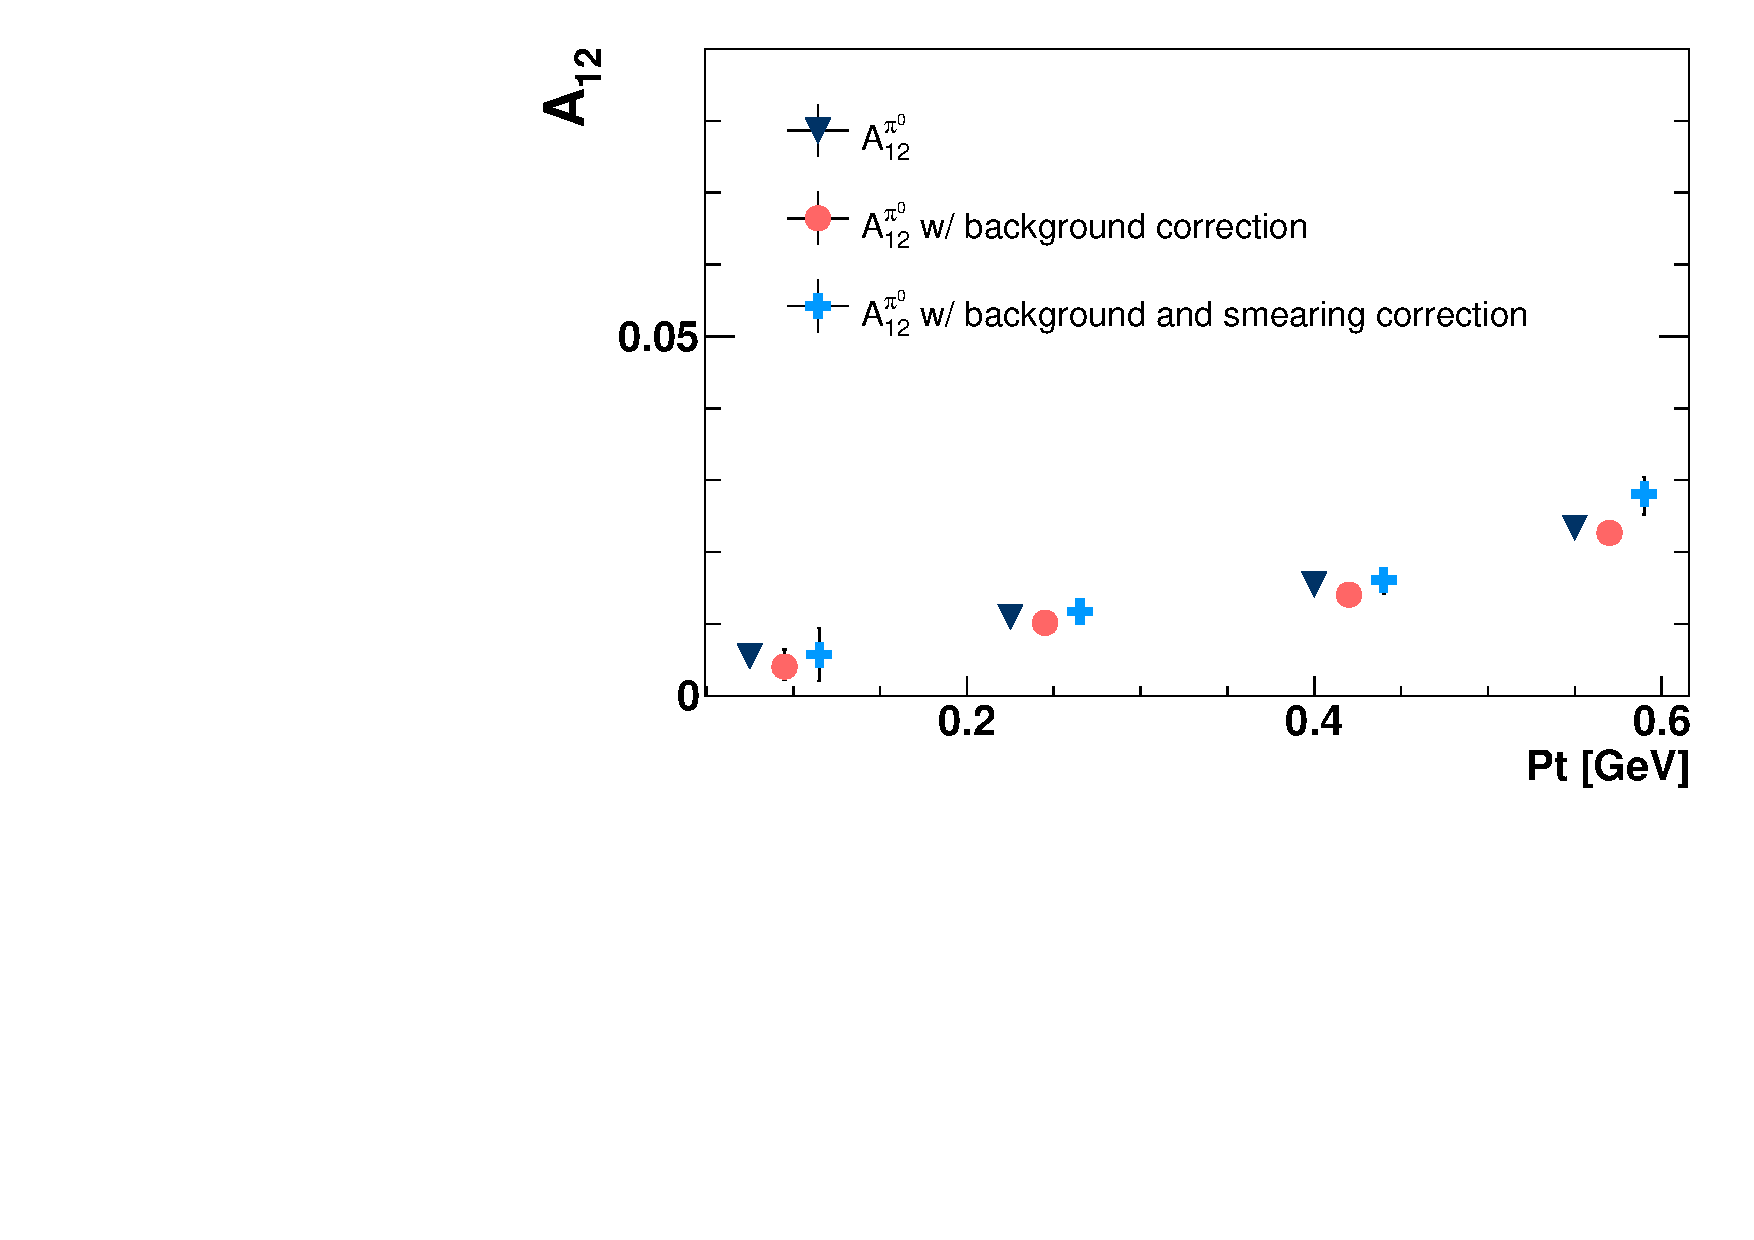
\includegraphics[width=60mm,natwidth=600,natheight=400]{figure_asy/Pi0AllCorrection2.pdf}}
  \subfigure[$(z_1,z_2)$ bins]{\label{fig:pi0result2}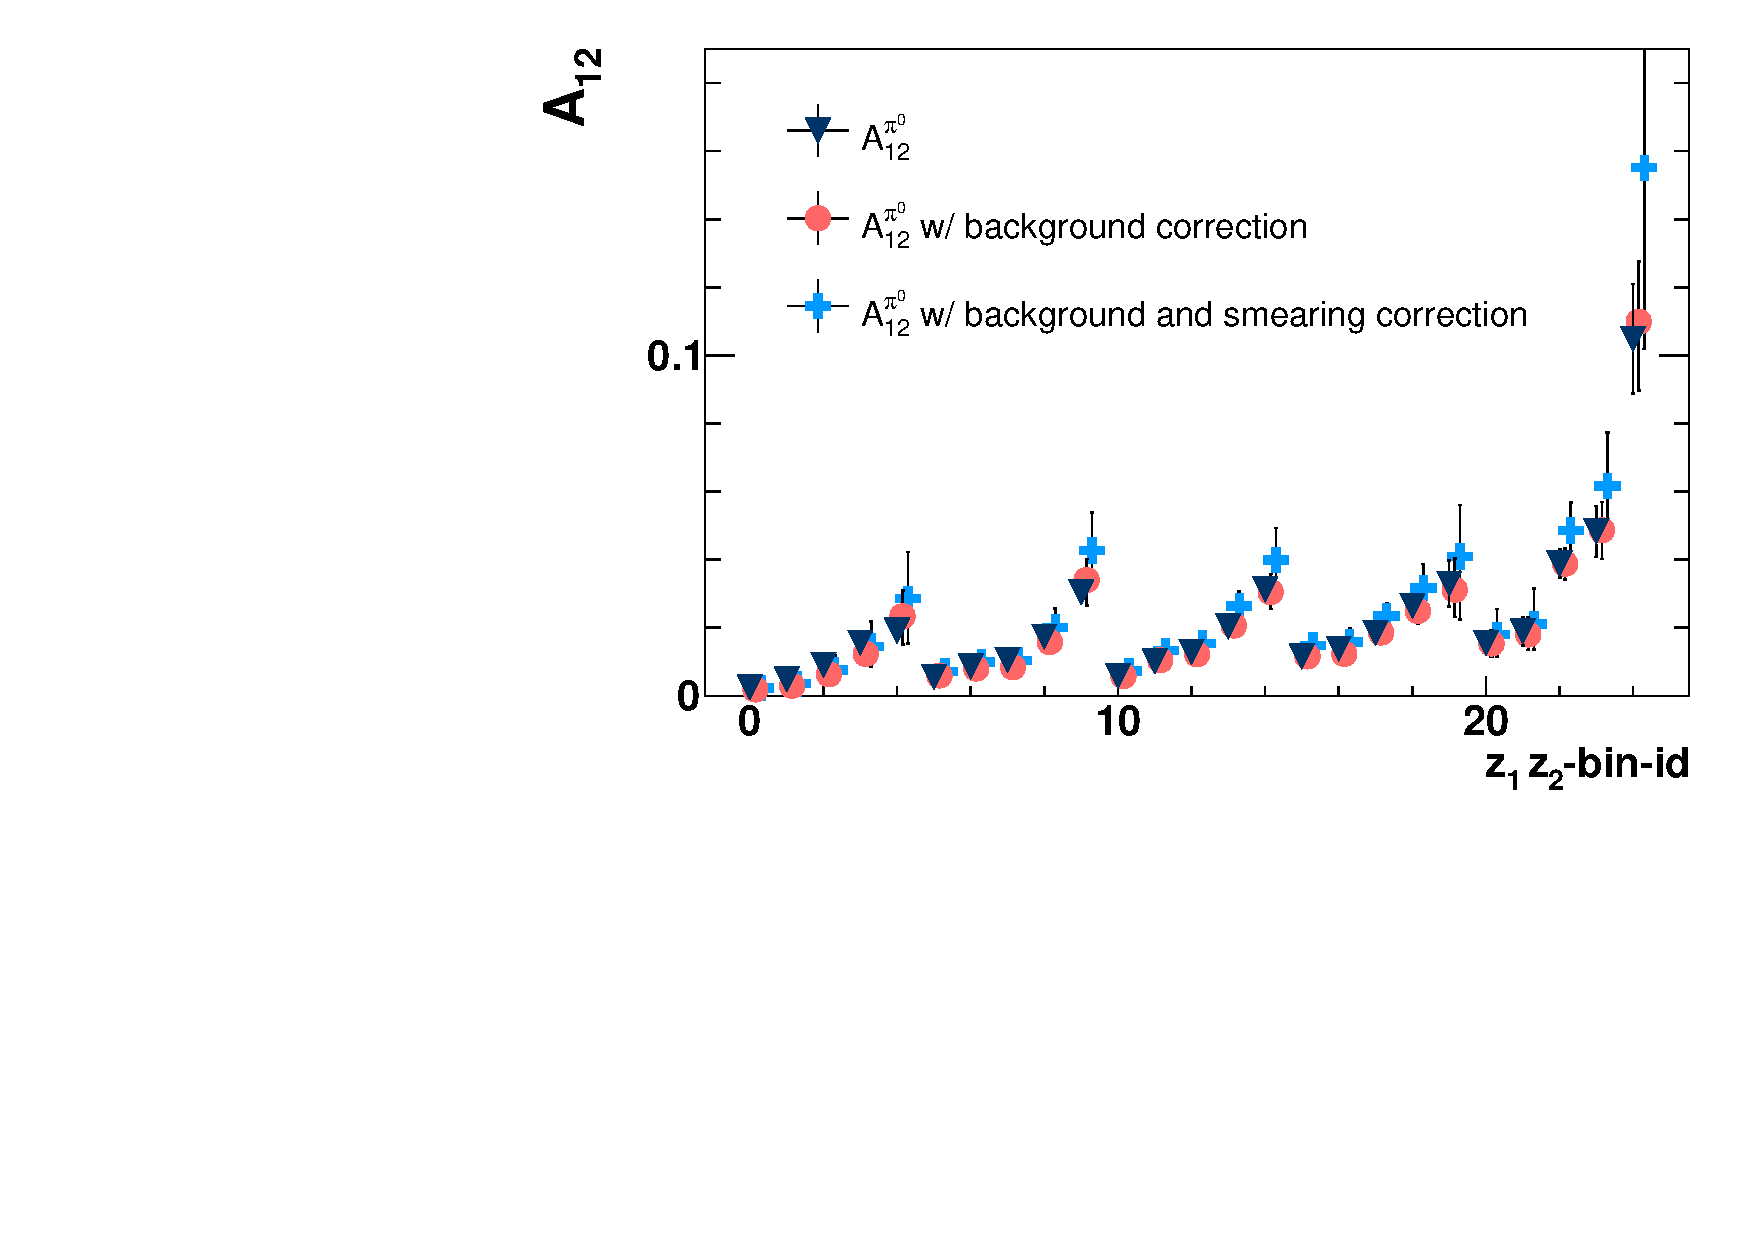
\includegraphics[width=60mm,natwidth=600,natheight=400]{figure_asy/Pi0AllCorrection1.pdf}}
  \subfigure[$(P_{t1},P_{t2})$ bins]{\label{fig:pi0result4}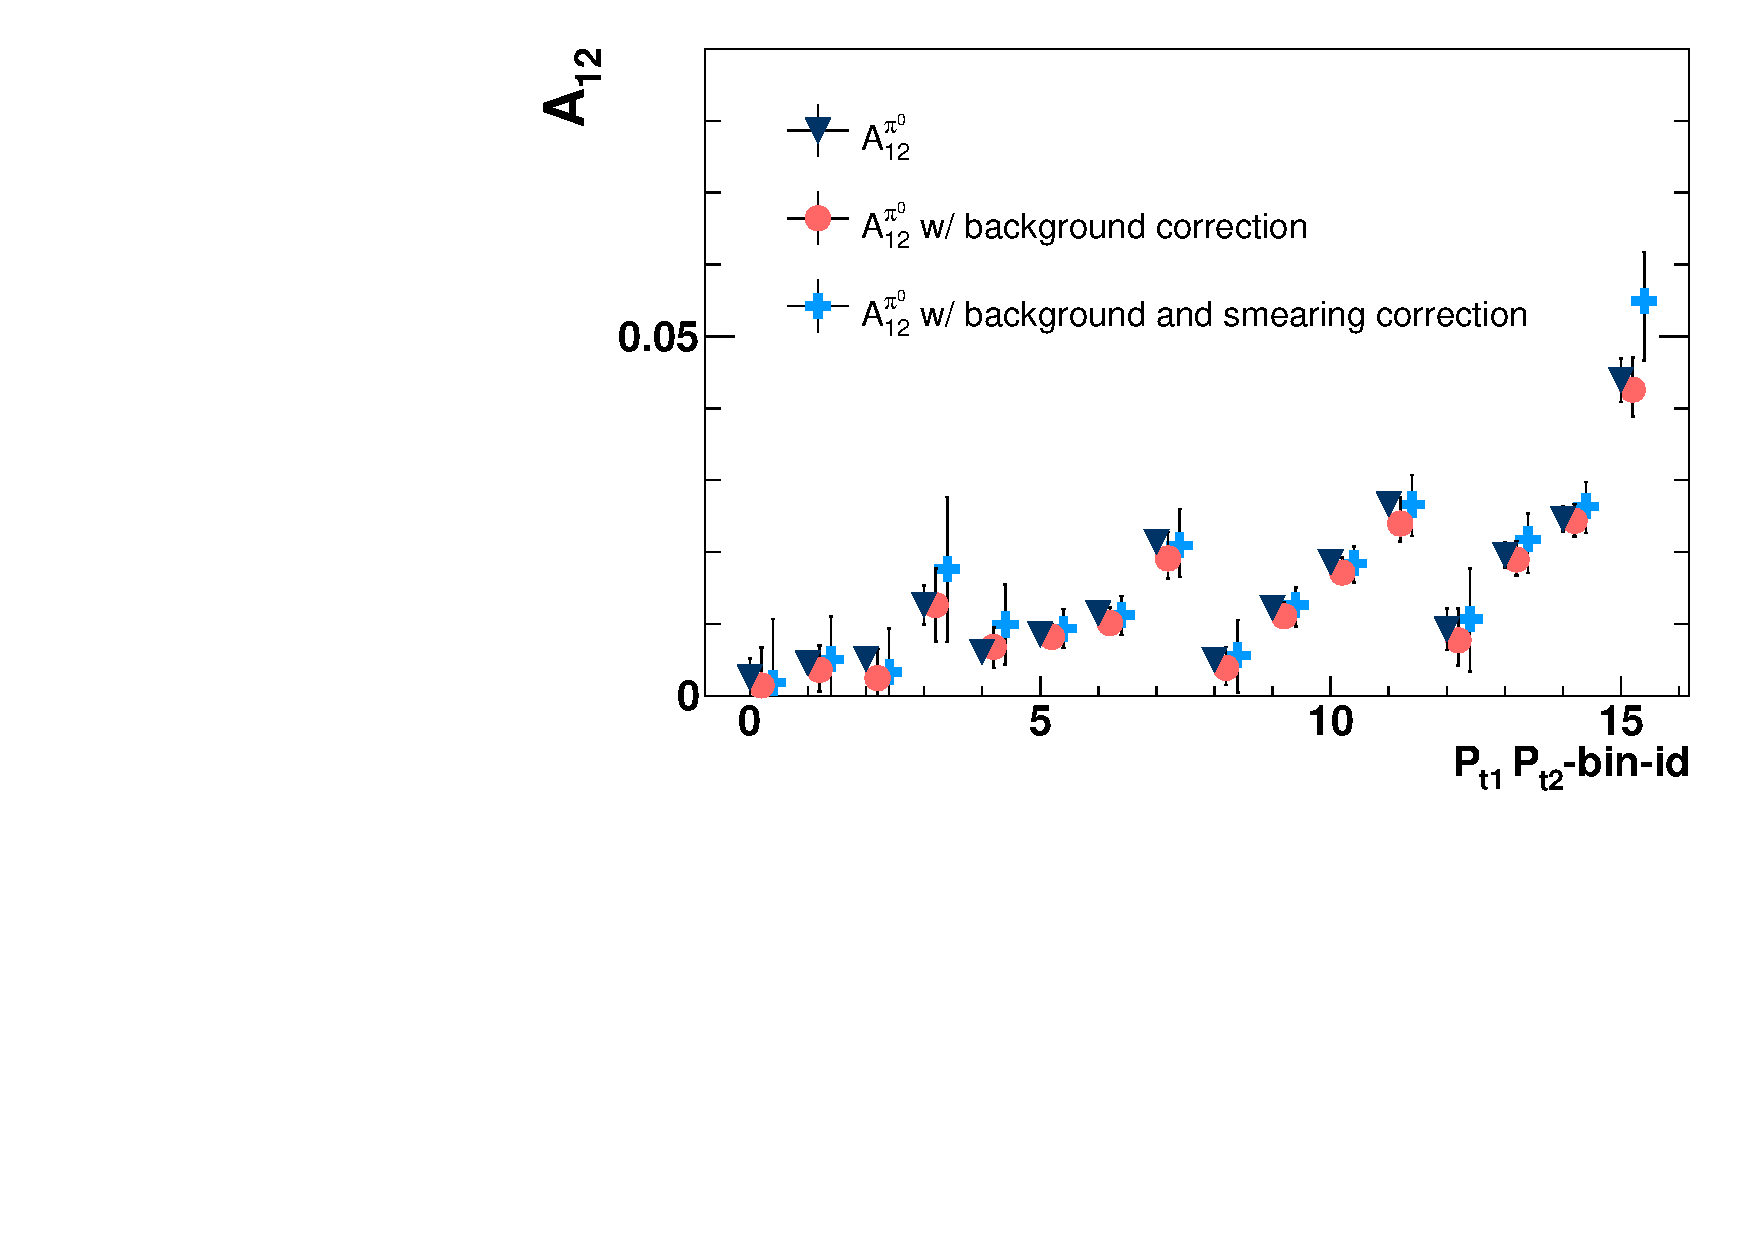
\includegraphics[width=60mm,natwidth=600,natheight=400]{figure_asy/Pi0AllCorrection3.pdf}}
  \caption[$\pi^0$ double ratio asymmetries $A^{\pi^0}_{12}$ after background and thrust-smearing corrections for different kinematic bins]{$\pi^0$ double ratio asymmetries $A^{\pi^0}_{12}$ for different kinematic bins. The triangle points are the originally measured asymmetry. Round points are asymmetries after background corrections. Cross points are asymmetries after background and thrust smearing correction, and the uncertainties include background and smearing corrections. {\bf Note that the results in these plots use an incorrect background subtraction, see text for details}}
  \label{fig:pi0result}
\end{figure}

\begin{figure}[h]
  \centering     \tiny
  \subfigure[$z_1$ bins]{\label{fig:etaresult1}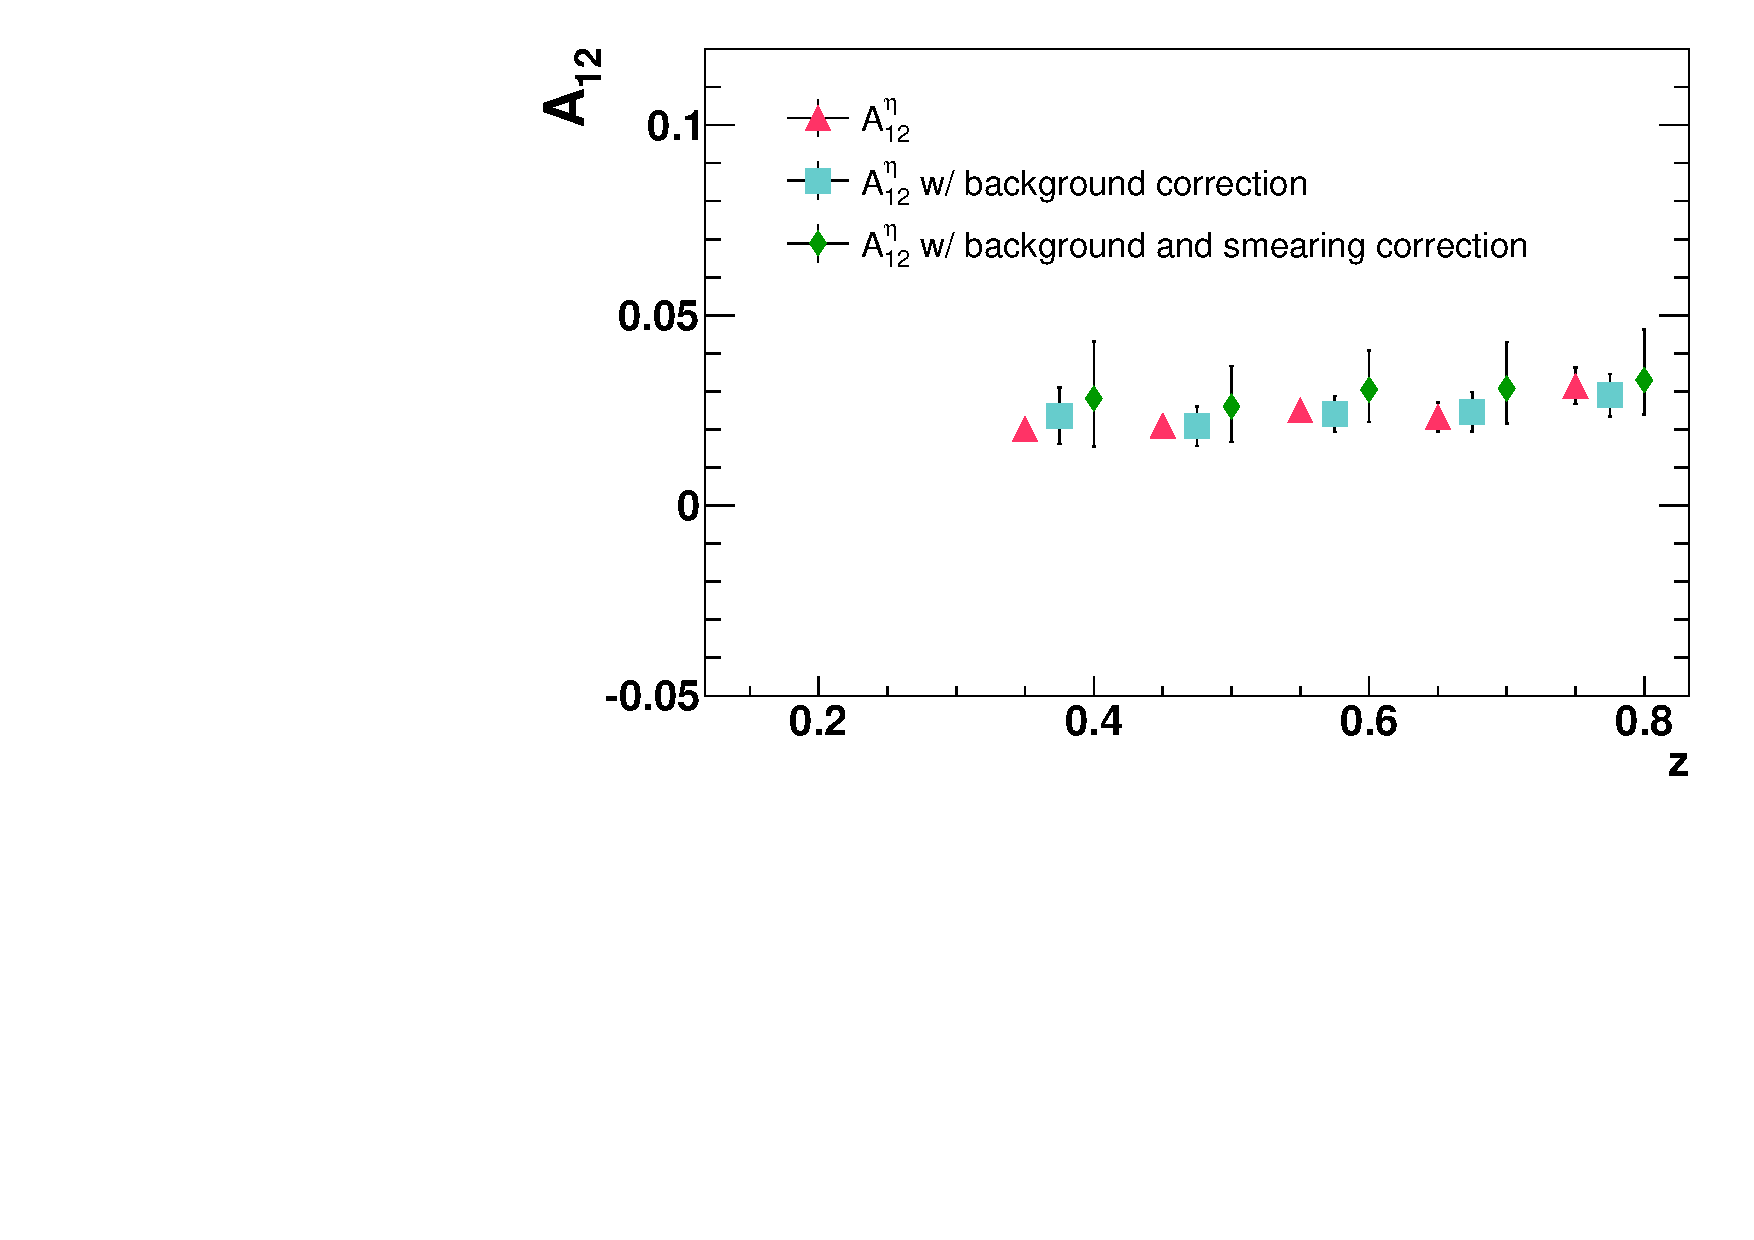
\includegraphics[width=60mm,natwidth=600,natheight=400]{figure_asy/EtaAllCorrection0.pdf}}
  \subfigure[$P_{t1}$ bins]{\label{fig:etaresult3}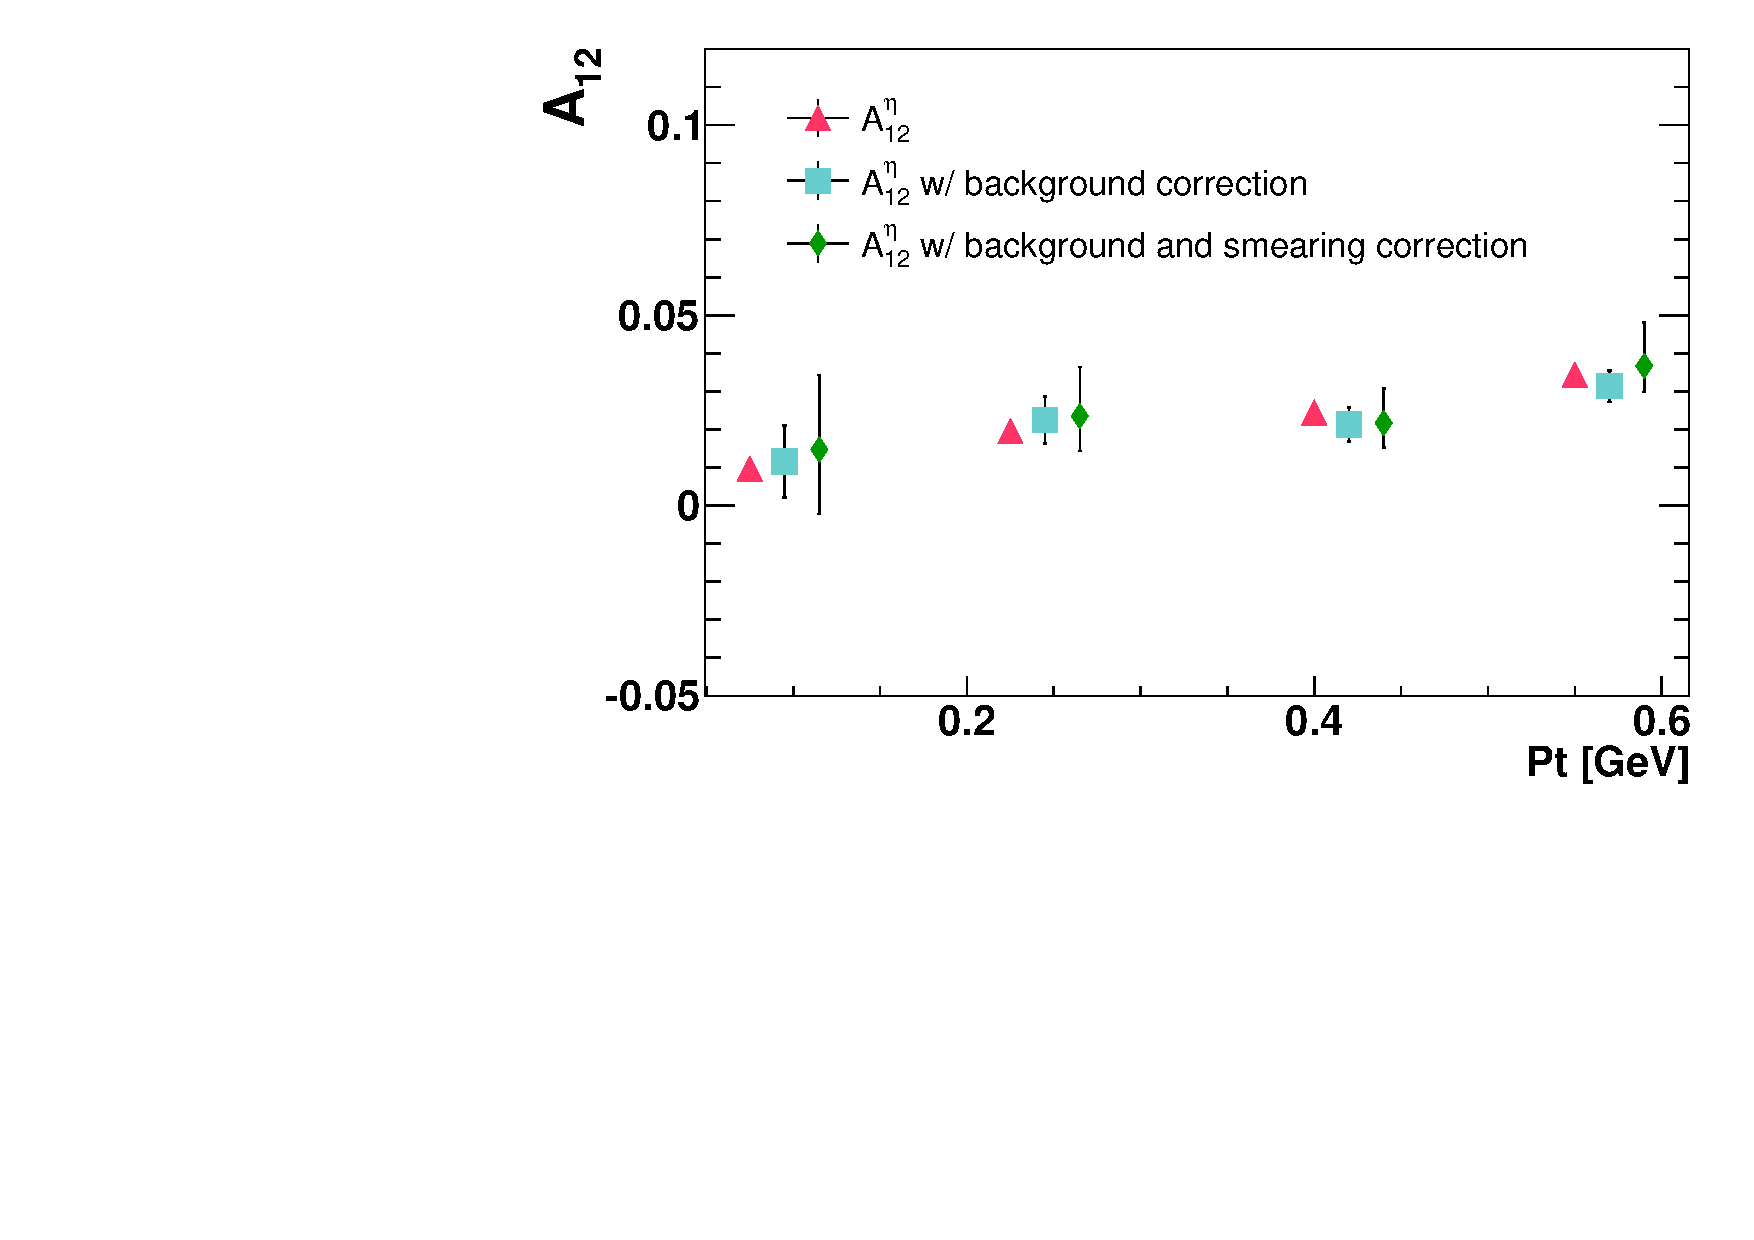
\includegraphics[width=60mm,natwidth=600,natheight=400]{figure_asy/EtaAllCorrection2.pdf}}
  \subfigure[$(z_1,z_2)$ bins]{\label{fig:etaresult2}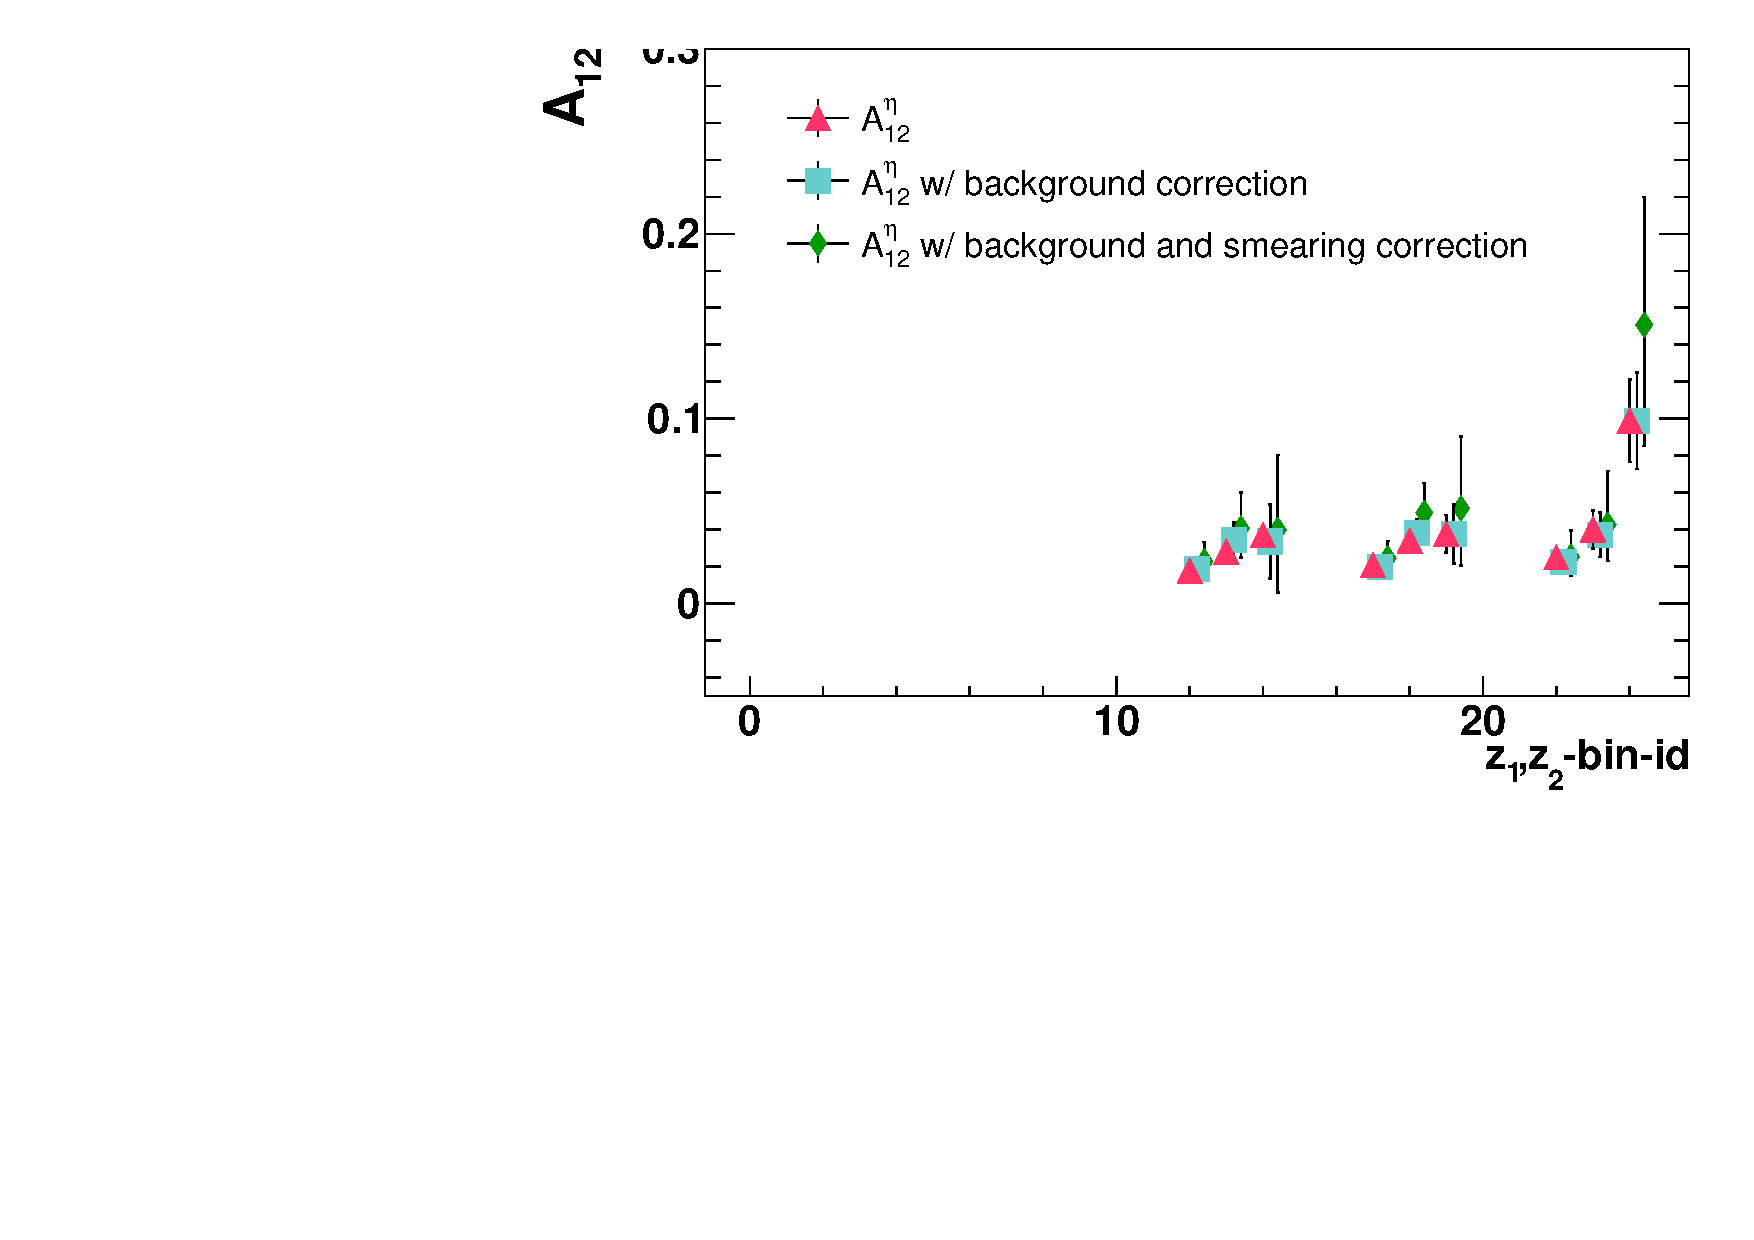
\includegraphics[width=60mm,natwidth=600,natheight=400]{figure_asy/EtaAllCorrection1.pdf}}
  \subfigure[$(P_{t1},P_{t2})$ bins]{\label{fig:etaresult4}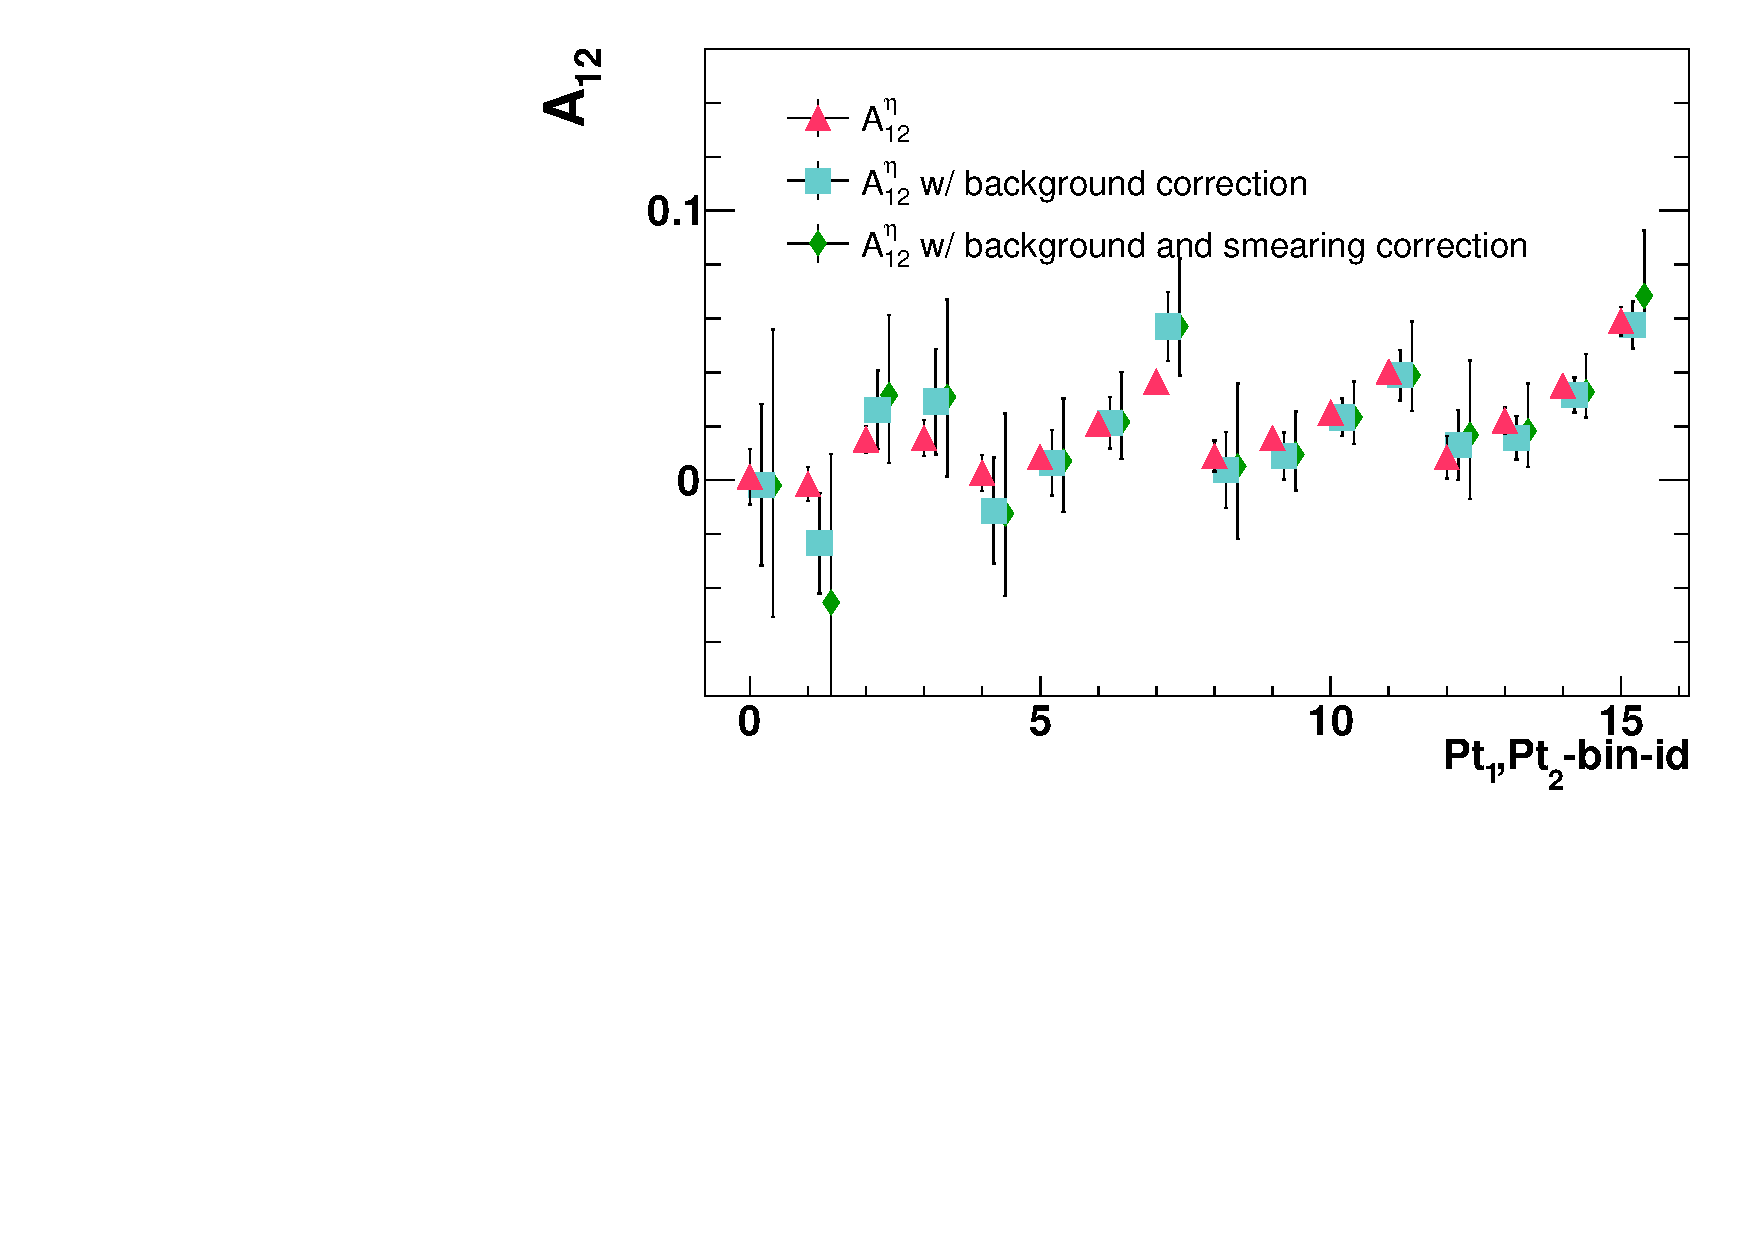
\includegraphics[width=60mm,natwidth=600,natheight=400]{figure_asy/EtaAllCorrection3.pdf}}
  \caption[$\eta$ double ratio asymmetries $A^{\eta}_{12}$ after background and thrust-smearing corrections for different kinematic bins]{$\eta$ double ratio asymmetries $A^{\eta}_{12}$ for different kinematic bins. The triangle points are the originally measured asymmetry. Square points are asymmetries after background corrections. Diamond points are asymmetries after background and thrust smearing correction. The uncertainties include the systematics from background and smearing correction. {\bf Note that the results in these plots use an incorrect background subtraction, see text for details}}
  \label{fig:etaresult}
\end{figure}


\subsection{Charm Contribution}
\label{sec:charmcontribution}
The contribution of charm fragmentation to the charged-pion Collins asymmetry was studied in Ref.~\cite{ChargedPionResult2}. 
In this section, the proportion of charm for each kinematic bin is estimated by using the standard Belle MC. The yield of each hadron pair in MC \(uds\) and MC charm has been determined for each bin, in particular, the ratio $\nicefrac{\mathrm{charm}}{\mathrm{uds}}$ is determined for each bin using the same cuts as in the analysis. Results show that the percentage of charm contributions are close, within 2\%, with the exception of the first $z$ bin where asymmetries are small, in all charged and neutral pion pairs and their mean value is used for the charm ratio. The charm percentage contribution in each bin is listed in Tables~\ref{tab:sinzcharmratio}--\ref{tab:comptcharmratio}. {\bf No correction} is made because the extraction of the charm signal from $D^0$s would not be precise. Once further studies of the Collins effect for charm have become available, for example from Belle II, the following ratios will in principle allow corrections in global fits, however, we acknowledge that for the optimal correction matching the respective phase spaces will be challenging.

We note that in general the charm fractions of pairs including $\eta$ mesons tend to be somewhat higher than the fractions involving only pions. This effect is more pronounced at larger $z$ and large $P_t$. For most bins the difference is not more than 5\%. If we assume that particles from charm decay carry a much smaller asymmetry, since they come from a decay chain involving the weak decay of a $D$ meson, this would lead, to first order, to a suppression of the $\eta$ asymmetries with respect to the pion asymmetries by the same percentage.


\begin{table}[H]\footnotesize
\centering
\begin{tabular}{|c||c|c|c|c|c|c|}
\hline
$z_1$ & $\pi^{\pm}\pi^{\pm}$ & $\pi^{\pm}\pi^0$ & $\eta\pi^{\pm}$ & $\pi^0\pi^{\pm}$ $(z>0.3)$ & $\pi^{\pm}\pi^{\pm}$ $(z>0.3)$ \\ \hline\hline
%[0.1,0.2]       &	30.59	&	39.08	&		&		&			\\ \hline
[0.2,0.3]	&	22.24	&	23.90	&		&		&		\\ \hline
[0.3,0.4]	&	18.34	&	18.64	&	19.71	&	15.98	&	15.74	\\ \hline
[0.4,0.5]	&	16.48	&	16.17	&	16.85	&	13.73	&	13.72	\\ \hline
[0.5,0.6]	&	14.50	&	13.53	&	15.63	&	11.33	&	11.86	\\ \hline
[0.6,0.7]	&	10.12	&	8.85	&	13.04	&	7.20	&	8.30	\\ \hline
[0.7,1.0]	&	4.66	&	3.63	&	7.18	&	2.90	&	4.08	\\ \hline\end{tabular}
\caption[Charm ratio in $z_1$ bins]{Charm ratio in $z_1$ bins. All numbers are in percent.}
\label{tab:sinzcharmratio}
\end{table}

\begin{table}[H]\footnotesize
\centering
\begin{tabular}{|c|c||c|c|c|c|c|c|}
\hline
 $z_1$& $z_2$ & $\pi^{\pm}\pi^{\pm}$ & $\pi^{\pm}\pi^0$ & $\eta\pi^{\pm}$ & $\pi^0\pi^{\pm}$ $(z>0.3)$ & $\pi^{\pm}\pi^{\pm}$ $(z>0.3)$ \\ \hline\hline
[0.1,0.2]	&	[0.1,0.2]	&	36.75	&	41.87	&		&		&		\\ \hline
[0.1,0.2]	&	[0.2,0.3]	&	30.63	&	35.32	&		&		&		\\ \hline
[0.1,0.2]	&	[0.3,0.5]	&	24.97	&	28.98	&		&		&		\\ \hline
[0.1,0.2]	&	[0.5,0.7]	&	18.98	&	22.47	&		&		&		\\ \hline
[0.1,0.2]	&	[0.7,1.0]	&	6.45	&	7.80	&		&		&		\\ \hline \hline
[0.2,0.3]	&	[0.1,0.2]	&	30.65	&	32.92	&		&		&		\\ \hline
[0.2,0.3]	&	[0.2,0.3]	&	25.52	&	27.40	&		&		&		\\ \hline
[0.2,0.3]	&	[0.3,0.5]	&	20.55	&	22.11	&		&		&		\\ \hline
[0.2,0.3]	&	[0.5,0.7]	&	15.75	&	16.82	&		&		&		\\ \hline
[0.2,0.3]	&	[0.7,1.0]	&	5.44	&	5.76	&		&		&		\\ \hline\hline
[0.3,0.5]	&	[0.1,0.2]	&	25.13	&	25.47	&		&		&		\\ \hline
[0.3,0.5]	&	[0.2,0.3]	&	20.71	&	20.85	&		&		&		\\ \hline
[0.3,0.5]	&	[0.3,0.5]	&	15.96	&	16.28	&	19.85	&	16.28	&	16.05	\\ \hline
[0.3,0.5]	&	[0.5,0.7]	&	11.70	&	12.01	&	14.66	&	12.01	&	11.69	\\ \hline
[0.3,0.5]	&	[0.7,1.0]	&	4.10	&	3.95	&	4.66	&	3.95	&	4.43	\\ \hline\hline
[0.5,0.7]	&	[0.1,0.2]	&	19.22	&	18.12	&		&		&		\\ \hline
[0.5,0.7]	&	[0.2,0.3]	&	15.92	&	14.90	&		&		&		\\ \hline
[0.5,0.7]	&	[0.3,0.5]	&	11.75	&	11.13	&	16.13	&	11.13	&	11.74	\\ \hline
[0.5,0.7]	&	[0.5,0.7]	&	8.03	&	7.74	&	11.02	&	7.74	&	7.78	\\ \hline
[0.5,0.7]	&	[0.7,1.0]	&	2.74	&	2.65	&	3.22	&	2.65	&	2.89	\\ \hline\hline
[0.7,1.0]	&	[0.1,0.2]	&	6.88	&	5.47	&		&		&		\\ \hline
[0.7,1.0]	&	[0.2,0.3]	&	5.72	&	4.59	&		&		&		\\ \hline
[0.7,1.0]	&	[0.3,0.5]	&	4.10	&	3.20	&	7.82	&	3.20	&	4.44	\\ \hline
[0.7,1.0]	&	[0.5,0.7]	&	2.77	&	1.91	&	5.11	&	1.91	&	2.91	\\ \hline
[0.7,1.0]	&	[0.7,1.0]	&	1.11	&	0.90	&	2.40	&	0.90	&	1.28	\\ \hline
\end{tabular}
\caption[Charm ratio in combined $z_{1}$--$z_{2}$ bins]{Charm ratio in combined $z_{1}$--$z_{2}$ bins. All numbers are in percent.}
\label{tab:comzcharmratio}
\end{table}

\begin{table}[H]\footnotesize
\centering
\begin{tabular}{|c||c|c|c|c|c|c|}
\hline
$P_{t1}$ [GeV]  &$\pi^{\pm}\pi^{\pm}$ & $\pi^{\pm}\pi^0$ & $\eta\pi^{\pm}$ & $\pi^0\pi^{\pm}$ $(z>0.3)$ & $\pi^{\pm}\pi^{\pm}$ $(z>0.3)$ \\ \hline\hline
[0,0.15]	&	19.74	&	21.44	&	15.67	&	13.32	&	12.91	\\ \hline
[0.15,0.30]	&	19.60	&	21.08	&	16.16	&	13.57	&	13.20	\\ \hline
[0.30,0.50]	&	18.76	&	19.40	&	18.19	&	14.60	&	14.38	\\ \hline
[0.50,3.0]	&	18.75	&	18.19	&	21.10	&	15.45	&	15.54	\\ \hline
\end{tabular}
\caption[Charm ratio in $P_{t1}$ bins]{Charm ratio in $P_{t1}$ bins. All numbers are in percent.}
\label{tab:sinptcharmratio}
\end{table}

\begin{table}[H]\footnotesize
\centering
\begin{tabular}{|c|c||c|c|c|c|c|c|}
\hline
$P_{t1}$ [GeV] & $P_{t2}$ [GeV] &$\pi^{\pm}\pi^{\pm}$ & $\pi^{\pm}\pi^0$ & $\eta\pi^{\pm}$ & $\pi^0\pi^{\pm}$ $(z>0.3)$ & $\pi^{\pm}\pi^{\pm}$ $(z>0.3)$ \\ \hline\hline
[0,0.15]	&	[0,0.15]	&	20.15	&	21.93	&	13.80	&	11.75	&	11.81	\\ \hline
[0,0.15]	&	[0.15,0.30]	&	20.07	&	21.82	&	14.74	&	12.32	&	12.01	\\ \hline
[0,0.15]	&	[0.30,0.50]	&	19.28	&	20.87	&	15.86	&	13.54	&	13.15	\\ \hline
[0,0.15]	&	[0.50,3.0]	&	19.44	&	21.33	&	17.92	&	15.43	&	14.58	\\ \hline\hline
[0.15,0.30]	&	[0,0.15]	&	20.10	&	21.55	&	14.37	&	12.09	&	12.05	\\ \hline
[0.15,0.30]	&	[0.15,0.30]	&	19.92	&	21.42	&	14.71	&	12.43	&	12.29	\\ \hline
[0.15,0.30]	&	[0.30,0.50]	&	19.12	&	20.59	&	16.72	&	13.87	&	13.52	\\ \hline
[0.15,0.30]	&	[0.50,3.0]	&	19.22	&	20.79	&	18.32	&	15.65	&	14.69	\\ \hline\hline
[0.30,0.50]	&	[0,0.15]	&	19.36	&	19.91	&	16.41	&	13.10	&	13.31	\\ \hline
[0.30,0.50]	&	[0.15,0.30]	&	19.15	&	19.79	&	16.78	&	13.48	&	13.51	\\ \hline
[0.30,0.50]	&	[0.30,0.50]	&	18.24	&	18.87	&	18.60	&	14.88	&	14.67	\\ \hline
[0.30,0.50]	&	[0.50,3.0]	&	18.09	&	18.97	&	20.64	&	16.70	&	15.84	\\ \hline\hline
[0.50,3.0]	&	[0,0.15]	&	19.55	&	18.84	&	18.79	&	14.10	&	14.69	\\ \hline
[0.50,3.0]	&	[0.15,0.30]	&	19.38	&	18.66	&	19.86	&	14.38	&	14.98	\\ \hline
[0.50,3.0]	&	[0.30,0.50]	&	18.14	&	17.63	&	21.46	&	15.74	&	15.89	\\ \hline
[0.50,3.0]	&	[0.50,3.0]	&	16.98	&	17.37	&	23.69	&	17.37	&	16.23	\\ \hline
\end{tabular}
\caption[Charm ratio in combined $(P_{t1},P_{t2})$ bins]{Charm ratio in $(P_{t1},P_{t2})$ bins. All numbers are in percent.}
\label{tab:comptcharmratio}
\end{table}
%########################################################################################################
\iffalse
\begin{table}[H]\footnotesize
\centering
\begin{tabular}{|l|l|l|l|l|l|l|l|l|l|l|l|l|l|l|l|l|l|}
\hline
$P_{t1}$ & $\pi^{\pm}\pi^{\pm}$ & $\pi^{\pm}\pi^0$ & $\eta\pi^{\pm}$ & $\pi^0\pi^{\pm}$ $(z>0.3)$ & $\pi^{\pm}\pi^{\pm}$ $(z>0.3)$ \\ \hline
$\frac{\# \pi pairs(charm)}{\# \pi pairs(all)}$ & 32.31 & 26.26 & 21.46 & 19.40 & 16.89 & 11.51 & 5.17 \\ \hline
uncertainty & 4.33 & 2.50 & 1.49 & 1.14 & 0.89 & 0.72 & 0.81 \\ \hline
\end{tabular}
\caption[Charm ratio in $z_1$ bins]{Charm ratio in $z_1$ bins. All numbers are in percent.}
\label{tab:sinzcharmratio}
\end{table}

\begin{table}[H]\footnotesize
\centering
\begin{tabular}{|l|l|l|l|l|l|l|l|l|l|l|l|l|l|l|l|l|l|}
\hline
combined $z$ & 0 & 1 & 2 & 3 & 4 & 5 & 6 & 7 & 8 & 9 \\ \hline
$\frac{\# \pi pairs(charm)}{\# \pi pairs(all)}$ & 33.51 & 23.57 & 17.80 & 6.03 & 15.95 & 11.57 & 3.86 & 7.88 & 2.63 & 0.96\\ \hline
uncertainty & 3.99 & 1.76 & 1.22 & 0.65 & 0.26 & 0.31 & 0.96 & 0.73 & 0.51 & 0.61 \\ \hline
\end{tabular}
\caption[Charm ratio in combined $z_{1}$--$z_{2}$ bins]{Charm ratio in combined $z_{1}$--$z_{2}$ bins. All numbers are in percent.}
\label{tab:comzcharmratio}
\end{table}

\begin{table}[H]\footnotesize
\centering
\begin{tabular}{|l|l|l|l|l|l|l|l|l|l|l|l|l|l|l|l|l|l|}
\hline
$P_{t1}$ bin & 0 & 1 & 2 & 3 \\ \hline
$\frac{\# \pi pairs(charm)}{\# \pi pairs(all)}$  & 30.27 & 26.75 & 22.16 & 21.97 \\ \hline
uncertainty &   4.15 & 3.07 & 1.78 & 1.26 \\ \hline
\end{tabular}
\caption[Charm ratio in $P_{t1}$ bins]{Charm ratio in $P_{t1}$ bins. All numbers are in percent.}
\label{tab:sinptcharmratio}
\end{table}

\begin{table}[H]\footnotesize
\centering
\begin{tabular}{|l|l|l|l|l|l|l|l|l|l|l|l|l|l|l|l|l|l|}
\hline
combined $P_t$ & 0 & 1 & 2 & 3 & 4 & 5 & 6 & 7 & 8 & 9 \\ \hline
$\frac{\# \pi pairs(charm)}{\# \pi pairs(all)}$ & 34.28 & 30.50 & 25.54 & 25.40 & 26.93 & 22.40 & 22.32 & 18.34 & 18.04 & 17.13 \\ \hline
uncertainty & 5.14 & 4.09 & 2.72 & 2.33 & 2.99 & 1.76 & 1.12 & 0.74 & 0.27 & 1.86  \\ \hline
\end{tabular}
\caption[Charm ratio in $(P_{t1},P_{t2})$ bin]{Charm ratio in $(P_{t1},P_{t2})$ bins. All numbers are in percent.}
\label{tab:comptcharmratio}
\end{table}
\fi
